\documentclass[11pt]{article}
\usepackage{debulletin,times,epsfig,subfigure,wrapfig,algorithmic,color,boxedminipage,graphicx,url}

% this is the template for an issue of the Data Engineering Bulletin

% all packages used by any paper must be listed here
\usepackage{subfig}
\usepackage{listings}
\usepackage{caption}
\usepackage{microtype}
\usepackage{listings}
\usepackage{booktabs}
\usepackage{listings}
\usepackage{xargs}
%\PassOptionsToPackage{hyphens}{url}
%\usepackage{hyperref}
\usepackage{multirow}
\usepackage{tabularx}
\usepackage{makecell}
\usepackage{arydshln}
\usepackage{xspace}
\usepackage{tcolorbox}
\usepackage{xpatch}

\newcommand{\Hypercallback}{Hyperupcall\xspace{}}
\newcommand{\hypercallback}{hyperupcall\xspace{}}
\newcommand{\hide}[1]{}

\begin{document}


% please enter real date, vol no, issue no
\bulletindate{December 2019}
\bulletinvolume{42}
\bulletinnumber{4}
\bulletinyear{2019}

% these are files that I have- but your part of the issue can be done without
% them
\IEEElogo{cs.pdf}
\insidefrontcover{incvA19.pdf}
%\insidebackcover[ICDE Conference]{./calls/icde-new-a.ps}

\begin{bulletin}

% the above samples assume the issue is generated from a directory structure of the following sort
% major directory name is month and year of issue
% there are sub-directorys for
% letters: directory name is "letters"
% technical articles: a directory per paper, named for an "author"
% news articles: directory name is "news"
% calls: directory name is "calls

%
%  Editor letters section.  Use the lettersection environment.
%  Each letter is contained in a letter environment, where the two required
%  options to \begin{letter} are the author and the address of the author.
%

\begin{lettersection}

% there will be other letters- and a blank page will appear in your document
% but the special issue part will be fine

\begin{letter}{Letter from the Editor-in-Chief}
{Haixun Wang}{WeWork Corporation}
\documentclass[11pt]{article} 

\usepackage{deauthor,times,graphicx}
%\usepackage{url}
\usepackage{hyperref}

\begin{document}
Around the time we published our last issue in March, the nation went
into a lockdown. Life in the last 3 months has been unprecedented in
many ways. As governments around the world scrambled to fight
coronavirus, people in the scientific community, especially those on
the frontline -- doctors, healthcare professionals, medical staff and
researchers -- made heroic efforts and sacrifices to curb the pandemic
and save lives. The data management and data science communities also
sprang to action immediately. Globally, it is the first time that data
driven approaches are being used at such a large scale toward solving
a common problem. Under this backdrop, in this special issue of the
Data Engineering Bulletin edited by Joseph Gonzalez, we feature 8
papers on the topic of {\it digital contact tracing}, a technique that
may prove crucial in the fight against Covid-19.

This issue also features two opinion pieces. Divyakant Agrawal and Amr
El Abbadi's wake-up call on managing data in an untrusted environment
takes us to the fascinating world of cryptocurrencies and
blockchains. It shows what the database community, which was
responsible for creating and perfecting transaction management and
distributed systems, can learn from the blockchain approach when it
comes to handling untrusted behaviours from the underlying
infrastructure. The second opinion piece, written by Jeffrey
D. Ullman, addresses a question on the mind of every data management
person: What is our role in the machine learning and AI revolution?
Have we missed the boat again and become irrelevant? Ullman's
perspective, illustrated by his remake of the well known Conway Venn
Diagram that illustrates the relationship between computer science,
mathematics \& statistics, and domain knowledge is incisive,
thought-provoking, and entertaining at the same time.
\end{document}


\end{letter}
%
\newpage
%
%% your introductory letter goes here
%
\begin{letter}{Letter from the Special Issue Editor}
%{Sihem Amer-Yahia}{CNRS, Univ. Grenoble Alpes}
{Sihem Amer-Yahia, Lei Chen, Atsuyuki Morishima, Senjuti asu Roy}
{}
\documentclass[11pt]{article} 

\usepackage{deauthor,times,graphicx}
%\usepackage{url}
\usepackage{hyperref}



\begin{document}


Databases have played a very important role in many applications and been widely deployed in many fields. However, traditional database design is still based on empirical methodologies and specifications,  and require heavy human involvement to tune and maintain the databases.   Recently there are many attempts that use AI techniques to optimize database, e.g., learned index, learned cost estimation, learned optimizer, and learning-based database knob tuning. In this issue, we discuss (1) how to adopt AI techniques to optimize databases and (2) how to utilize database techniques to benefit AI and provide in-database capabilities. 

The first paper integrates data preparation into data analysis and adapts data preparation to each workload which can minimize response times.

The second paper discusses how to provide machine learning capabilities inside a database, which is an FPGA-enabled database engine incorporating FPGA-based machine learning operators into a main memory, columnar DBMS. 


The third paper presents two engineering approaches for integrating machine learning agents in a DBMS. The first is to build an external tuning controller that treats the DBMS as a black-box. The second is to integrate the machine learning  agents natively in the DBMS architecture.  

The fourth paper proposes the construction of an engine, a Data Alchemist, which learns how to blend fine-grained data structure design principles to automatically synthesize brand new data structures.

The fifth paper discusses the AutoML problem and proposes MILE, an environment where humans and machines together drive the search for desired ML solutions. 

The last paper proposes an AI-native database. On one hand, it integrates AI techniques into databases to provide self-configuring, self-optimizing, self-monitoring, self-healing, self-diagnosis, self-security and self-assembling capabilities for databases. On the other hand, it can enable databases to provide AI capabilities using declarative languages, in order to lower the barrier of using AI.  



I would like to thank all the authors for their insightful contributions. I hope you enjoy reading the papers. 


\vspace{1em}

\end{document}




\end{letter}

\end{lettersection}

% put the name of your special issue below

\begin{opinionsection}
\begin{opinion}{Resurrecting Middle-Tier Distributed Transactions}
{Philip A. Bernstein}{Microsoft Research, Redmond, WA 98052}
\documentclass[11pt]{article} 
\usepackage{deauthor,times,graphicx,hyperref} 

\begin{document}
\title{Resurrecting Middle-Tier Distributed Transactions}
\author{Philip A. Bernstein\\Microsoft Research\\philbe@microsoft.com}


%\maketitle

\section{Introduction}
Over the years, platforms and application requirements change. As they do, technologies come, go, and return again as the preferred solution to certain system problems. In each of its incarnations, the technology's details change but the principles remain the same. One such technology is distributed transactions on middle-tier servers. Here, we argue that after a 15-year decline, they need to return to the mainstream. 

In the 1980's, Transaction Processing (TP) monitors were a popular category of middleware product that enabled customers to build scalable distributed systems to run transactions. Example products were CICS (IBM), Tuxedo (AT\&T for Unix), ACMS (DEC for VAX/VMS), and Pathway (Tandem for Guardian) \cite{4}. Their main features were multithreaded processes (not supported natively by most operating systems), inter-process communication (usually a crude form of remote procedure call), and a forms manager (for end users to submit transaction requests). The TP monitor ran on middle-tier servers that received transaction requests from front-end processors that communicated with end-user devices, such as terminals and PC's, and with back end database servers. The top-level application code executed on the middle-tier and invoked stored procedures on the database server.  
 
In those days, database management systems (DBMS's) supported ACID transactions, but hardly any of them supported distributed transactions. The TP monitor vendors saw this as a business opportunity and worked on adding a transaction manager feature that implemented the two-phase commit protocol (2PC). Such a feature required DBMS's to expose Start, Prepare, Commit, and Abort as operations that could be invoked by the TP monitor. Unfortunately, most of them didn't support Prepare, and even if they did, they didn't expose it to applications. They were willing to do so, but they didn't want to implement a different protocol for each TP monitor product. Thus, the XA standard was born, which defined TP monitor and DBMS interfaces (including Prepare) and protocols that allowed a TP monitor to run a distributed transaction across DBMS servers \cite{18}. 
 
This middle-tier architecture for distributed transactions was popular for about 20 years, into the late 1990s. Then TP monitors were replaced by Application Servers, which integrated a TP monitor with web servers, so it could receive transaction requests over HTTP, rather than receiving them from devices connected by a local area or terminal network. Examples include Microsoft Transaction Server, later renamed COM+, and Java Enterprise Edition (JEE), implemented by IBM's WebSphere Application Server, Oracle's WebLogic Application Server, and Red Hat's JBoss Application Server \cite{12}. The back end architecture was the same as before. Each transaction started executing on a middle-tier server and invoked stored procedures to read and write the database. 
 
Although this execution model is still widely used, starting in the early 2000's it fell out of favor for new application development, especially for applications targeted for cloud computing. More database vendors offered built-in support for distributed transactions, so there was less need to control the distributed transaction from the middle tier. A larger part of database applications executed on data that was cached in the middle tier. And the NoSQL movement argued that distributed transactions were too slow, that they limited scalability, and that customers rarely needed them anyway \cite{11}. Eventual consistency became all the rage \cite{19}. 
 
The critics of distributed transactions had some good points. But in the end, developers found that mainstream programmers really did need ACID transactions to make their applications reliable in the face of concurrent access to shared data and despite server failures. Thus, some NoSQL (key-value) stores added transaction support (e.g., CosmosDB \cite{2}, DynamoDB \cite{8}). Google, which had initially avoided support for multi-row distributed transactions in Bigtable \cite{5}, later introduced them in Spanner \cite{6}. There are now many cloud storage services and database products that support distributed transactions. 
 
Like product developers, database researchers have also focused on distributed transactions for back-end database systems. Almost universally, they assume that transactions execute as stored procedures and that middle-tier applications invoke those stored procedures but do not execute the transaction logic themselves. 
 
\section{Stateful Middle-Tier Applications}
This focus on stored procedures is well justified by the needs of traditional TP applications. However, stored procedures are not a good way of encapsulating application logic for a growing fraction of stateful applications that run on the middle tier. These include multi-player games, datacenter telemetry, Internet of Things, and social and mobile applications. Objects are a natural model for the entities in these applications, such as games, players, datacenter hardware, sensors, cameras, customers, and smart phones. Such applications have a large number of long-lived stateful objects that are spread over many servers and communicate via message passing. Like most new applications, these applications are usually developed to run on cloud computing platforms.  
 
These applications typically execute on middle-tier servers, rather than as stored procedures in database servers. They do this for many reasons. They need large main memory for the state of long-lived objects. They often have heavy computation needs, such as rendering images or computing over large graphs. They use a lot of computation for message passing between objects so they can scale out. And they need computation to be elastic, independent of storage requirements. These needs are satisfied by compute servers that are cheaper than database servers because they have less storage. Hence, these apps run on compute servers in the middle tier.  

\subsection{Requirements for Mid-Tier Cloud Transactions}
Some middle-tier applications need transactions because they have functions that read and write the state of two or more stateful objects. For example, a game may allow users to buy and sell virtual game objects, such as weapons, shields, and vehicles. A telemetry application may need to process an event exactly once by removing it from a queue and updating telemetry objects based on that event. A social application may need to add a user to a group and modify the user's state to indicate membership in that group. Each of these cases needs an ACID transaction over two or more objects, which may be distributed on different servers. Since these applications are usually developed to run on cloud computing platforms, distributed transaction support must be built into the cloud platform, a capability that is rarely supported today for cloud computing. 
 
Distributed transactions for middle-tier applications on a cloud computing platform have four requirements that differ from those supported by the late-1990's products that run transactions on the middle-tier. First, like all previous transaction mechanisms, they need to offer excellent performance. But unlike previous mechanisms, it's essential that they be able to scale out to a large number of servers, leading to the first requirement: The system must have high throughput and low transaction latency, at least when transactions have low contention, and in addition must scale out to many servers.  

To scale computation independently of storage, these applications typically save their state in cloud storage. The developers' choice of cloud storage service depends on their application's requirements (e.g., records, documents, blobs, SQL), their platform provider's offerings (e.g., AWS, Azure, Google), their employer's storage standards, and their developers' expertise. Thus, we have this second requirement: The transaction mechanism must support applications that use any cloud storage service.  

The transaction mechanism needs persistent storage to track transaction state: started, prepared, committed, or aborted. Like the apps themselves, it needs to use cloud storage for this purpose, which is the third requirement: The transaction mechanism must be able to use any of the cloud storage services used by applications. 

The traditional data structure for storing transaction state is a log. The transaction manager relies on the order of records in the log to understand the order in which transactions executed. Although cloud vendors implement logs to support their database services, they do not expose database-style logging as a service for customers, leading to a fourth requirement: The transaction mechanism cannot rely on a shared log, unless it implements the log itself, in which case the log must run on a wide variety of storage services. 
 
Due to the latency of cloud storage, requirements (2)-(4) create challenges in satisfying requirement (1). 

The above requirements are a first cut, based on today's applications and platforms. It is also worth targeting variations. For example, requirement (1) could include cost/performance, which might require a tradeoff against scalability. And (4) might go away entirely if cloud platforms offer high-performance logging as a service. 

\section{An Implementation in the Orleans Framework}
The rest of this paper sketches a distributed transaction mechanism that satisfies the above requirements \cite{9}. Our group built it for Microsoft's actor-oriented programming framework, called Orleans, which is open source and runs on both Windows and Linux \cite{16}. The distributed transaction project is part of a longer-term effort to enrich Orleans with other database features to evolve it into an actor-oriented database system that supports geo-distribution, stream processing, indexing, and other database features \cite{3}. 
\subsection{Two-Phase Commit and Locking}
For ACID semantics, Orleans transactions use two-phase commit (2PC) and two-phase locking (2PL). Our first challenge was to obtain high throughput and scalability despite the requirement to use cloud storage. In our runs, a write to cloud storage within a datacenter takes ~20 ms and has high variance. With 2PC, a transaction does two synchronous writes to storage. Therefore, if 2PL is used, a transaction holds locks for ~40ms, which limits throughput to 25 transactions/second (TPS). Low-latency SSD-based cloud storage is faster, but still incurs over 10 ms latency, plus higher cost. 
To avoid this problem, we extended early lock release to 2PC \cite{1,7,10,13,14,15}. After a transaction T1 terminates, it releases locks before writing to storage in phase one of 2PC. This allows a later transaction T2 to read/update T1's updated objects. Thus, while T1 is writing to storage, a sequence of later transactions can update an object, terminate, and then unlock the object. To avoid inconsistency, the system delays committing transactions that directly or indirectly read or overwrite T1's writeset until after T1 commits. And if T1 aborts, then those later dependent transactions abort too. Using this mechanism, we have seen transaction throughput up to 20x that of strict 2PL/2PC. 
\subsection{Logging}
Our initial implementation used a centralized transaction manager (TM) per server cluster \cite{9}. It ran on an independent server and was multithreaded. Since message-passing is a potential bottleneck, it batched its messages to transaction servers. It worked well with throughput up to 100K TPS. However, it had three disadvantages: it was an obvious bottleneck for higher transaction rates; a minimum configuration required two servers (i.e., primary and backup TM) in addition to servers that execute the application; and it added configuration complexity since TM servers did not run Orleans and thus had to be deployed separately from application servers.  

These disadvantages led us to redesign the system to avoid a centralized TM. Instead, we embed a TM in each application object. Each TM's log is piggybacked on its object's storage. This TM-per-object design avoids the above disadvantages and improves transaction latency by avoiding roundtrips to a centralized TM. However, it doesn't work for objects that have no updatable storage. For example, an object that performs a money transfer calls two stateful objects, the source and target of the transfer, but it has no state itself. We allow such an object to participate in a transaction by delegating its TM function to a stateful participant in the transaction, that is, one that has updatable storage.  

Orleans transactions write object state to a log to enable undo when a transaction aborts. This is impractical for large objects and is a poor fit for concurrency control that exploits operation commutativity. We therefore developed a prototype that logs operations.  
\section{Summary}
Many new cloud applications run their logic on the middle tier, not as stored procedures. They need distributed transactions. Thus, cloud computing platforms can and should offer scalable distributed transactions.  
\section{Acknowledgments}
I'm grateful to the team that built the initial and final implementations of Orleans transactions: Jason Bragg, Sebastian Burckhardt, Tamer Eldeeb, Reuben Bond, Sergey Bykov, Christopher Meiklejohn, Alejandro Tomsic, and Xiao Zeng. I also thank Bailu Ding and Dave Lomet for suggesting many improvements to this paper. 
 
 
\vspace{-.1cm}
\bibliographystyle{ACM-Reference-Format}
\begin{thebibliography}{10}
\begin{small}
\itemsep=-.5pt
\bibitem{1}
Athanassoulis, Manos ; Johnson, Ryan ; Ailamaki, Anastasia ; Stoica, Radu, Improving OLTP Concurrency through Early Lock Release, EPFL-REPORT-152158, https://infoscience.epfl.ch/record/152158?ln=en, 2009. 

\bibitem{2}
Azure CosmosDB, https://azure.microsoft.com/en-us/services/cosmos-db/ 

\bibitem{3}
Bernstein, P.A., M., T. Kiefer, D. Maier: Indexing in an Actor-Oriented Database. CIDR 2017  

\bibitem{4}
Bernstein, P. A., E. Newcomer: Chapter 10: Transactional Middleware Products and Standards, in Principles of Transaction Processing, Morgan Kaufmann, 2nd ed., 2009. 

\bibitem{5}
Chang, F., J. Dean, S. Ghemawat, W.C. Hsieh, D.A. Wallach, M. Burrows, T. Chandra, A. Fikes, R.E. Gruber: Bigtable: A Distributed Storage System for Structured Data. ACM Trans. Comput. Syst. 26(2): 4:1-4:26 (2008) 


\bibitem{6}
%Corbett, J.C., J. Dean, M. Epstein, A. Fikes, C. Frost, J.J. Furman, S. Ghemawat, A. Gubarev, C. Heiser, P. Hochschild, W.C. Hsieh, S. Kanthak, E. Kogan, H. Li, A. Lloyd, S. Melnik, D. Mwaura, D. Nagle, S. Quinlan, R. Rao, L. Rolig, Y. Saito, M. Szymaniak, C. Taylor, R. Wang, D. Woodford: Spanner: Google's Globally Distributed Database. ACM Trans. Comput. Syst. 31(3): 8:1-8:22 (2013) 
Corbett, J.C. et al: Spanner: Google's Globally Distributed Database. ACM Trans. Comput. Syst. 31(3): 8:1-8:22 (2013) 
\bibitem{7}
DeWitt, D.J., R.H. Katz, F. Olken, L.D. Shapiro, M. Stonebraker, D.A. Wood: Implementation Techniques for Main Memory Database Systems. SIGMOD 1984: 1-8 

\bibitem{8}
DynamoDB, https://aws.amazon.com/dynamodb/ 

\bibitem{9}
Eldeeb, T. and P. Bernstein: Transactions for Distributed Actors in the Cloud. Microsoft Research Tech Report MSR-TR-2016-1001. 

\bibitem{10}
Graefe, G., M. Lillibridge, H. A. Kuno, J. Tucek, A.C. Veitch: Controlled lock violation. SIGMOD 2013: 85-96 

\bibitem{11}
Helland, P., Life beyond Distributed Transactions: an Apostate's Opinion. CIDR 2007: 132-141 

\bibitem{12}
Java EE documentation, http://www.oracle.com/technetwork/?java/javaee/documentation/index.html  

\bibitem{13}
Larson, P-A, et al.: High-Perf. Concurrency Control Mechanisms for Main-Memory Databases. PVLDB 5(4): 298-309 (2011) 
\bibitem{14}

Levandoski, L.J., D.B. Lomet, S. Sengupta, R. Stutsman, R. Wang: High Performance Transactions in Deuteronomy. CIDR 2015 

\bibitem{15}
David B. Lomet: Using Timestamping to Optimize Two Phase Commit. PDIS 1993: 48-55 

\bibitem{16}
Orleans, http://dotnet.github.io/orleans 

\bibitem{18}
The Open Group, Distributed Transaction Processing: The XA Specification, http://pubs.opengroup.org/onlinepubs/009680699/toc.pdf. 

\bibitem{19}
Vogels W., Eventually Consistent. ACM Queue 6(6): 14-19 (2008) \end{small}
\end{thebibliography}

\end{document}

\end{opinion}
\end{opinionsection}

\begin{articlesection}{Imagine All the People and AI in the Future of Work}
%
%  Contributed articles section.  Use the articlesection environment.
%  Each article is contained in an article environment, where the two required
%  options to \begin{article} are the title and author of the article
%
%\begin{article}
%{Title of article}
%{list of authors}
%\input{author-name/article.tex}
%\end{article}
\begin{article}
{Capturing Human Factors to Optimize Crowdsourced Label
Acquisition through Active Learning}
{Senjuti Basu Roy}
\graphicspath{{submissions/senjuti/}}
\documentclass[11pt]{article} 

\usepackage{amsmath}
\usepackage{verbatim}
\usepackage{comment} 
\usepackage{algorithm}
\usepackage{algorithmic}
\usepackage{amsfonts}
\usepackage{amssymb}
%\usepackage{amsmath}
\usepackage{subfigure}
\usepackage{multirow}
\usepackage{flushend}
\usepackage{caption}
%\usepackage{xspace}
%\usepackage{xcolor}
%\usepackage{enumitem,url}
\usepackage{deauthor,times,graphicx}

\begin{document}
\title{Capturing Human Factors to Optimize Crowdsourced Label Acquisition through Active Learning }

\author{
Senjuti Basu Roy\\
New Jersey Institute of Technology\\
senjutib@njit.edu}


\date{}

\maketitle
\vspace{-0.2in}
\begin{abstract}
\vspace{-0.2in}
The goal of this article is to propose an {\em optimization framework by acknowledging human factors to  enable label acquisition through active learning }. In particular, we are interested to investigate tasks, such as, providing (collecting or acquiring) and validating labels, or comparing data using active learning techniques. Our basic approach is to take a set of existing {\em active learning techniques for a few well known supervised and unsupervised algorithms, but study them in the context of crowdsourcing, especially considering worker-centric optimization (i,e., human factors)}. Our innovation lies in  designing optimization functions that appropriately capture these two fundamental yet complementary facets, performing systematic investigation to understand the complexity of such optimization problems, and designing efficient solutions with theoretical guarantees.
\end{abstract}


\newcommand{\hide}[1]{}


\section{Introduction}  
\label{s:intro}
The past decade has observed a surge in the design and deployment of 
decentralized systems. A key reason for this surge is the growing desire in 
the society to have self-governing democratic financial systems that are not 
under the control of a privileged set of entities. A central control often 
translates to a forced trust model with limited provision to support 
transparency and accountability. The adoption of Blockchain, for example, 
is a by-product of the ability to break away from the forced-central control 
in a trust-worthy fashion~\cite{blockchain-book}. The emerging blockchain 
platforms facilitate a reliable execution of any digital contracts 
(i.e., transactions) in a decentralized manner despite the existence of malicious 
actors. At the core of any blockchain platform is a Byzantine 
fault-tolerant (\BFT{}) consensus protocol and a tamper-proof replicated 
ledger~\cite{bedrock,blockchain-book,scalable-ledger}. The \BFT{} 
protocol helps to achieve {\em consensus} on the order of incoming client 
requests among all the replicas, while the ledger logs this agreement. 

Traditional \BFT{} protocols expect a {\em permissioned} system where the 
identities of all the replicas (i.e., participants) are known prior to any 
consensus as they rely on having a verifiable voting right in a democratic 
setting. These protocols rely on a {\em communication-oriented} consensus 
model, where all the participants exchange endorsements across multiple 
rounds before they can reach a decision~\cite{sharper,pbftj,ahl,poe,rcc,geobft,flexitrust,ringbft,mirbft,basil,hotstuff}.
In these protocols, a system of $\n{}$ replicas can reach a common decision 
if at most $\f{}$ of them are malicious, such that $\n{} \ge 3\f{}+1$. 
The $\n{}$ parties are said to reach a decision when at least a majority 
of honest parties agrees to that decision. This decision is logged by 
requiring all the agreeing parties to {\em sign} the decision. Hence, the 
reached decision is considered {\em tamper-proof} because it has support 
of a majority of honest participants.

Despite being around for more than two decades, traditional \BFT{} protocols 
did not see any major practical applications until the introduction of 
blockchain technology. We attribute {\em two} key factors for this lack of 
adoption. (i) To ensure that the malicious participants do not spawn multiple 
identities, these \BFT{} protocols need an authority (i.e., {\em a forced 
trust gateway}) to verify and register every participant to verify every 
vote~\cite{sybil-attack}; some participants may find this intrusive if they 
do not want to reveal their personal information. (ii) To overwrite the ledger, 
malicious participants just require access to the private keys of honest 
participants. In a sense, the proof of the validity of the ledger is not 
self-contained, and it operates on the assumption that the private-keys 
are kept safe externally indefinitely.

To resolve these challenges, initial blockchain platforms such as 
Bitcoin~\cite{bitcoin} and Ethereum~\cite{ether} offer a {\em permissionless} 
model of consensus. These systems employ the {\em Proof-of-Work} (\PoW{}) 
protocol~\cite{bitcoin,ether}, which follows a {\em computation-oriented} 
consensus model and requires all the participants to compete with each other 
and try to solve a complex puzzle. Whichever participant solves the puzzle 
first gets to add a new entry ({\em block}) to the ledger. As a result, 
\PoW{} protocol eliminates the three challenges seen by traditional \BFT{} 
protocols. (i) Malicious participants can spawn multiple identities, but what 
actually matters is the available compute power. (ii) Each block includes 
the hash of the previous block; overwriting the ledger requires recomputing 
all the blocks making it computationally infeasible. (iii) Since reaching the 
consensus is based on presenting the proof of work that is embedded on the 
ledger (i.e., self-contained), there is no longer any need for external 
safe-keeping of private keys to sign endorsements.

These properties offered by \PoW{} protocol help blockchain platforms to 
design a {\em decentralized economy}, where any person can participate in the 
consensus process, and the economy has a self-generating currency to monetize 
its participants. Monetizing the participants is necessary as the \PoW{} 
protocol expects the participants to spend their resources to solve a complex 
puzzle. Clients of the Bitcoin platform, create transactions that exchange 
Bitcoins and send them to the participants (miners) in the \PoW{} protocol. 
These miners check if the transaction is valid; the client has sufficient 
Bitcoins to transfer. If the transaction is valid, they run \PoW{} protocol to include 
this transaction in the ledger. The winning miner of \PoW{} gets a portion of 
the client's Bitcoin as {\em fees}, while the mining process (\PoW{}) mints  
new tokens to fund the economy. This new token is transferred to the winning 
miner's account and is recorded as a transaction in the block.

The key challenge with platforms like Bitcoin is their {\em practicality}. 
These platforms have abysmally low throughput in the order of $10$ transactions 
per second in part due to inadequate choice of small block sizes. Furthermore, as 
more miners join the network, the complexity of the puzzle has to be increased. 
For example, the complexity of the current Bitcoin puzzle is so high that the 
miners work in large groups to have any positive probability of creating the 
next winning block~\cite{blockchain-book}. Moreover, as miners are competing 
with each other, it leads to massive wastage of computational resources (energy) 
as only the winning miner's efforts are recorded and rewarded. This results in an unsustainable ecosystem~\cite{badcoin,badbadcoin}.

We observe these challenges in the designs of existing \BFT{} protocols and 
blockchain platforms and envision a \DualChain{} system that learns from these 
models and eliminates their key challenges. Essentially, we aim to establish a 
new research agenda; a new field of hybrid consensus protocols that depart from 
competitive consensus to a collaborative consensus that is both resilient and 
sustainable. Our \DualChain{} architecture takes a step in this direction by 
running two consensuses on each client transaction while ensuring there is no 
increase in the latency observed by the client. Each client request is first 
ordered through a state-of-the-art \BFT{} consensus protocol ({\em commitment}), 
subsequently, this ordered request is engraved into the ledger through the 
\PoW-style consensus ({\em settlement}). Specifically, \DualChain{} causes no 
increase in commitment latency while improving the settlement latency observed 
by existing protocols. Ordering the client transaction through a \BFT{} consensus 
protocol first allows our \DualChain{} system to guarantee the following benefits: 
(i) clients receive low-latency responses, and (ii) \PoW{} participants no longer 
need to compete, resulting in a high-throughput sustainable chain. As a result, 
instead of employing the \PoW{} for consensus, we design a novel protocol that 
allows miners to collaborate. We refer to this paradigm as 
{\em Power-of-Collaboration} (\PoC{}). 

Our \PoC{} protocol splits the complex puzzle into disjoint slices and requires 
each miner to work on a distinct slice. This slice distribution significantly 
reduces the resource wastage and provides each honest miner with a reward 
for each new transaction added to the ledger. As each ledger entry is added 
collaboratively, any malicious entity that wishes to overwrite the ledger 
needs to match the computational power of all the existing miners making it 
practically impossible. These features of our \DualChain{} system make it 
lucrative; its design is the bedrock for a secure and efficient decentralized 
economy.

\vspace{-0.2in}
\section{Data Model}\label{dm}
\vspace{-0.1in}
We introduce different variables and characterize human factors~\cite{hf1,motiv00,motiv0,motiv1,motiv2,motiv3,motiv4}. A crowdsourcing platform typically comprises of workers and tasks that serve as the foundation of the framework we propose. We also note that not all the variables are pertinent to every application domain (for example, citizen science applications are usually voluntary contributions). Our effort is to propose a generalization nevertheless. 

{\bf Domains/types:} A set $D=\{d_1,d_2,\ldots,d_{l}\}$  of given domains is used to describe the different types of tasks in an application. Using Example~\ref{ex1}, a particular species may construe a domain. 

{\bf Workers:} A set of $m$ human workers $\mathcal{U}=\{u_1,u_2,\ldots,u_m\}$ are available in a crowdsourcing platform.
% Each worker $u$ is described by a set of  {\em human factors}~\cite{hf1,motiv00,motiv0,motiv1,motiv2,motiv3,motiv4}, i.e., variables that are important to understand their behavior in a crowdsourcing platform.

{\bf Tasks and sub-tasks:} A task $\mathcal{T}$ is a hybrid human-machine computational task (classification for example), with a quality condition $Q^\mathcal{T}$  and an overall monetary budget $B^\mathcal{T}$ that decide its termination. Using Example~\ref{ex1}, $\mathcal{T}$ is a classification task which terminates, when $Q^\mathcal{T} = 80\%$ accuracy is achieved, or $B^\mathcal{T} =\$100$ is exhausted.

Without loss of generality, $\mathcal{T}$  comprises of a set of $n$ subtasks, i.e., $\mathcal{T} =\{t_1,t_2,\ldots,t_n\}$. These sub-tasks are of interests to us,  as workers will be involved to undertake these sub-tasks. Each sub-task can either be performed by human workers or computed (inferred) by machine algorithms. We consider {\em pool based active learning}, where a finite pool of sub-tasks exists and given.

{\em Sub-tasks:}
For single label, a sub-task is an unlabeled instance of the data that requires labeling. Considering Example~\ref{ex1}, this is analogous to confirming the presence or absence of a species in a particular geographic location. 
%To generalize, we consider similar settings as that of {\em pool-based active learning}, where a pool of unlabeled instances are available for further labeling.
For multi-label scenario, a sub-task requires multiple labels to be obtained. Using Example~\ref{ex1}, this is analogous to obtaining Kingdom, Phylum, Class, Order, etc of the insect.

{\bf Worker Response:} We assume that a worker $u$'s {\em response to a particular sub-task $t$ may be erroneous, which is used by the machine algorithm in one or more rounds of interactions}. Our framework may ask multiple workers to undertake the same task to reduce the error probability, and may decide which questions to ask in the next round to whom based on the answers obtained in the previous round.

{\bf Human Factors:} These are the variables that characterize the behavior of the workers  in a crowdsourcing platform~\cite{hf1,motiv00,motiv0,motiv1,motiv2,motiv3,motiv4}.

{\em Skill (Expertise/Accuracy):}  Worker's skill in a domain is her expertise/accuracy. Skill of a worker in a domain $d$ is quantified in a continuous $[0,1]$ scale (to allow a probabilistic  interpretation). A worker $u$ may have skills in one or more domains (e.g., different species observation accuracy). 
%Given $l$ domains, $u$'s skill is described by a $l$-dimensional vector, where $s^{u_i}$ is her skill in the $i$-th domain. 

{\em Wage:} A worker $u$ may have a fixed wage $w_u$, or may have to accept the wage a particular task offers. $u$'s may have different wage for different types of tasks.

{\em Motivation:} Motivation aims at capturing the worker's willingness to perform a task. A related work~\cite{motiv1} proposes a theoretical foundation in motivation theory in crowdsourcing platform and characterizes them in two different ways: 

{\em (a) Intrinsic motivation:} Intrinsic motivation exists if an individual works for fulfillment generated by the activity (e.g. working just for fun). Furthermore, related works~\cite{motiv1,motiv2,motiv3} have identified that intrinsic motivation emerges in the following ways: (1) skill variety (refers to the extent to which a worker can utilize multiple skills), (2) task identity (the degree to which an individual produces a whole, identifiable unit of work, versus completion of a small unit which is not an identifiable final product), (3) task significance (the degree to which the task has an influence over others), (4) autonomy (the degree to which an individual holding a job is able to schedule his or her activities), (5) feedback (the extent to which precise information about the effectiveness of performance is conveyed). 

%Hackman and Oldham~\cite{hackman1976motivation} have combined these factors mathematically and defined {\em motivating potential score (MPS)} to capture intrinsic motivation:

%\begin{equation}\label{eqn}
%\begin{aligned}
%MPS= \frac{\text{skill-variety} + \text{task-identity} + \text{task-significance}}{3}  \\
%* \text{ autonomy } * \text{ feedback}
%\end{aligned}
%\end{equation}


{\em (b) Extrinsic motivation:} Extrinsic motivation is  an instrument for achieving a certain desired outcome (e.g. making money).

%{\em Acceptance ratio:} Acceptance ratio describes the {\em probability} at which a worker actually participates in a task (notice that a worker can always decline a task).Acceptance ratio may be correlated to worker motivation.
 %Given $l$ domains, $u$'s acceptance ratio is described by a $l$-dimensional vector $A^u$. 

The challenge however is, either the values of these factors have to be explicitly given or they have to be estimated. Related works, including our own, have proposed solutions to estimate skill~\cite{skill,DBLP:conf/kdd/JoglekarGP13} by analyzing historical data. %Acceptance ratio or wage of the workers are estimated by designing surveys and asking explicit questions~\cite{roy2015task}.
Nevertheless, we are not aware of any effort that models motivational factors or design optimization involving them.

{\em Worker specific constraints:} Additionally, a worker may specify certain constraints (e.g., can not work more than $6$ hours, or travel farther than $10$ miles from her current location).

{\bf Characterizing sub-tasks considering human factors:}  It is easy to notice that the motivational factors described above are actually related to tasks (i.e, sub-tasks). 

Formally, we describe that a set $A$ of attributes or meta-data is available to characterize each sub-task $t$. They are its required skill-domain\footnote{\small for simplicity, we assume that each sub-task requires one skill, whereas, in reality, multiple skills may be needed for a sub-task. The latter assumption is trivially extensible by our framework.} $s^t$ , cost/wage $w^t$, duration $time^t$, location $location^t$, significance $sig^t$, identity $iden^t$, autonomy $auto^t$, task feedback $fb^t$. Each $t$, if performed correctly, contributes by a quantity  $q^t$ to $Q^\mathcal{T}$. These contributions are purely dictated by the active learning principles, such as how much it reduces the uncertainty.



%{\em Unlike other human factors, there does not exist any mathematical model that captures human motivation}. We therefore make an effort to mathematically model human motivation. 

 %and has a cost $b^t$. The cost of a sub-task is the money that has to be paid when it is performed by a human worker.

 







\vspace{-0.2in}
\section{Worker-Centric Optimization through Human Factors Modeling}\label{hf}
\vspace{-0.1in}
Recall Section~\ref{intro} and note that worker-centric optimization is a common theme across single and multi-labels tasks, which we first examine here.

{\bf Objectives:}
Our objective here is to explore mathematical models for worker-centric optimization in crowdsourcing platforms. Specifically, given an available pool of tasks and workers where workers perform repetitive tasks, we first obtain human factors of the workers by analyzing their past tasks and then study the problem of task assignment to enable worker-centric optimization. A recent work performs an ethnomethodological study at {\em Turker Nation}\footnote{\small http://www.turkernation.com/} and argues~\cite{martin2014being} that it is critical to enable worker-centric optimization.
Our effort here is to make a formal step towards that goal, independent of any specific system-centric optimization (i.e., the active learning principles). Therefore, such a study has a much broader applicability that goes beyond active learning. Of course, our framework will ultimately combine both system and worker-centric criteria. 

 {\bf Challenges:} While the significance of human factors is well-acknowledged in crowdsourcing, the challenge is to be able to estimate them effectively and propose appropriate models that could capture them during task assignment. Added to the fact is the dependence of the underlying crowdsourcing domain, which makes some of these factors more important than the rest (e.g., unlike AMT, there is no monetary pay-offs in citizen science activity, but skill variety is acknowledged to be critical to avoid monotony). 

%{\bf Our Prior Work:} In our recent investigation, we have studied some human-factors, such as, worker skill (accuracy), wage (pay-off), acceptance ratio of tasks, social affinity~\cite{hf1,roy2015task,DBLP:journals/corr/RahmanRTAD15} and proposed mathematical functions to include them explicitly in task assignment. We have designed medium-scale user studies~\cite{roy2015task,DBLP:journals/corr/RahmanRTAD15} in Amazon Mechanical Turk (AMT), involving hundreds of workers to learn the relationship between these factors and have observed that skill, wage, acceptance ratio - all follow normal distributions. We also have observed that a strong positive correlation exists between worker accuracy and expected wage. These studies have demonstrated empirically that task assignment considering human factors yields superior outcomes compared to the one without. In another recent work, we present how to combine task relevance (Boolean match of worker's expertise with the skill requirements of the tasks) and motivation in the task assignment process~\cite{edbt172}, albeit in a non-active learning context. Moreover, this work only considers {\em skill-variety} in formalizing motivation. In that sense, this latter work is still preliminary and does not solve the problem we propose. A recent survey paper summarizes different aspects of worker centricity in crowdsourcing platforms~\cite{amer2016toward}. 


\vspace{-0.1in}
\subsection{Proposed Directions}
\vspace{-0.1in}
First, we propose how to model and estimate human factors~\cite{hf1,motiv00,motiv0,motiv1,motiv2,motiv3,motiv4} that are pertinent to capture motivation using the variables that are described in Section~\ref{dm}. Then, we describe mathematical models that leverages these estimated human factors to explicitly assign tasks to workers. 

{\bf Estimating human factors:} We leverage the past task completion history of the workers as well as the new tasks to compute a Boolean task completion matrix $T$, where the rows are the workers and the columns are the (sub)-tasks. If a worker $u$ has completed a (sub)-task $t$ successfully in the past, the corresponding entry gets a $1$, it gets a $0$ otherwise. We assume that the factors that capture intrinsic motivation, i.e., skill variety, task identity, task significance, autonomy, feedback are independent yet latent variables. The second matrix we consider is the task factor matrix $\mathcal{F}$, where the rows are the tasks and the columns are the motivation related latent variables.  The final matrix is the user factor matrix $\mathcal{U}$ where rows are the factors and columns are the users. This matrix could be fully latent or observed.  In case it is latent, we minimize the error function, as defined below:

\begin{equation}
\sum_{i,j}(t_{ij}-\mathcal{U}_iF_j)^2+\lambda(\|\mathcal{U}\|^2+ \|\mathcal{F}\|^2)
\vspace{-0.1in}
\end{equation}

Here, $\lambda$ is the regularization parameter. The goal is to find ${\mathcal U}$ and ${\mathcal F}$ such that it minimizes the error. For any new worker and new task, the predicted task completion score is calculated by multiplying $U_i$ with $F_j$. Here, the important thing is to notice that the optimization function only minimizes the error for which ratings are present.  We apply the alternating least square approach~\cite{stigler1981gauss} to solve this problem. This is an iterative approach, where at each iteration, we fix the tasks' latent factor matrix $\mathcal{F}$ in order to solve for $\mathcal{U}$ and vice versa. We have designed a similar solution for predicting tasks to workers considering implicit workers' feedback\cite{DBLP:journals/corr/RahmanJR16}.

 
{\bf Worker-Centric Task Assignment:} The solution above only estimates the intrinsic motivational factors, but does not describe how to aggregate them together or combine with extrinsic motivation to perform worker-centric task assignment. 

Psychologists Hackman and Oldham~\cite{hackman1976motivation} have combined factors associated to intrinsic motivations defined {\em motivating potential score (MPS)} :

\begin{equation}\label{eqn}
\begin{aligned}
MPS= \frac{\text{skill-variety} + \text{task-identity} + \text{task-significance}}{3}  
 *\text{ autonomy } * \text{ feedback}
\end{aligned}
\end{equation}

Considering this aforementioned formulation, we study the worker-centric task assignment as a global optimization problem to maximize the {\em aggregated intrinsic and extrinsic motivation}. For a given set of tasks $S^{t_u}$,  $V(S^{t_u})$ represents the overall motivation for worker $u$, by combining  her extrinsic motivation  (EXTM) (recall Section~\ref{dm} that EXTM could be modeled using wage $w^t$) and intrinsic motivation, i.e, {\em motivating potential score (MPS)}(refer to Equation~\ref{eqn})~\cite{hackman1976motivation}. In our initial effort, we combine them linearly, as that allows us to design efficient algorithms. Assigning a set of tasks per worker is reasonable as well as desirable from worker's perspective, because workers in a typical crowdsourcing platform intend to undertake multiple tasks as opposed to a single task. Workers may also have constraints, such as,  not spend more than $X^u$ hours, 
or the aggregated wage must at least be $b^u$ dollars. 
 
Technically, we want to assign tasks to the workers {\em to maximize the aggregated motivation, such that the assignment satisfies each worker-specific constraints}. One such optimization function is described in Equation~\ref{eqn:eq3} (Recall Section~\ref{dm} where $time^t$ and $w^t$ are the duration and wage of sub-task $t$, respectively).

\begin{equation}\label{eqn:eq3}
 \text{ Maximize }  \sum_{u \in \mathcal{U}} [V(S^{t_u}) =  EXTM(S^{t_u}) + MPS(S^{t_u})]
\end{equation}
\vspace{-0.2in}
\begin{align*}
 V(S^{t_u}) =
\begin{cases} 
 \\ \text{ if } \sum_{t \in S^{t_u}} time^t \leq X^u \text{ and } \sum_{t \in S^{t_u}} w^t \geq b^u \\
0 \text{\qquad otherwise} 
\end{cases}
\vspace{-0.1in}
\end{align*} 


%Recall that a task $t$ is associated with a set $A$ of attributes, whose values, we assume are provided by the domain experts and are available at our disposal. Formally, for each task, we know the required skill domain $s^t$, duration $time^t$, significance $sig^t$, identity $iden^t$, autonomy $auto^t$, feedback $fb^t$, and wage $w^t$.

As a simple example, given two tasks $i$ and $j$, we can add the individual significance $sig^i+sig^j$, identity $iden^i+iden^j$, autonomy $auto^i+auto^j$, or feedback $fb^i+fb^j$. Similarly, the  wage of two tasks could also be added and normalized to compute EXTM. 
Alternative problem formulation is explored below.
%However, in order to compute MPS,  we still need to model and quantify the {\em skill variety} of a given set of tasks. 

%{\em Modeling Skill-variety:} We intend to study two different ways to capture skill variety. 

%(1) Set based modeling: Simple set based measures, such as, {\em Jaccard Distance}~\cite{baeza1999modern} can  be used to quantify {\em skill variety} between a given set of tasks. As an example, given $2$ tasks $t_1,t_2$ from citizen science, if $s^{t_1}=\text{humming bird}$, $s^{t_2}=owl$, skill variety $skill-variety(t_1,t_2)=1$. 

%In some application, it is reasonable to assume that an {\em intrinsic diversity ordering}~\cite{vee2008efficient} between the task attributes are available which can potentially be used to quantify skill-variety. For example, two sub-tasks associated with the same location that require to observe two different species may require more skill variety than two other sub-tasks that require observing the same species but from two different locations. We formalize this as, $\text{skill-domain} \prec \text{location}$. If such a diversity ordering is available from the domain experts, we model skill-variety considering diversity ordering~\cite{vee2008efficient}.

%(2) Order based modeling: An interesting alternative of the set based skill-variety computation  is to design an {\em ordering based}~\cite{DBLP:conf/icde/RoyDAY11,cao2012keyword} solution, where a {\em chain} of sub-tasks will be designed for a worker. Using Example~\ref{ex1}, this would mean creating an ordering $\mathcal{R}$ of the tasks for each worker where the skill-variety is ideally very high. Unlike set based approaches, here, skill-variety of a given set of sub-tasks will be computed considering each $k$ adjacent sub-tasks in the designed chain ($k=2$ means pair-wise adjacent tasks). As a simple example, if $3$ sub-tasks $t_2 \rightarrow t_1 \rightarrow t_3$ are designed for a worker, for $k=2$,  $skill-variety(t_2 \rightarrow t_1 \rightarrow t_3)= Jaccard(s^{t_2},s^{t_1})+ Jaccard(s^{t_1},s^{t_3})$.  %This modeling could also be extended when diversity based ordering between the attributes are available.


%The directions described above give rise a number of interesting computation problems.

%MPS formula requires us to quantify {\em skill variety} for a given set of tasks. We note that modeling skill variety leads to interesting research problems. Additionally, how to solve the objective function described above efficiently remains to be a challenging problem.
\vspace{-0.1in}
\subsection{Open Problems}
\vspace{-0.1in}
 {\bf  Solving the optimization problem:}
How to design an effective solution to maximize worker motivation based on the aforementioned objective function formulation is challenging. %The problem becomes even more complex when skill-variety is modeled as a chain. Even when set based modeling is considered, 
We observe that the proposed optimization problem is NP-hard~\cite{garey1979computers}, using a reduction from the assignment problems~\cite{roy2015task}. In a recent work, we have modeled motivation using {\em only skill-variety} and we have proved that the problem is NP-hard using a reduction from the Maximum Quadratic Assignment Problem~\cite{arkin2001approximating}. For our problem, we note that an integer programming based solution is simply not scalable. We will explore greedy heuristic strategies that are effective and efficient. For example, we will assign tasks to the workers greedily based on the marginal gain~\cite{roy2015task}. 
%if the set-based formulation admits {\em sub-modularity}~\cite{lovasz1983submodular}, as {\em skill-variety} exhibits {\em diminishing return properties}, and other motivational elements simply increase as more tasks are added. If this property is indeed satisfied, we will be able to design greedy approximation algorithms~\cite{nemhauser1978analysis} with theoretical guarantees. For the ordering based model, we will explore orienteering like solutions~\cite{chao1996fast} to design efficient greedy heuristic algorithms.

\noindent {\bf  Complex modeling for estimating intrinsic motivation \& task assignment:} In our preliminary direction, we have assumed that variables associated with intrinsic motivations are independent and could be combined as suggested by Hackman and Oldham~\cite{hackman1976motivation}, or intrinsic and extrinsic motivation could be combined linearly. In reality, that may not be the case. In this open problem, we will study the feasibility of a probabilistic model~\cite{zhao2012bayesian}, namely a {\em hierarchical Bayesian framework}~\cite{liu2014framework} for this problem. If the worker is completely new in the platform, we will bootstrap to collect a small set of evidence. We will consider each of the variables associated with worker motivation as a random variable and present a model using hierarchical Bayesian Networks~\cite{jensen1996introduction} by encoding a joint distribution of these variables over a multi-dimensional space.  This model will first establish the relationship among the intrinsic motivational variables themselves and then between intrinsic and extrinsic motivation to capture a workers' ``preference'' to a given task. We will apply Constraint Based, Score-Based, and Hybrid methods to learn the structure of the network~\cite{tsamardinos2006max}. We will leverage {\em Bayesian Parameter Estimation as well as Maximum Likelihood Estimation techniques} to learn the parameters of the constructed network. For efficient parameter estimation considering this complex joint distribution, we will use Gibbs sampling~\cite{carter1994gibbs}. 

%As outlined in the aforementioned open problem, if we are successful to model the motivational variables using a graphical model through probabilistic modeling, we shall extend that model to a hierarchical Bayesian Network with constraints that 

%In our preliminary work, we have assumed that variables associated with intrinsic motivation are combined as suggested by Hackman and Oldham. Moreover, we have aggregated intrinsic and extrinsic motivation linearly, as described in Equation~\ref{eqn:eq3}. In this open problem, we will explore alternative modeling. 






\vspace{-0.2in}
\subsection{Optimized Single-Label Acquisition Involving Crowd}\label{label}
\vspace{-0.1in}
We now investigate our proposed optimization framework for single-label acquisition. This problem is examined by augmenting active learning principles with worker-centric optimization (refer to Section~\ref{hf}).

{\bf Objectives:} We are assuming a setting where single-label acquisition is difficult, expensive, and time consuming (such as, Example~\ref{ex1}). We adapt a set of popular as well as well-known active learning principles\cite{al1,qbc1,qbc2,error-reduction} that are proposed to optimize system-centric cirteria, such as, {\em minimizing uncertainty or maximizing expected error-reduction} that are known to be effective in supervised (classification) algorithms~\cite{al-svm,al-svm2,al-dtree,korner2006multi}. We augment these active learning principles with worker-centric optimization. Given a pool of unlabeled instances  (of sub-tasks) and an available set of workers, the objective is to select sub-tasks for further labeling and assign workers for annotations, such that, the assignment optimizes both system and workers. The same sub-task may be annotated  by multiple workers.

{\bf Challenges:} An oracle, who knows the ground truth, no longer exists in crowdsourcing; instead, multiple workers, with varying expertise (skill), are available. Under this settings, how to realign traditional active learning goals that are system-centric (i.e., optimizes underlying computational task) requires further investigations. How to systematically design {\em optimization function}, i.e., one that combines worker-centric optimization in traditional active learning settings~\cite{active-learning-cs1,active-learning-cs2} is the second important challenge. An equally arduous challenge is the efficiency issue which is mostly overlooked in the existing research. Finally, when to terminate further label acquisition also needs to be examined.

\vspace{-0.1in}
\subsection{ Proposed Directions}
\vspace{-0.1in}
Our overall approach is iterative, where, in each round a set of sub-tasks are selected for annotation and a set of workers are chosen. Once annotations are received, the underlying classification model is retrained. After that, either the process terminates or we repeat. It has three primary directions: (1) {\em in a given round, which sub-tasks are to be selected for annotation and assigned to which workers?} (2) {\em  how to aggregate multiple annotations to obtain the ``true'' label?} (3) {\em when to stop?}  

{\em Which sub-tasks are to be selected and assigned to which workers?} We take a set of well-known active learning techniques, such as, {\em uncertainty sampling \cite{al1}, query-by-committee \cite{qbc1,qbc2}, or expected-error reduction~\cite{error-reduction}, used in popular classification algorithms, such as, Naive Bayes~\cite{entropy}, SVM~\cite{al-svm,al-svm2}, Decision Trees~\cite{al-dtree}, or ensemble classification\cite{korner2006multi}} and study them in crowdsourcing.

When a single classifier with a binary classification task is involved and the classifier is probabilistic (such as Naive Bayes), we consider existing uncertainty sampling~\cite{al1} techniques. We use entropy~\cite{entropy} to model uncertainty to choose that sub-task for labeling whose posterior probability of being positive is closest to $0.5$. For non-probabilistic classifiers (such as SVM or Decision Tree), we explore {\em heterogeneous approach}~\cite{lewis1994heterogeneous}, in which a probabilistic classifier selects sub-tasks for training the non-probabilistic classifier. We also study existing expected-error reduction~\cite{error-reduction} techniques that select the sub-tasks to minimize the expected future error of the supervised algorithm, considering {\em log-loss or $0/1$-loss}. We study the query-by-committee\cite{qbc1,qbc2} technique, we choose that sub-task for further labeling which has the {\em highest disagreement}. 

Active learning principles  mentioned above are too {\em ideal} to be useful in a crowdsourcing platform. A simple alternative is to design a {\em staged solution}, where we first select the tasks and then the workers~\cite{active-learning-cs1}. For us, we can take the task-selection solution from~\cite{active-learning-cs1} and then plug in our worker-centric optimization (Section~\ref{hf}) to compose tasks for the workers. We, however, argue that such a staged solution is {\em sub-optimal}, simply because, tasks selected by {\em active learning} techniques may end up having a very low worker-centric optimization, resulting in poor outcome overall. We therefore propose a global optimization that combines (1) worker-centric goals (recall Equation~\ref{eqn:eq3}). (2) active learning principles considering workers with varying expertise. 

Recall Section~\ref{dm} and note that $q^t$ represents sub-task $t$'s contribution towards a given active learning goal (for example, how much $t$ reduces uncertainty or expected-error) at a given iteration. Let $S^{t_u}$ represent the sub-tasks assigned to $u$ with value 
$V(S^{t_u})$ (recall Equation~\ref{eqn:eq3}). Considering worker's skill $s^{u_t}$ as a probability, $u$'s {\em expected contribution} to $t$ is  $s^{u_t} * q^t$~\cite{clemen2007aggregating}. One possible way to combine them is as a multi-objective global optimization function where the objective is to select sub-tasks and workers that maximize a weighted linear aggregation of worker and task-centric optimization (Equation~\ref{eqn:eq2}, where $W_1,W_2$ are specific weights). While linear aggregation is not the only way, it is more likely to admit efficient solutions, where the weights are tunable by domain experts (by default, $W_1=W_2=0.5$). 


%In our initial direction, we combine them in a weighted linear fashion  considering weights by combining both worker and task-centric criteria, where the latter is modeled as a linear weighted aggregation by multiplying $q^t$ with $s^{u_t}$ ($u$'s skill/accuracy in task $t$).

\begin{equation}\label{eqn:eq2}
 \text{ Maximize } \mathcal{V} =  \sum_{u \in \mathcal{U}} [W_1 * V(S^{t_u}) +  W_2 * \sum_{t \in S^{t_u}} (s^{u_t}*q^t)]
\end{equation}

Additionally, if a task has a cost budget associated that could be assigned either as a constraint to this optimization problem, or we could use cost as another objective as part of the optimization function, akin to one of our recent works~\cite{roy2015task}. Nevertheless, we acknowledge that designing the ``ideal'' optimization model that suffices the need of every application is practically impossible. We address this in the open problems.

{\em  Aggregating multiple annotations:} Another challenge is how to combine annotations from multiple workers with varying expertise to obtain the ``true'' label. We apply weighted majority voting types of approach~\cite{ho2013adaptive}, where the weights are chosen according to the skills of the workers. We also consider iterative algorithm for this purpose. Examples of iterative techniques include EM or Expectation Maximization\cite{hung2013evaluation}. The main idea behind EM is to compute in the $E$ step the probabilities of possible answers to each task by weighting the answers of workers according to their current expertise, and then to compute in the $M$ step re-estimates of the expertise of workers based on the current probability of each answer. The two steps are iterated until convergence.  We explore Bayesian solution~\cite{clemen2007aggregating} to probabilistically obtain the true label, i.e., given workers' annotations and skill, compute $Pr(t=0)$ and $Pr(t=1)$ and choose the one which has the higher probability.

%There exists a number of complex technical open problems.
\vspace{-0.1in}
\subsection{Open Problems}\label{opp}
\vspace{-0.1in}
{\bf  Solving the optimization problem} Solving the optimization problem described above is challenging. In a very recent work, we have formalized  task assignment as a linear combination of task relevance (based on a Boolean match between worker expertise and the skill requirements of a task) and skill-diversity~\cite{edbt172} and proved the problem to be NP-Complete~\cite{feo1990class,feo1992one}. We use Maximum Quadratic Assignment Problem (MAXQAP in short)~\cite{arkin2001approximating} to design an efficient algorithm with approximation factor $1/4$. For our problem, we will examine if it is at all possible to design an objective function (perhaps as a special case) to exploit its nice structural properties, such as, {\em sub-modularity or cancavity}. Such an effort is made for active learning problems recently~\cite{hoi2006batch} without considering human workers. We will also study the possibility of staged algorithms and heuristic solutions, as described above. To make the algorithm computationally efficient, we will examine how to design incremental active learning strategies~\cite{qi2009two}, such as finding the new classification model that is most similar to the previous one, under a set of constraints. 


{\bf Complex function design and stopping condition} We note that the formulation described in Equation~\ref{eqn:eq2} is rather {\em simple} - a linear function may not be adequate to combine worker and task-centric optimization. We will explore non-linear multiplicative functions. Another possible way is to formalize this as a bi-criteria optimization problem and design pareto-optimal solution that does not require us to assign any specific weight to the individual functions~\cite{bilo2004pareto,anagnostopoulos2012online,asudeh2014crowdsourcing}.  Finally, we  will examine {\em when to terminate this iterative process}. For the overall classification task $\mathcal{T}$, when quality threshold is not reached or budget is not exhausted (these are two hard stopping conditions), we will design stopping condition by measuring the  confidence~\cite{vlachos2008stopping} of the classification model, or availability of suitable workers.

{\bf Develop a number of optimization models that are likely to cover a variety of scenarios}  We realize that what constitutes the ``ideal'' optimization model is an extremely difficult problem and highly application dependent (e.g., Which factors are important? Should we add or multiply different human factors? In the case of linear weighting, what should be the weighting coefficients?). Even a domain expert who is very knowledgeable about the specific application may not be able to shed enough light on this. We hope to develop a rich set of different models that will cover the various types of applications. This idea of developing a set of optimization models draw parallels from Web Search and Information Retrieval - where a set of alternative criteria, such as relevance, diversity, and coverage, are considered~\cite{baeza1999modern}. In our case, this is analogous to developing models that only consider workers skills/expertise, or cost, or motivation, or includes a subset of human factors that we are interested to study in this project. 
\vspace{-0.2in}
\section{Optimized Multi-Labels Acquisition Involving Crowd}\label{unlab}
\vspace{-0.1in}
We now investigate the multi-labels acquisition scenario. We are unaware of any related work that performs multi-label acquisition in an active learning settings involving crowd. Although one can transform a multi-label task to several single-label tasks, this simple approach can generate many tasks, incurring a
high cost and latency. Akin to the previous section, our effort is to design solutions that adapt a few recent active learning works~\cite{multi0,multi1,multi2,multi3} for multi-label acquisition and combine that with worker-centric optimization, described in Section~\ref{hf}.

{\bf Objectives:} We will adapt a few known active learning algorithms for multi-label classifications using Support Vector Machine (SVM), Naive Bayes, or Ensemble classifiers~\cite{multi0,multi1,multi2,multi3}. We will combine and augment them with {\em worker-centric optimization through human factors modeling}. Using Example~\ref{ex1}, this is akin to selecting the most appropriate unidentified image of the species and select the most appropriate workers to provide multiple labels. Since a task could be labeled by multiple workers, we will study how to aggregate multiple responses and infer the correct labels (truth inference problem) of a task. We will also explore the use of correlations among different labels to improve the inference quality. Finally, we will investigate the stopping condition or {\em convergence criteria}. 



{\bf Challenges:} Workers may exhibit different characteristics in multi-label tasks: a conservative worker would only select labels that the worker is certain of, while a casual worker may select more labels. To determine the multi-label tasks’ results, the key is to
devise the so-called ``worker model'' to accurately express the behavior of the worker in answering multi-labels. Furthermore, different from single-label tasks, correlations among labels inherently exist in multi-label tasks. For Example~\ref{ex1}, consider one pairwise label dependency: if the insect in the image is labeled as Papilionidae (Family name) , then it is highly probable that it also has label
Swallowtail (Sub-family name). Therefore, how to understand and leverage label correlation is another challenge. Finally, how to systematically design {\em optimization function}, i.e., one that combines worker-centric optimization in active learning settings~\cite{multi0,multi1,multi2,multi3} is the final important challenge.


%An oracle, who knows the ground truth, no longer exists in crowdsourcing; instead, multiple workers, with varying expertise (skill), are available. Under this settings, how to realign traditional active learning goals that are system-centric (i.e., optimizes underlying computational task) requires further investigations. How to systematically design {\em optimization function}, i.e., one that combines worker-centric optimization in traditional active learning settings~\cite{active-learning-cs1,active-learning-cs2} is the second important challenge. An equally arduous challenge is the efficiency issue which is mostly overlooked in the existing research. Finally, when to terminate further label acquisition also needs to be examined.

\vspace{-0.1in}
\subsection{Proposed Directions}
\vspace{-0.1in}
Our overall approach is iterative here as well, where, in each round a set of sub-tasks are selected to be annotated with multi-labels and a set of workers are chosen. Once multiple labels are acquired, the underlying classification model is retrained. After that, either the process terminates or we repeat. It has three primary directions: (1) {\em Task assignment} (2) {\em  Truth Inference, i.e.,  aggregate multiple annotations to obtain the ``true'' labels.} (3) {\em Label Correlation}.

{\em Task Assignment:} In our preliminary investigation, we have studied the active learning problem for the multi-label scenario considering the widely popular SVM classifier using the {\em Maximum-Margin Uncertainty Sampling}. Uncertainty sampling \cite{al1} is one of the simplest and most effective active learning strategies used for single-label classification. The central idea of this strategy is that the active learner should query the instance which the current classifier is most uncertain about. For binary SVM classifiers, the most uncertain instance can be interpreted as the one closest to the classification boundary by selecting the sample with the smallest classification margin. Multi-label active learning methods simply extend this binary uncertainty concept into the multi-label learning scenarios by integrating the binary
uncertainty measures associated with each individual class in independent manners, such as taking the minimum over all classes, and taking the average over all classes.

In our initial direction, given the active learning principle, we combine that with worker-centric optimization and design an objective function akin to Equation~\ref{eqn:eq2}, as described in Section~\ref{label}. Obviously, exploring alternative optimization models, or how to design a set of optimization functions that can handle a variety of scenarios, or when to stop the iterative process are additional challenges. Once we understand these challenges for the single-label acquisition problem in Section~\ref{label}, we believe they will extend for the multi-label scenarios.

{\em  Truth Inference Problem:}
The truth inference problem, i.e, how to aggregate the annotations provided by multiple workers and generate the actual set of labels requires deeper attention for the multi-label scenario. As the correct set of labels associated with each sub-task is unknown (ground-truth is unknown), the accuracy or expertise of a worker can only be estimated based on the collected answer. To model worker expertise, we compute the following two measures, {\em True Positive (TP)} and {\em False Positive (FP)}. TP is the number of labels that a worker selected correctly and FP is the number of labels she selected incorrectly. Unlike a prior work~\cite{zhao2012bayesian}, False Negative and True Negative are not relevant, if the workers annotate the labels. In the case where workers validate the given labels, these latter two measures are also relevant. Once these measures are computed, we design a worker's contingency table and calculate her expertise. After that, we design an iterative approach, which can jointly infer the correct labels associated with the tasks and the expertise of the workers.  Our iterative solution is motivated by the Expectation Maximization (EM) algorithms and comprises of the following two steps: (step 1), we assume that the worker expertise is known and constant, and infer the probabilistic truth of each object and label pair. (step 2), based on the computed probabilistic truth of each object and label pair, we re-estimate workers expertise.

{\em  Label correlation:}
Since the annotated labels of an object are not independent (Recall Example~\ref{ex1} and note that Papilionidae (Family name) and Swallowtail (Sub-family name) are highly correlated), we study how label correlations can be inferred and facilitate truth inference. In our initial direction, we leverage the existing label correlation techniques~\cite{lc1,lc2} to generate the {\em pairwise label correlations} and regard them as prior input to our problem. %Pairwise correlation is computed on a pair of labels, whereas higher order label correlations is among a set of labels. 
For example, the conditional dependency of two labels defines the probability that one label is correct for an object under the condition that the other label is correct. Capturing the higher order label correlations requires computing the joint probability which could be computationally expensive. Once label correlation is computed, we shall explore how to use that information for improved truth inference. 
 \vspace{-0.1in}
\subsection{Open Problems}
\vspace{-0.1in}

\noindent {\bf Alternative Active Learning Strategy Design}
In our initial direction, we have discussed how to adapt uncertainty sampling to design active learning strategies for SVM classifier for multi-label scenario. The average number of correct labels assigned to each instance in a multi-label data set is called its label cardinality. Thus the number of predicted  labels of an unlabeled instance is expected to be consistent with the label cardinality computed on the labeled data. For an unlabeled instance, this inconsistency measure could be defined as the distance between the number of correctly predicted labels so far and the label cardinality of the labeled data. We will study this {\bf label cardinality inconsistency}~\cite{tsoumakas2006multi} to select that sub-task where the label inconsistency is highest.
Additionally, we will also study the active learning strategies known for other classifiers, such as Naive Bayes and Ensemble methods could be adapted to our problem~\cite{multi0,multi1,multi2,multi3}. Alternatively, task selection can be guided by a version space analysis such that it will give rise to maximum reduction in the version space of the classifier~\cite{versionspace}.

\noindent {\bf Truth Inference with Label Correlation} We will study how to use the information obtained from label correlation to improve the truth inference. Intuitively, our truth inference problem could benefit from label correlation in the following way: using Example~\ref{ex1}, if label correlation infers high correlation among two labels, let's say, Papilionidae and Swallowtail (family and sub-family of butterflies), it is likely that  Papilionidae and Mimic Sulfurs (which is a sub-family of butterflies, but Mimic Sulfurs belong to a different family (Pieridae) will have a very low correlation. Therefore, the probabilistic truth of the labels which have Mimic Sulfurs should be downgraded to reflect that fact. It has been shown in Information Retrieval that the more frequent two words occur together in text corpus, the more similar their vectors are~\cite{baeza1999modern}. We will regard each label as a word and compute the similarity (e.g., cosine similarity) between the vectors of two labels. We will explore widely popular Sigmoid function~\cite{ito1992approximation} to map a probability value to a real value, re-scale the value based on label correlation, and then revert the re-scaled correlation back to a probability score using the Sigmoid function again. 


%\noindent {\bf P3.3.3.3 : Relevant Label Sparsity}
%Traditional active learning techniques for multi-label learning do not take into account that the relevant labels are usually sparse~\cite{yang2009effective}. However, in the real world scenario, the average number of relevant labels per data point is small leading to relevant label sparsity. In this open problem, we intend to study how to design active learning strategies considering label sparsity. A related work~\cite{multi3} has developed an alternate inference technique  for  the  sparse  Bayesian  multi-label  graphical  model to carry out efficient mutual information based active learning. The authors have developed an approximation to the mutual information which is tightly coupled to their inference algorithm. This approximation is computed much more efficiently than the exact mutual information. We shall study the applicability of such techniques for our Bayesian model, as well as other classifiers, such as SVM and Ensemble Methods.


\vspace{-0.1in}
\section{Conclusion}
\vspace{-0.1in}
The goal of this article is to propose an {\em an optimized human-machine intelligence
framework for single and multi-label tasks through active learning}.  We conceptualize an iterative framework that judiciously employs human workers to collect single or multiple labels associated with such tasks, which, in turn are used by the supervised machine algorithms to make intelligent prediction. Our basic approach is adapt a few existing {\em active learning techniques for single and multi-label classification, but study them in the context of crowdsourcing, especially considering worker-centric optimization, i,e., human factors}. Our innovation lies in systematically characterizing variables to model human factors, designing optimization models that appropriately combine system and worker-centric goals, and designing effective solutions. 
\vspace{-0.1in}
\section{Acknowledgment}
\vspace{-0.1in}
The work of Senjuti Basu Roy is supported by the National Science
Foundation under Grant No.: 1814595 and Office of Naval Research
under Grant No.: N000141812838. 



\vspace{-0.2in}
\bibliographystyle{abbrv}
%\bibliography{BIB/mixed}
\bibliography{refs-latest,paperbib}



\end{document}



\end{article}


\begin{article}
{Interaction Management in Crowdsourcing}
{Yansheng Wang, Tianshu Song, Qian Tao, Yuxiang Zeng, Zimu Zhou,
Yi Xu, Yongxin Tong, Lei Chen}
\graphicspath{{submissions/yongxin}}
\pdfminorversion=5
\documentclass[11pt]{article}
\usepackage{deauthor,times,graphicx,caption,microtype}
\usepackage{hyperref}
\usepackage{listings}
\usepackage{booktabs}

\begin{document}

\title{Optimistic Lock Coupling: A Scalable and Efficient General-Purpose Synchronization Method}

\author{Viktor Leis, Michael Haubenschild\raisebox{0.9ex}{$\ast$}, Thomas Neumann\\ Technische Universit{\"a}t M{\"u}nchen \hspace{0.7cm} Tableau Software\raisebox{0.9ex}{$\ast$} \\ {\{leis,neumann\}{@}in.tum.de} \hspace{0.7cm} {mhaubenschild{@}tableau.com\raisebox{0.9ex}{$\ast$}}}

\maketitle

\begin{abstract}
As the number of cores on commodity processors continues to increase, scalability becomes more and more crucial for overall performance.
Scalable and efficient concurrent data structures are particularly important, as these are often the building blocks of parallel algorithms.
Unfortunately, traditional synchronization techniques based on fine-grained locking have been shown to be unscalable on modern multi-core CPUs.
Lock-free data structures, on the other hand, are extremely difficult to design and often incur significant overhead.

In this work, we make the case for Optimistic Lock Coupling as a practical alternative to both traditional locking and the lock-free approach.
We show that Optimistic Lock Coupling is highly scalable and almost as simple to implement as traditional lock coupling.
Another important advantage is that it is easily applicable to most tree-like data structures.
We therefore argue that Optimistic Lock Coupling, rather than a complex and error-prone custom synchronization protocol, should be the default choice for performance-critical data structures.
\end{abstract}

\section{Introduction}

% more and more cores
Today, Intel's commodity server processors have up to 28 cores and its upcoming microarchitecture will have up to 48 cores per socket~\cite{intel}.
Similarly, AMD currently stands at 32 cores and this number is expected to double in the next generation~\cite{amd}.
Since both platforms support simultaneous multithreading (also known as hyperthreading), affordable commodity servers (with up to two sockets) will soon routinely have between 100 and 200 hardware threads.

% data structure scalability is important
With such a high degree of hardware parallelism, efficient data processing crucially depends on how well concurrent data structures scale.
Internally, database systems use a plethora of data structures like table heaps, internal work queues, and, most importantly, index structures.
Any of these can easily become a scalability (and therefore overall performance) bottleneck on many-core CPUs.

% traditional synchronization: fine-grained locks, slow, cache invalidation
Traditionally, database systems synchronize internal data structures using fine-grained reader/writer locks\footnote{In this work, we focus on data structure synchronization rather than high-level transaction semantics and therefore use the term {\em lock} for what would typically be called {\em latch} in the database literature. We thus follow common computer science (rather than database) terminology.}.
Unfortunately, while fine-grained locking makes lock contention unlikely, it still results in bad scalability because lock acquisition and release require writing to shared memory.
Due to the way cache coherency is implemented on modern multi-core CPUs, these writes cause additional cache misses\footnote{The cache coherency protocol ensures that all copies of a cache line on other cores are invalidated before the write can proceed.} and the cache line containing the lock's internal data becomes a point of physical contention.
As a result, any frequently-accessed lock (e.g., the lock of the root node of a B-tree) severely limits scalability.

% lock-free bw-tree: no more latches, but indirections, extremely complex
Lock-free data structures like the Bw-tree~\cite{DBLP:conf/icde/LevandoskiLS13a} (a lock-free B-tree variant) or the Split-Ordered List~\cite{DBLP:journals/jacm/ShalevS06} (a lock-free hash table) do not acquire any locks and therefore generally scale much better than locking-based approaches (in particular for read-mostly workloads).
However, lock-free synchronization has other downsides:
First, it is very difficult and results in extremely complex and error-prone code (when compared to locking).
Second, because the functionality of atomic primitives provided by the hardware (e.g., atomically compare-and-swap 8 bytes) is limited, complex operations require additional indirections within the data structure.
For example, the Bw-tree requires an indirection table and the Split-Ordered List requires ``dummy nodes'', resulting in overhead due to additional cache misses.

% OLC for the win
In this paper we make the case for {\em Optimistic Lock Coupling (OLC)}, a synchronization method that combines some of the best properties of lock-based and lock-free synchronization.
OLC utilizes a special lock type that can be used in two modes:
The first mode is similar to a traditional mutex and excludes other threads by physically acquiring the underlying lock.
In the second mode, reads can proceed optimistically by validating a version counter that is embedded in the lock (similar to optimistic concurrency control).
The first mode is typically used by writers and the second mode by readers.
Besides this special lock type, OLC is based on the observation that optimistic lock validations can be interleaved/coupled---similar to the pair-wise interleaved lock acquisition of traditional lock coupling.
Hence, the name Optimistic Lock Coupling.

OLC has a number of desirable features:
\begin{itemize}
\item By reducing the number of writes to shared memory locations and thereby avoiding cache invalidations, it {\bf scales well} for most workloads.
\item In comparison to unsynchronized code, it requires few additional CPU instructions making it {\bf efficient}.
\item OLC is {\bf widely applicable} to different data structures. It has already been successfully used for synchronizing binary search trees~\cite{DBLP:conf/ppopp/BronsonCCO10}, tries~\cite{artsync}, trie/B-tree hybrids~\cite{DBLP:dblp_conf/eurosys/MaoKM12}, and B-trees~\cite{buzzword}.
\item In comparison to the lock-free paradigm, it is also {\bf easy to use} and requires few modifications to existing, single-threaded data structures.
\end{itemize}
Despite these positive features and its simplicity, OLC is not yet widely known.
The goal of this paper is therefore to popularize this simple idea and to make a case for it.
We argue that OLC deserves to be widely known.
It is a good default synchronization paradigm---more complex, data structure-specific protocols are seldom beneficial.

The rest of the paper is organized as follows.
Section~\ref{sec:related} discusses related work, tracing the history of OLC and its underlying ideas in the literature.
The core of the paper is Section~\ref{sec:olc}, which describes the ideas behind OLC and how it can be used to synchronize complex data structures.
In Section~\ref{sec:evaluation} we experimentally show that OLC has low overhead and scales well when used to synchronize an in-memory B-tree.
We summarize the paper in Section~\ref{sec:conc}.

\newpage
\section{Related Work}\label{sec:related}

Lock coupling has been proposed as a method for allowing concurrent operations on B-trees in 1977~\cite{DBLP:journals/acta/BayerS77}.
This traditional and still widely-used method, described in detail in Graefe's B-tree survey~\cite{DBLP:journals/ftdb/Graefe11}, is also called ``latch coupling'', ``hand-over-hand locking'', and ``crabbing''.
Because at most two locks are held at-a-time during tree traversal, this technique seemingly allows for a high degree of parallelism---in particular if read/write locks are used to enable inner nodes to be locked in shared mode.
However, as we show in Section~\ref{sec:evaluation}, on modern hardware lock acquisition (even in shared mode) results in suboptimal scalability.

An early alternative from 1981 is a B-tree variant called B-link tree~\cite{DBLP:journals/tods/LehmanY81}, which only holds a single lock at a time.
It is based on the observation that between the release of the parent lock and the acquisition of the child lock, the only ``dangerous'' thing that could have happened is the split of a child node (assuming one does not implement merge operations).
Thus, when a split happens, the key being searched might end up on a neighboring node to the right of the current child node.
A B-link tree traversal therefore detects this condition and, if needed, transparently proceeds to the neighboring node.
Releasing the parent lock early is highly beneficial when the child node needs to be fetched from disk.
For in-memory workloads, however, the B-link tree has the same scalability issues as lock coupling (it acquires just as many locks).

The next major advance, Optimistic Latch-Free Index Traversal (OLFIT)~\cite{DBLP:conf/vldb/ChaHKK01}, was proposed in 2001.
OLFIT introduced the idea of a combined lock/update counter, which we call {\em optimistic lock}. % , for lack of a better name,
Based on these per-node optimistic locks and the synchronization protocol of the B-link tree, OLFIT finally achieves good scalability on parallel processors.
The OLFIT protocol is fairly complex, as it requires both the non-trivial B-link protocol and optimistic locks.
Furthermore, like the B-link tree protocol, it does not support merging nodes, and is specific to B-trees (cannot easily be applied to other data structures).

In the following two decades, the growth of main-memory capacity led to much research into other data structures besides the venerable B-tree.
Particularly relevant for our discussion is Bronson et al.'s~\cite{DBLP:conf/ppopp/BronsonCCO10} concurrent binary search tree, which is based on optimistic version validation and has a sophisticated, data structure-specific synchronization protocol.
To the best of our knowledge, this 2010 paper is the first that, as part of its protocol, interleaves version validation across nodes---rather than validating each node separately like OLFIT.
In that paper, this idea is called ``hand-over-hand, optimistic validation'', while we prefer the term Optimistic Lock Coupling to highlight the close resemblance to traditional lock coupling.
Similarly, Mao et al.'s~\cite{DBLP:dblp_conf/eurosys/MaoKM12} Masstree (a concurrent hybrid trie/B-tree) is also based on the same ideas, but again uses them as part of a more complex protocol.

The Adaptive Radix Tree (ART)~\cite{art} is another recent in-memory data structure, which we proposed in 2013.
In contrast to the two data structures just mentioned, it was originally designed with single-threaded performance in mind without supporting concurrency.
To add support for concurrency, we initially started designing a custom protocol called Read-Optimized Write Exclusion (ROWEX)~\cite{artsync}, which turned out to be non-trivial and requires modifications of the underlying data structure\footnote{Note that ROWEX is already easier to apply to existing data structures than the lock-free approach. The difficulty depends on the data structure. Applying ROWEX is hard for B-trees with sorted keys and fairly easy for copy-on-write data structures like the Height Optimized Trie~\cite{hot}---with ART being somewhere in the middle.}.
However, fairly late in the project, we also realized, that OLC {\em alone} (rather than as part of a more complex protocol) is sufficient to synchronize ART.
No other changes to the data structure were necessary.
Both approaches were published and experimentally evaluated in a followup paper~\cite{artsync}, which shows that, despite its simplicity, OLC is efficient, scalable, and generally outperforms ROWEX.

Similar results were recently published regarding B-trees~\cite{buzzword}.
In this experimental study a simple OLC-based synchronization outperformed the Bw-tree~\cite{DBLP:conf/icde/LevandoskiLS13a}, a complex lock-free synchronization approach.
Another recent paper shows that for write-intensive workloads, locking often performs better than lock-free synchronization~\cite{DBLP:conf/cidr/FaleiroA17}.
These experiences indicate that OLC is a general-purpose synchronization paradigm and motivate the current paper.

%foster b-tree\cite{DBLP:journals/tods/GraefeKK12}
%Shasha theory~\cite{DBLP:journals/tods/ShashaG88}

\section{Optimistic Lock Coupling}\label{sec:olc}

% locks suck
The standard technique for inter-thread synchronization is mutual exclusion using fine-grained locks.
In a B-tree, for example, every node usually has its own associated lock, which is acquired before accessing that node.
The problem of locking on modern multi- and many-core processors is that lock acquisition and release require writing to the shared memory location that implements the lock.
This write causes exclusive ownership of the underlying cache line and invalidates copies of it on all other processor cores.
For hierarchical, tree-like data structures, the lock of the root node becomes a point of physical contention---even in read-only workloads and even when read/write locks are used.
Depending on the specific data structure, number of cores, cache coherency protocol implementation, cache topology, whether Non-Uniform Memory Access (NUMA) is used, locking can even result in multi-threaded performance that is worse than single-threaded execution.

% in b-trees this happens very much
The inherent pessimism of locking is particularly unfortunate for B-trees:
Despite the fact that logical modifications of the root node are very infrequent, every B-tree operation must lock the root node during tree traversal\footnote{To a lesser extent this obviously applies to all inner nodes, not just the root.}.
Even the vast majority of update operations (with the exception of splits and merges), only modify a single leaf node.
These observations indicate that a more optimistic approach, which does not require locking inner nodes, would be very beneficial for B-trees.

\subsection{Optimistic Locks}

% optimism to the rescue
As the name indicates, optimistic locks try to solve the scalability issues of traditional locks using an optimistic approach.
Instead of always physically acquiring locks, even for nodes that are unlikely to be modified simultaneously, after-the-fact validation is used to detect conflicts.
This is done by augmenting each lock with a version/update counter that is incremented on every modification.
Using this version counter, readers can optimistically proceed before validating that the version did not change to ensure that the read was safe.
If validation fails, the operation is restarted.

% details on opt locks
Using optimistic locks, a read-only node access (i.e., the majority of all operations in a B-tree) does not acquire the lock and does not increment the version counter.
Instead, it performs the following steps:
\begin{enumerate}
\item read lock version (restart if lock is not free)
\item access node
\item read the version again and validate that it has not changed in the meantime
\end{enumerate}
If the last step (the validation) fails, the operation has to be restarted.
Write operations, on the other hand, are more similar to traditional locking:
\begin{enumerate}
\item acquire lock (wait if necessary)
\item access/write to node
\item increment version and unlock node
\end{enumerate}
Writes can therefore protect a node from other writes.

% similar to locks
As we observed in an earlier paper~\cite{artsync}, because of similar semantics, optimistic locks can be hidden behind an API very similar to traditional read/write locks.
Both approaches have an exclusive lock mode, and acquiring a traditional lock in shared mode is analogous to optimistic version validation.
Furthermore, like with some implementations of traditional read/write locks, optimistic locks allow upgrading a shared lock to an exclusive lock.
Lock upgrades are, for example, used to avoid most B-tree update operations from having to lock inner nodes.
In our experience, the close resemblance of optimistic and traditional locks simplifies the reasoning about optimistic locks;
one can apply similar thinking as in traditional lock-based protocols.

\subsection{Lock Coupling with Optimistic Locks}

\begin{figure}
  \centering
  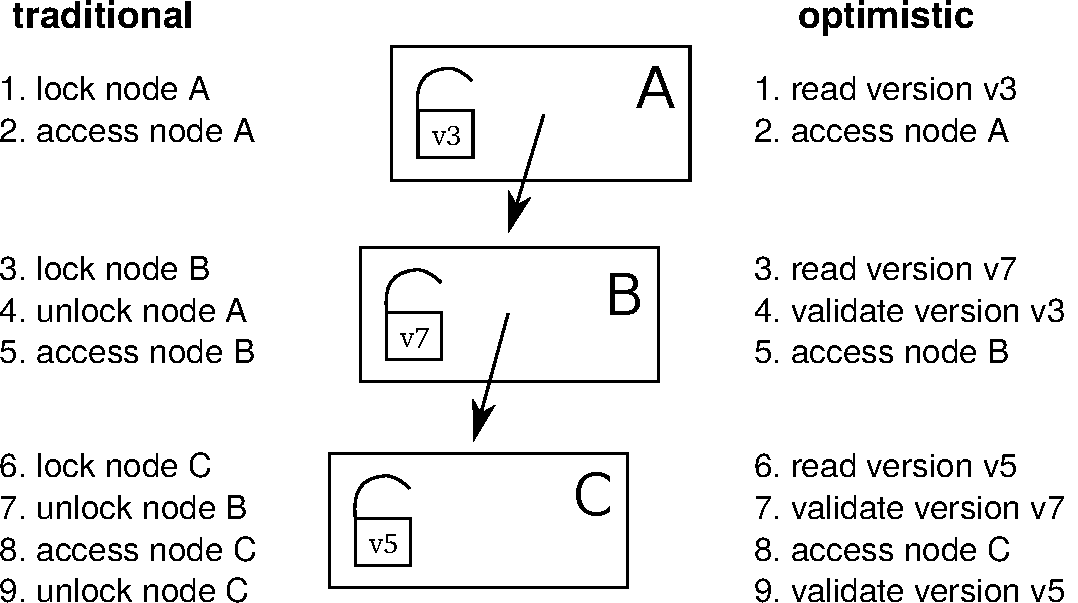
\includegraphics[width=0.65\linewidth]{olcall.pdf}
  \vspace{0.2cm}
  \caption{Comparison of a lookup operation in a 3-level tree using traditional lock coupling (left-hand side) vs.~optimistic lock coupling (right-hand side).}
  \label{fig:olc}
\end{figure}

The traditional and most common lock-based synchronization protocol for B-trees is lock coupling, which interleaves lock acquisitions while holding at most two locks at a time.
If, as we observed earlier, optimistic locks have similar semantics as traditional locks, it is natural to ask whether lock coupling can be combined with optimistic locks.
And indeed the answer is yes: One can almost mechanically translate traditional lock coupling code to optimistic lock coupling code.
This is illustrated in Figure~\ref{fig:olc}, which compares the traversal in a tree of height 3 using traditional and optimistic locks.
As the figure shows, the main difference is that locking is translated to reading the version and that unlocking becomes validation of the previously read version.
This simple change provides efficient lock-free tree traversal without the need to design a complex synchronization protocol.

It is important to emphasize the conceptual simplicity of OLC in comparison to data structures that use custom protocols like the Bw-tree~\cite{DBLP:conf/icde/LevandoskiLS13a}.
To implement lock-free access, the Bw-tree requires an indirection table, delta nodes, complex splitting and merging logic, retry logic, etc.
OLC, on the other hand, can directly be applied to B-trees mostly by adding the appropriate optimistic locking code and without modifying the node layout itself.
Therefore, OpenBw-Tree, an open source implementation of the Bw-tree, requires an order of magnitude more code than a B-tree based on OLC\footnote{Both implementations are available on GitHub: \url{https://github.com/wangziqi2016/index-microbench}}.
Given how difficult it is to develop, validate, and debug lock-free code, simplicity is obviously a major advantage.

\subsection{Correctness Aspects}

\begin{figure}
  % \centering
  %[basicstyle=\normalsize\ttfamily,showstringspaces=false,columns=fullflexible,breaklines=false,breakatwhitespace=true,numbers=none,numberstyle=\small,style=C,keepspaces=true]
\begin{lstlisting}[basicstyle=\ttfamily,language=C++,numbers=left,numberstyle=\small]
std::atomic<BTreeNode*> root;

// search for key in B+tree, returns payload in resultOut
bool lookup(Key key, Value& resultOut) {
   BTreeNode* node = root.load();
   uint64_t nodeVersion = node->readLockOrRestart();
   if (node != root.load()) // make sure the root is still the root
      restart();

   BTreeInner<Key>* parent = nullptr;
   uint64_t parentVersion = 0;

   while (node->isInner()) {
      auto inner = (BTreeInner*)node;

      // unlock parent and make current node the parent
      if (parent)
         parent->readUnlockOrRestart(parentVersion);
      parent = inner;
      parentVersion = nodeVersion;

      // search for next node
      node = inner->findChild(key);
      // validate 'inner' to ensure that 'node' pointer is valid
      inner->checkOrRestart(nodeVersion);
      // now it safe to dereference 'node' pointer (read its version)
      nodeVersion = node->readLockOrRestart();
   }

   // search in leaf and retrieve payload
   auto leaf = (BTreeLeaf*)node;
   bool success = leaf->findValue(key, resultOut);

   // unlock everything
   if (parent)
      parent->readUnlockOrRestart(parentVersion);
   node->readUnlockOrRestart(nodeVersion);

   return success;
}
\end{lstlisting}
  \vspace{0.2cm}
  \caption{B-tree lookup code using OLC. For simplicity, the restart logic is not shown.}
  \label{fig:lookup}
\end{figure}

So far, we have introduced the high-level ideas behind OLC and have stressed its similarity to traditional lock coupling.
Let us now discuss some cases where the close similarity between lock coupling and OLC breaks down.
To make this more concrete, we show the B-tree lookup code in Figure~\ref{fig:lookup}.
In the code, \texttt{readLockOrRestart} reads the lock version and \texttt{readUnlockOrRestart} validates that the read was correct.

One issue with OLC is that any pointer speculatively read from a node may point to invalid memory (if that node is modified concurrently).
Dereferencing such a pointer (e.g., to read its optimistic lock), may cause a segmentation fault or undefined behavior.
In the code shown in Figure~\ref{fig:lookup}, this problem is prevented by the extra check in line 25, which ensures that the read from the node containing the pointer was correct.
Without this additional validation, the code would in line 27 dereference the pointer speculatively read in line 23.
Note that the implementation of \texttt{checkOrRestart} is actually identical to \texttt{readUnlockOrRestart}.
We chose to give it a different name to highlight the fact that this extra check would not be necessary with read/write locks.

Another potential issue with optimistic locks is code that does not terminate.
Code that speculatively accesses a node, like an intra-node binary search, should be written in a way such that it always terminates---even in the presence of concurrent writes.
Otherwise, the validation code that detects the concurrent write will never run.
The binary search of a B-tree, for example, needs to be written in such a way that each comparison makes progress.
For some data structures that do not require loops in the traversal code (like ART) termination is trivially true.

\subsection{Implementation Details}

% implementation, efficiency
To implement an optimistic lock, one can combine the lock and the version counter into a single 64-bit\footnote{Even after subtracting one bit for the lock status, a back-of-the-envelope calculation can show that 63 bits are large enough to never overflow in practice.} word~\cite{artsync}.
A typical read operation will therefore merely consist of reading this version counter atomically.
In C++11 this can be implemented using the \texttt{std::atomic} type.

On x86, atomic reads are cheap because of x86's strong memory order guarantees.
No memory fences are required for sequentially-consistent loads, which are translated (by both GCC and clang) into standard \texttt{MOV} instructions.
Hence, the only effect of \texttt{std::atomic} for loads is preventing instruction re-ordering.
This makes version access and validation cheap.
Acquiring and releasing an optimistic lock in exclusive mode has comparable cost to a traditional lock:
A fairly expensive sequentially-consistent store is needed for acquiring a lock, while a standard \texttt{MOV} suffices for releasing it.
A simple sinlock-based implementation of optimistic locks can be found in the appendix of an earlier paper~\cite{artsync}.

OLC code must be able to handle restarts since validation or lock upgrade can fail due to concurrent writers.
Restarts can easily be implemented by wrapping the data structure operation in a loop (for simplicity not shown in Figure~\ref{fig:lookup}).
Such a loop also enables limiting the number of optimistic retry operations and falling back to pessimistic locking in cases of very heavy contention.
The ability to fall back to traditional locking is a major advantage of OLC in terms of robustness over lock-free approaches, which do not have this option.

In addition to the optimistic shared mode and the exclusive mode, optimistic locks also support a ``shared pessimistic'' mode, which physically acquires the lock in shared mode (allowing multiple concurrent readers but no writers).
This mode is useful for table (or range) scans that touch many tuples on a leaf page (which would otherwise easily abort).
Finally, let us mention that large range scans and table scans, should be broken up into several per-node traversals as is done in the LeanStore~\cite{leanstore} system.

Like all lock-free data structures, but unlike traditional locking and Hardware Transactional Memory~\cite{DBLP:conf/hpca/KarnagelDRLLSL14,DBLP:journals/pvldb/MakreshanskiLS15,htmtkde}, OLC requires care when deleting (and reusing) nodes.
The reason is that a deleting thread can never be sure that a node can be reclaimed because other threads might still be optimistically reading from that node.
Therefore, standard solutions like epoch-based reclamation~\cite{DBLP:conf/sosp/TuZKLM13}, hazard pointers~\cite{DBLP:journals/tpds/Michael04}, or optimized hazard pointers~\cite{DBLP:conf/spaa/BalmauGHZ16} need to be used.
These memory reclamation techniques are, however, largely orthogonal to the synchronization protocol itself.

%-lock-free is not a strong guarantee

\newpage
\section{Evaluation}\label{sec:evaluation}

Let us now experimentally evaluate the overhead and scalability of OLC.
For the experiments, we use an in-memory B+tree implemented in C++11 using templates, which is configured to use nodes of 4096 bytes, random 8 byte keys, and 8 byte payloads.
Based on this B-tree, we compare the following synchronization approaches:
\begin{itemize}
\item an OLC implementation\footnote{An almost identical OLC implementation is available on github: \url{https://github.com/wangziqi2016/index-microbench/tree/master/BTreeOLC}}
\item a variant based on traditional lock coupling and read/write locks
\item the unsynchronized B-tree, which obviously is only correct for read-only workloads but allows measuring the overhead of synchronization
\end{itemize}
Note that earlier work has compared the OLC implementation with a Bw-tree implementation~\cite{buzzword} and other state-of-the-art in-memory index structures.

We use a Haswell EP system with an Intel Xeon E5-2687W v3 CPU, which has 10 cores (20 ``Hyper-Threads'') and 25~MB of L3 cache.
The system is running Ubuntu 18.10 and we use GCC 8.2.0 to compile our code.
The CPU counters are obtained using the Linux perf API\footnote{We use the following convenience wrapper: \url{https://github.com/viktorleis/perfevent}}.

\begin{table}
  \caption{Performance and CPU counters for lookup and insert operations in a B-tree with 100M keys. We perform 100M operations and normalize the CPU counters by that number.}
  \label{tab:overhead}
  \centering
  \begin{tabular}{lrrrrrrr}\toprule
                    &         &        &        & instruc-  & L1     & L3     & branch \\
                    & threads & M op/s & cycles & tions & misses & misses & misses \\\midrule
lookup (no sync.)   & 1       & 1.72   & 2028   & 283     & 39.1   & 14.9   & 16.1   \\
lookup (OLC)        & 1       & 1.65   & 2107   & 370     & 43.9   & 15.1   & 16.7   \\
lookup (lock coup.) & 1       & 1.72   & 2078   & 365     & 42.3   & 16.9   & 15.7   \\\midrule
insert (no sync.)   & 1       & 1.51   & 2286   & 530     & 59.8   & 31.1   & 17.3   \\
insert (OLC)        & 1       & 1.50   & 2303   & 629     & 61.2   & 31.1   & 16.5   \\
insert (lock coup.) & 1       & 1.41   & 2473   & 644     & 61.0   & 31.0   & 17.2   \\\midrule
lookup (no sync.)   & 10      & 15.48  & 2058   & 283     & 38.6   & 15.5   & 16.0   \\
lookup (OLC)        & 10      & 14.60  & 2187   & 370     & 43.8   & 15.8   & 16.8   \\
lookup (lock coup.) & 10      & 5.71   & 5591   & 379     & 54.2   & 17.0   & 14.8   \\\midrule
insert (no sync.)   & 10      & -      & -      & -       & -      & -      & -      \\
insert (OLC)        & 10      & 10.46  & 2940   & 656     & 62.0   & 32.5   & 16.8   \\
insert (lock coup.) & 10      & 7.55   & 4161   & 667     & 75.0   & 28.6   & 16.2   \\
    \bottomrule
\end{tabular}
\end{table}

Table~\ref{tab:overhead} compares the performance and CPU counters for lookup and insert operations in a B-tree with 100M keys.
With {\em single-threaded} execution, we observe that all three approaches have very similar performance.
Adding traditional or optimistic locks to unsynchronized B-tree code results in up to 30\% of additional instructions without affecting single-threaded performance much.

\begin{figure}
  \centering
  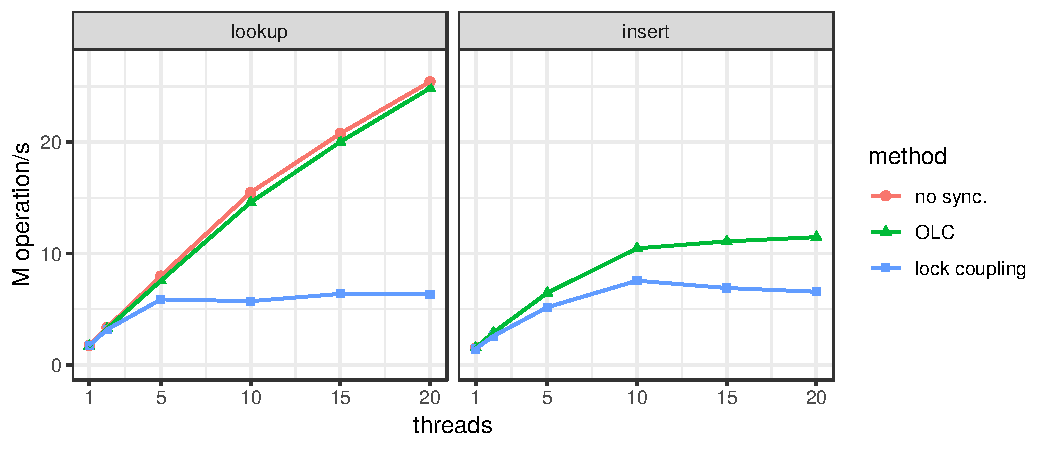
\includegraphics[width=\linewidth]{scale.pdf}
  \vspace{0.2cm}
  \caption{Scalability on 10-core system for B-tree operations (100M values).}
  \label{fig:scale}
\end{figure}

As Figure~\ref{fig:scale} shows, the results change dramatically once we use multiple threads.
For lookup, the scalability of OLC is near-linear up to 20 threads, even though the system has only 10 ``real cores''.
The OLC scalability for insert is also respectable (though not quite as linear because multi-threaded insertion approaches the memory bandwidth of our processor).
The figure also shows that the results of traditional lock coupling with read/write locks are significantly worse than OLC.
With 20 threads, lookup with OLC is 3.9$\times$ faster than traditional lock coupling.

\section{Summary}\label{sec:conc}

Optimistic Lock Coupling (OLC) is an effective synchronization method that combines the simplicity of traditional lock coupling with the superior scalability of lock-free approaches.
OLC is widely applicable and has already been successfully used to synchronize several data structures, including B-trees, binary search trees, and different trie variants.
These features make it highly attractive for modern database systems as well as performance-critical systems software in general.

\begin{thebibliography}{10}

\bibitem{DBLP:conf/spaa/BalmauGHZ16}
O.~Balmau, R.~Guerraoui, M.~Herlihy, and I.~Zablotchi.
\newblock Fast and robust memory reclamation for concurrent data structures.
\newblock In {\em SPAA}, 2016.

\bibitem{DBLP:journals/acta/BayerS77}
R.~Bayer and M.~Schkolnick.
\newblock Concurrency of operations on {B}-trees.
\newblock {\em Acta Informatica}, 9, 1977.

\bibitem{hot}
R.~Binna, E.~Zangerle, M.~Pichl, G.~Specht, and V.~Leis.
\newblock {HOT}: A height optimized trie index for main-memory database
  systems.
\newblock In {\em SIGMOD}, 2018.

\bibitem{DBLP:conf/ppopp/BronsonCCO10}
N.~G. Bronson, J.~Casper, H.~Chafi, and K.~Olukotun.
\newblock A practical concurrent binary search tree.
\newblock In {\em PPOPP}, 2010.

\bibitem{DBLP:conf/vldb/ChaHKK01}
S.~K. Cha, S.~Hwang, K.~Kim, and K.~Kwon.
\newblock Cache-conscious concurrency control of main-memory indexes on
  shared-memory multiprocessor systems.
\newblock In {\em VLDB}, 2001.

\bibitem{intel}
I.~Cutress.
\newblock {Intel} goes for 48-cores: {Cascade-AP} with multi-chip package
  coming soon.
\newblock
  \url{https://www.anandtech.com/show/13535/intel-goes-for-48cores-cascade-ap},
  2018 (accessed January, 2019).

\bibitem{DBLP:conf/cidr/FaleiroA17}
J.~M. Faleiro and D.~J. Abadi.
\newblock Latch-free synchronization in database systems: Silver bullet or
  fool's gold?
\newblock In {\em CIDR}, 2017.

\bibitem{DBLP:journals/ftdb/Graefe11}
G.~Graefe.
\newblock Modern {B}-tree techniques.
\newblock {\em Foundations and Trends in Databases}, 3(4), 2011.

\bibitem{DBLP:conf/hpca/KarnagelDRLLSL14}
T.~Karnagel, R.~Dementiev, R.~Rajwar, K.~Lai, T.~Legler, B.~Schlegel, and
  W.~Lehner.
\newblock Improving in-memory database index performance with
  {Intel}\({}^{\mbox{{\textregistered}}}\) transactional synchronization
  extensions.
\newblock In {\em HPCA}, 2014.

\bibitem{DBLP:journals/tods/LehmanY81}
P.~L. Lehman and S.~B. Yao.
\newblock Efficient locking for concurrent operations on {B}-trees.
\newblock {\em {ACM} Trans. Database Syst.}, 6(4), 1981.

\bibitem{leanstore}
V.~Leis, M.~Haubenschild, A.~Kemper, and T.~Neumann.
\newblock Leanstore: In-memory data management beyond main memory.
\newblock In {\em ICDE}, 2018.

\bibitem{art}
V.~Leis, A.~Kemper, and T.~Neumann.
\newblock The adaptive radix tree: {ARTful} indexing for main-memory databases.
\newblock In {\em ICDE}, 2013.

\bibitem{htmtkde}
V.~Leis, A.~Kemper, and T.~Neumann.
\newblock Scaling {HTM}-supported database transactions to many cores.
\newblock {\em {IEEE} Trans. Knowl. Data Eng.}, 28(2), 2016.

\bibitem{artsync}
V.~Leis, F.~Scheibner, A.~Kemper, and T.~Neumann.
\newblock The {ART} of practical synchronization.
\newblock In {\em DaMoN}, 2016.

\bibitem{DBLP:conf/icde/LevandoskiLS13a}
J.~J. Levandoski, D.~B. Lomet, and S.~Sengupta.
\newblock The {Bw}-tree: A {B}-tree for new hardware platforms.
\newblock In {\em ICDE}, 2013.

\bibitem{DBLP:journals/pvldb/MakreshanskiLS15}
D.~Makreshanski, J.~J. Levandoski, and R.~Stutsman.
\newblock To lock, swap, or elide: On the interplay of hardware transactional
  memory and lock-free indexing.
\newblock {\em {PVLDB}}, 8(11), 2015.

\bibitem{DBLP:dblp_conf/eurosys/MaoKM12}
Y.~Mao, E.~Kohler, and R.~T. Morris.
\newblock Cache craftiness for fast multicore key-value storage.
\newblock In {\em EuroSys}, 2012.

\bibitem{DBLP:journals/tpds/Michael04}
M.~M. Michael.
\newblock Hazard pointers: Safe memory reclamation for lock-free objects.
\newblock {\em {IEEE} Trans. Parallel Distrib. Syst.}, 15(6), 2004.

\bibitem{DBLP:journals/jacm/ShalevS06}
O.~Shalev and N.~Shavit.
\newblock Split-ordered lists: Lock-free extensible hash tables.
\newblock {\em J. {ACM}}, 53(3), 2006.

\bibitem{amd}
A.~Shilov.
\newblock {AMD} previews {EPYC} ‘{Rome}’ processor: Up to 64 {Zen} 2 cores.
\newblock
  \url{https://www.anandtech.com/show/13561/amd-previews-epyc-rome-processor-up-to-64-zen-2-cores},
  2018 (accessed January, 2019).

\bibitem{DBLP:conf/sosp/TuZKLM13}
S.~Tu, W.~Zheng, E.~Kohler, B.~Liskov, and S.~Madden.
\newblock Speedy transactions in multicore in-memory databases.
\newblock In {\em SOSP}, 2013.

\bibitem{buzzword}
Z.~Wang, A.~Pavlo, H.~Lim, V.~Leis, H.~Zhang, M.~Kaminsky, and D.~Andersen.
\newblock Building a {Bw}-tree takes more than just buzz words.
\newblock In {\em SIGMOD}, 2018.

\end{thebibliography}


%\bibliographystyle{abbrv}
%\bibliography{main}

\end{document}

\end{article}


\begin{article}
{Platform Design for Crowdsourcing and Future of Work}
{David Gross-Amblard, Atsuyuki Morishima, Saravanan Thirumuruganathan,Marion Tommasi, Ko Yoshida}
\graphicspath{{submissions/atsuyuki/}}
\pdfminorversion=5
\documentclass[11pt]{article}
\usepackage{deauthor,times,graphicx,caption,microtype}
\usepackage{hyperref}
\usepackage{listings}
\usepackage{booktabs}

\begin{document}

\title{Optimistic Lock Coupling: A Scalable and Efficient General-Purpose Synchronization Method}

\author{Viktor Leis, Michael Haubenschild\raisebox{0.9ex}{$\ast$}, Thomas Neumann\\ Technische Universit{\"a}t M{\"u}nchen \hspace{0.7cm} Tableau Software\raisebox{0.9ex}{$\ast$} \\ {\{leis,neumann\}{@}in.tum.de} \hspace{0.7cm} {mhaubenschild{@}tableau.com\raisebox{0.9ex}{$\ast$}}}

\maketitle

\begin{abstract}
As the number of cores on commodity processors continues to increase, scalability becomes more and more crucial for overall performance.
Scalable and efficient concurrent data structures are particularly important, as these are often the building blocks of parallel algorithms.
Unfortunately, traditional synchronization techniques based on fine-grained locking have been shown to be unscalable on modern multi-core CPUs.
Lock-free data structures, on the other hand, are extremely difficult to design and often incur significant overhead.

In this work, we make the case for Optimistic Lock Coupling as a practical alternative to both traditional locking and the lock-free approach.
We show that Optimistic Lock Coupling is highly scalable and almost as simple to implement as traditional lock coupling.
Another important advantage is that it is easily applicable to most tree-like data structures.
We therefore argue that Optimistic Lock Coupling, rather than a complex and error-prone custom synchronization protocol, should be the default choice for performance-critical data structures.
\end{abstract}

\section{Introduction}

% more and more cores
Today, Intel's commodity server processors have up to 28 cores and its upcoming microarchitecture will have up to 48 cores per socket~\cite{intel}.
Similarly, AMD currently stands at 32 cores and this number is expected to double in the next generation~\cite{amd}.
Since both platforms support simultaneous multithreading (also known as hyperthreading), affordable commodity servers (with up to two sockets) will soon routinely have between 100 and 200 hardware threads.

% data structure scalability is important
With such a high degree of hardware parallelism, efficient data processing crucially depends on how well concurrent data structures scale.
Internally, database systems use a plethora of data structures like table heaps, internal work queues, and, most importantly, index structures.
Any of these can easily become a scalability (and therefore overall performance) bottleneck on many-core CPUs.

% traditional synchronization: fine-grained locks, slow, cache invalidation
Traditionally, database systems synchronize internal data structures using fine-grained reader/writer locks\footnote{In this work, we focus on data structure synchronization rather than high-level transaction semantics and therefore use the term {\em lock} for what would typically be called {\em latch} in the database literature. We thus follow common computer science (rather than database) terminology.}.
Unfortunately, while fine-grained locking makes lock contention unlikely, it still results in bad scalability because lock acquisition and release require writing to shared memory.
Due to the way cache coherency is implemented on modern multi-core CPUs, these writes cause additional cache misses\footnote{The cache coherency protocol ensures that all copies of a cache line on other cores are invalidated before the write can proceed.} and the cache line containing the lock's internal data becomes a point of physical contention.
As a result, any frequently-accessed lock (e.g., the lock of the root node of a B-tree) severely limits scalability.

% lock-free bw-tree: no more latches, but indirections, extremely complex
Lock-free data structures like the Bw-tree~\cite{DBLP:conf/icde/LevandoskiLS13a} (a lock-free B-tree variant) or the Split-Ordered List~\cite{DBLP:journals/jacm/ShalevS06} (a lock-free hash table) do not acquire any locks and therefore generally scale much better than locking-based approaches (in particular for read-mostly workloads).
However, lock-free synchronization has other downsides:
First, it is very difficult and results in extremely complex and error-prone code (when compared to locking).
Second, because the functionality of atomic primitives provided by the hardware (e.g., atomically compare-and-swap 8 bytes) is limited, complex operations require additional indirections within the data structure.
For example, the Bw-tree requires an indirection table and the Split-Ordered List requires ``dummy nodes'', resulting in overhead due to additional cache misses.

% OLC for the win
In this paper we make the case for {\em Optimistic Lock Coupling (OLC)}, a synchronization method that combines some of the best properties of lock-based and lock-free synchronization.
OLC utilizes a special lock type that can be used in two modes:
The first mode is similar to a traditional mutex and excludes other threads by physically acquiring the underlying lock.
In the second mode, reads can proceed optimistically by validating a version counter that is embedded in the lock (similar to optimistic concurrency control).
The first mode is typically used by writers and the second mode by readers.
Besides this special lock type, OLC is based on the observation that optimistic lock validations can be interleaved/coupled---similar to the pair-wise interleaved lock acquisition of traditional lock coupling.
Hence, the name Optimistic Lock Coupling.

OLC has a number of desirable features:
\begin{itemize}
\item By reducing the number of writes to shared memory locations and thereby avoiding cache invalidations, it {\bf scales well} for most workloads.
\item In comparison to unsynchronized code, it requires few additional CPU instructions making it {\bf efficient}.
\item OLC is {\bf widely applicable} to different data structures. It has already been successfully used for synchronizing binary search trees~\cite{DBLP:conf/ppopp/BronsonCCO10}, tries~\cite{artsync}, trie/B-tree hybrids~\cite{DBLP:dblp_conf/eurosys/MaoKM12}, and B-trees~\cite{buzzword}.
\item In comparison to the lock-free paradigm, it is also {\bf easy to use} and requires few modifications to existing, single-threaded data structures.
\end{itemize}
Despite these positive features and its simplicity, OLC is not yet widely known.
The goal of this paper is therefore to popularize this simple idea and to make a case for it.
We argue that OLC deserves to be widely known.
It is a good default synchronization paradigm---more complex, data structure-specific protocols are seldom beneficial.

The rest of the paper is organized as follows.
Section~\ref{sec:related} discusses related work, tracing the history of OLC and its underlying ideas in the literature.
The core of the paper is Section~\ref{sec:olc}, which describes the ideas behind OLC and how it can be used to synchronize complex data structures.
In Section~\ref{sec:evaluation} we experimentally show that OLC has low overhead and scales well when used to synchronize an in-memory B-tree.
We summarize the paper in Section~\ref{sec:conc}.

\newpage
\section{Related Work}\label{sec:related}

Lock coupling has been proposed as a method for allowing concurrent operations on B-trees in 1977~\cite{DBLP:journals/acta/BayerS77}.
This traditional and still widely-used method, described in detail in Graefe's B-tree survey~\cite{DBLP:journals/ftdb/Graefe11}, is also called ``latch coupling'', ``hand-over-hand locking'', and ``crabbing''.
Because at most two locks are held at-a-time during tree traversal, this technique seemingly allows for a high degree of parallelism---in particular if read/write locks are used to enable inner nodes to be locked in shared mode.
However, as we show in Section~\ref{sec:evaluation}, on modern hardware lock acquisition (even in shared mode) results in suboptimal scalability.

An early alternative from 1981 is a B-tree variant called B-link tree~\cite{DBLP:journals/tods/LehmanY81}, which only holds a single lock at a time.
It is based on the observation that between the release of the parent lock and the acquisition of the child lock, the only ``dangerous'' thing that could have happened is the split of a child node (assuming one does not implement merge operations).
Thus, when a split happens, the key being searched might end up on a neighboring node to the right of the current child node.
A B-link tree traversal therefore detects this condition and, if needed, transparently proceeds to the neighboring node.
Releasing the parent lock early is highly beneficial when the child node needs to be fetched from disk.
For in-memory workloads, however, the B-link tree has the same scalability issues as lock coupling (it acquires just as many locks).

The next major advance, Optimistic Latch-Free Index Traversal (OLFIT)~\cite{DBLP:conf/vldb/ChaHKK01}, was proposed in 2001.
OLFIT introduced the idea of a combined lock/update counter, which we call {\em optimistic lock}. % , for lack of a better name,
Based on these per-node optimistic locks and the synchronization protocol of the B-link tree, OLFIT finally achieves good scalability on parallel processors.
The OLFIT protocol is fairly complex, as it requires both the non-trivial B-link protocol and optimistic locks.
Furthermore, like the B-link tree protocol, it does not support merging nodes, and is specific to B-trees (cannot easily be applied to other data structures).

In the following two decades, the growth of main-memory capacity led to much research into other data structures besides the venerable B-tree.
Particularly relevant for our discussion is Bronson et al.'s~\cite{DBLP:conf/ppopp/BronsonCCO10} concurrent binary search tree, which is based on optimistic version validation and has a sophisticated, data structure-specific synchronization protocol.
To the best of our knowledge, this 2010 paper is the first that, as part of its protocol, interleaves version validation across nodes---rather than validating each node separately like OLFIT.
In that paper, this idea is called ``hand-over-hand, optimistic validation'', while we prefer the term Optimistic Lock Coupling to highlight the close resemblance to traditional lock coupling.
Similarly, Mao et al.'s~\cite{DBLP:dblp_conf/eurosys/MaoKM12} Masstree (a concurrent hybrid trie/B-tree) is also based on the same ideas, but again uses them as part of a more complex protocol.

The Adaptive Radix Tree (ART)~\cite{art} is another recent in-memory data structure, which we proposed in 2013.
In contrast to the two data structures just mentioned, it was originally designed with single-threaded performance in mind without supporting concurrency.
To add support for concurrency, we initially started designing a custom protocol called Read-Optimized Write Exclusion (ROWEX)~\cite{artsync}, which turned out to be non-trivial and requires modifications of the underlying data structure\footnote{Note that ROWEX is already easier to apply to existing data structures than the lock-free approach. The difficulty depends on the data structure. Applying ROWEX is hard for B-trees with sorted keys and fairly easy for copy-on-write data structures like the Height Optimized Trie~\cite{hot}---with ART being somewhere in the middle.}.
However, fairly late in the project, we also realized, that OLC {\em alone} (rather than as part of a more complex protocol) is sufficient to synchronize ART.
No other changes to the data structure were necessary.
Both approaches were published and experimentally evaluated in a followup paper~\cite{artsync}, which shows that, despite its simplicity, OLC is efficient, scalable, and generally outperforms ROWEX.

Similar results were recently published regarding B-trees~\cite{buzzword}.
In this experimental study a simple OLC-based synchronization outperformed the Bw-tree~\cite{DBLP:conf/icde/LevandoskiLS13a}, a complex lock-free synchronization approach.
Another recent paper shows that for write-intensive workloads, locking often performs better than lock-free synchronization~\cite{DBLP:conf/cidr/FaleiroA17}.
These experiences indicate that OLC is a general-purpose synchronization paradigm and motivate the current paper.

%foster b-tree\cite{DBLP:journals/tods/GraefeKK12}
%Shasha theory~\cite{DBLP:journals/tods/ShashaG88}

\section{Optimistic Lock Coupling}\label{sec:olc}

% locks suck
The standard technique for inter-thread synchronization is mutual exclusion using fine-grained locks.
In a B-tree, for example, every node usually has its own associated lock, which is acquired before accessing that node.
The problem of locking on modern multi- and many-core processors is that lock acquisition and release require writing to the shared memory location that implements the lock.
This write causes exclusive ownership of the underlying cache line and invalidates copies of it on all other processor cores.
For hierarchical, tree-like data structures, the lock of the root node becomes a point of physical contention---even in read-only workloads and even when read/write locks are used.
Depending on the specific data structure, number of cores, cache coherency protocol implementation, cache topology, whether Non-Uniform Memory Access (NUMA) is used, locking can even result in multi-threaded performance that is worse than single-threaded execution.

% in b-trees this happens very much
The inherent pessimism of locking is particularly unfortunate for B-trees:
Despite the fact that logical modifications of the root node are very infrequent, every B-tree operation must lock the root node during tree traversal\footnote{To a lesser extent this obviously applies to all inner nodes, not just the root.}.
Even the vast majority of update operations (with the exception of splits and merges), only modify a single leaf node.
These observations indicate that a more optimistic approach, which does not require locking inner nodes, would be very beneficial for B-trees.

\subsection{Optimistic Locks}

% optimism to the rescue
As the name indicates, optimistic locks try to solve the scalability issues of traditional locks using an optimistic approach.
Instead of always physically acquiring locks, even for nodes that are unlikely to be modified simultaneously, after-the-fact validation is used to detect conflicts.
This is done by augmenting each lock with a version/update counter that is incremented on every modification.
Using this version counter, readers can optimistically proceed before validating that the version did not change to ensure that the read was safe.
If validation fails, the operation is restarted.

% details on opt locks
Using optimistic locks, a read-only node access (i.e., the majority of all operations in a B-tree) does not acquire the lock and does not increment the version counter.
Instead, it performs the following steps:
\begin{enumerate}
\item read lock version (restart if lock is not free)
\item access node
\item read the version again and validate that it has not changed in the meantime
\end{enumerate}
If the last step (the validation) fails, the operation has to be restarted.
Write operations, on the other hand, are more similar to traditional locking:
\begin{enumerate}
\item acquire lock (wait if necessary)
\item access/write to node
\item increment version and unlock node
\end{enumerate}
Writes can therefore protect a node from other writes.

% similar to locks
As we observed in an earlier paper~\cite{artsync}, because of similar semantics, optimistic locks can be hidden behind an API very similar to traditional read/write locks.
Both approaches have an exclusive lock mode, and acquiring a traditional lock in shared mode is analogous to optimistic version validation.
Furthermore, like with some implementations of traditional read/write locks, optimistic locks allow upgrading a shared lock to an exclusive lock.
Lock upgrades are, for example, used to avoid most B-tree update operations from having to lock inner nodes.
In our experience, the close resemblance of optimistic and traditional locks simplifies the reasoning about optimistic locks;
one can apply similar thinking as in traditional lock-based protocols.

\subsection{Lock Coupling with Optimistic Locks}

\begin{figure}
  \centering
  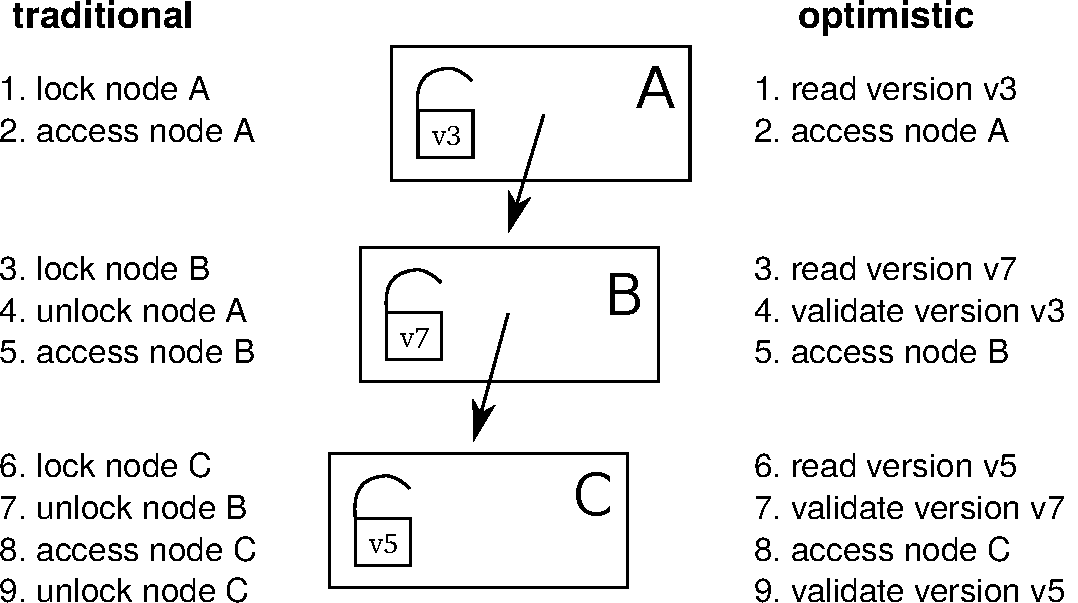
\includegraphics[width=0.65\linewidth]{olcall.pdf}
  \vspace{0.2cm}
  \caption{Comparison of a lookup operation in a 3-level tree using traditional lock coupling (left-hand side) vs.~optimistic lock coupling (right-hand side).}
  \label{fig:olc}
\end{figure}

The traditional and most common lock-based synchronization protocol for B-trees is lock coupling, which interleaves lock acquisitions while holding at most two locks at a time.
If, as we observed earlier, optimistic locks have similar semantics as traditional locks, it is natural to ask whether lock coupling can be combined with optimistic locks.
And indeed the answer is yes: One can almost mechanically translate traditional lock coupling code to optimistic lock coupling code.
This is illustrated in Figure~\ref{fig:olc}, which compares the traversal in a tree of height 3 using traditional and optimistic locks.
As the figure shows, the main difference is that locking is translated to reading the version and that unlocking becomes validation of the previously read version.
This simple change provides efficient lock-free tree traversal without the need to design a complex synchronization protocol.

It is important to emphasize the conceptual simplicity of OLC in comparison to data structures that use custom protocols like the Bw-tree~\cite{DBLP:conf/icde/LevandoskiLS13a}.
To implement lock-free access, the Bw-tree requires an indirection table, delta nodes, complex splitting and merging logic, retry logic, etc.
OLC, on the other hand, can directly be applied to B-trees mostly by adding the appropriate optimistic locking code and without modifying the node layout itself.
Therefore, OpenBw-Tree, an open source implementation of the Bw-tree, requires an order of magnitude more code than a B-tree based on OLC\footnote{Both implementations are available on GitHub: \url{https://github.com/wangziqi2016/index-microbench}}.
Given how difficult it is to develop, validate, and debug lock-free code, simplicity is obviously a major advantage.

\subsection{Correctness Aspects}

\begin{figure}
  % \centering
  %[basicstyle=\normalsize\ttfamily,showstringspaces=false,columns=fullflexible,breaklines=false,breakatwhitespace=true,numbers=none,numberstyle=\small,style=C,keepspaces=true]
\begin{lstlisting}[basicstyle=\ttfamily,language=C++,numbers=left,numberstyle=\small]
std::atomic<BTreeNode*> root;

// search for key in B+tree, returns payload in resultOut
bool lookup(Key key, Value& resultOut) {
   BTreeNode* node = root.load();
   uint64_t nodeVersion = node->readLockOrRestart();
   if (node != root.load()) // make sure the root is still the root
      restart();

   BTreeInner<Key>* parent = nullptr;
   uint64_t parentVersion = 0;

   while (node->isInner()) {
      auto inner = (BTreeInner*)node;

      // unlock parent and make current node the parent
      if (parent)
         parent->readUnlockOrRestart(parentVersion);
      parent = inner;
      parentVersion = nodeVersion;

      // search for next node
      node = inner->findChild(key);
      // validate 'inner' to ensure that 'node' pointer is valid
      inner->checkOrRestart(nodeVersion);
      // now it safe to dereference 'node' pointer (read its version)
      nodeVersion = node->readLockOrRestart();
   }

   // search in leaf and retrieve payload
   auto leaf = (BTreeLeaf*)node;
   bool success = leaf->findValue(key, resultOut);

   // unlock everything
   if (parent)
      parent->readUnlockOrRestart(parentVersion);
   node->readUnlockOrRestart(nodeVersion);

   return success;
}
\end{lstlisting}
  \vspace{0.2cm}
  \caption{B-tree lookup code using OLC. For simplicity, the restart logic is not shown.}
  \label{fig:lookup}
\end{figure}

So far, we have introduced the high-level ideas behind OLC and have stressed its similarity to traditional lock coupling.
Let us now discuss some cases where the close similarity between lock coupling and OLC breaks down.
To make this more concrete, we show the B-tree lookup code in Figure~\ref{fig:lookup}.
In the code, \texttt{readLockOrRestart} reads the lock version and \texttt{readUnlockOrRestart} validates that the read was correct.

One issue with OLC is that any pointer speculatively read from a node may point to invalid memory (if that node is modified concurrently).
Dereferencing such a pointer (e.g., to read its optimistic lock), may cause a segmentation fault or undefined behavior.
In the code shown in Figure~\ref{fig:lookup}, this problem is prevented by the extra check in line 25, which ensures that the read from the node containing the pointer was correct.
Without this additional validation, the code would in line 27 dereference the pointer speculatively read in line 23.
Note that the implementation of \texttt{checkOrRestart} is actually identical to \texttt{readUnlockOrRestart}.
We chose to give it a different name to highlight the fact that this extra check would not be necessary with read/write locks.

Another potential issue with optimistic locks is code that does not terminate.
Code that speculatively accesses a node, like an intra-node binary search, should be written in a way such that it always terminates---even in the presence of concurrent writes.
Otherwise, the validation code that detects the concurrent write will never run.
The binary search of a B-tree, for example, needs to be written in such a way that each comparison makes progress.
For some data structures that do not require loops in the traversal code (like ART) termination is trivially true.

\subsection{Implementation Details}

% implementation, efficiency
To implement an optimistic lock, one can combine the lock and the version counter into a single 64-bit\footnote{Even after subtracting one bit for the lock status, a back-of-the-envelope calculation can show that 63 bits are large enough to never overflow in practice.} word~\cite{artsync}.
A typical read operation will therefore merely consist of reading this version counter atomically.
In C++11 this can be implemented using the \texttt{std::atomic} type.

On x86, atomic reads are cheap because of x86's strong memory order guarantees.
No memory fences are required for sequentially-consistent loads, which are translated (by both GCC and clang) into standard \texttt{MOV} instructions.
Hence, the only effect of \texttt{std::atomic} for loads is preventing instruction re-ordering.
This makes version access and validation cheap.
Acquiring and releasing an optimistic lock in exclusive mode has comparable cost to a traditional lock:
A fairly expensive sequentially-consistent store is needed for acquiring a lock, while a standard \texttt{MOV} suffices for releasing it.
A simple sinlock-based implementation of optimistic locks can be found in the appendix of an earlier paper~\cite{artsync}.

OLC code must be able to handle restarts since validation or lock upgrade can fail due to concurrent writers.
Restarts can easily be implemented by wrapping the data structure operation in a loop (for simplicity not shown in Figure~\ref{fig:lookup}).
Such a loop also enables limiting the number of optimistic retry operations and falling back to pessimistic locking in cases of very heavy contention.
The ability to fall back to traditional locking is a major advantage of OLC in terms of robustness over lock-free approaches, which do not have this option.

In addition to the optimistic shared mode and the exclusive mode, optimistic locks also support a ``shared pessimistic'' mode, which physically acquires the lock in shared mode (allowing multiple concurrent readers but no writers).
This mode is useful for table (or range) scans that touch many tuples on a leaf page (which would otherwise easily abort).
Finally, let us mention that large range scans and table scans, should be broken up into several per-node traversals as is done in the LeanStore~\cite{leanstore} system.

Like all lock-free data structures, but unlike traditional locking and Hardware Transactional Memory~\cite{DBLP:conf/hpca/KarnagelDRLLSL14,DBLP:journals/pvldb/MakreshanskiLS15,htmtkde}, OLC requires care when deleting (and reusing) nodes.
The reason is that a deleting thread can never be sure that a node can be reclaimed because other threads might still be optimistically reading from that node.
Therefore, standard solutions like epoch-based reclamation~\cite{DBLP:conf/sosp/TuZKLM13}, hazard pointers~\cite{DBLP:journals/tpds/Michael04}, or optimized hazard pointers~\cite{DBLP:conf/spaa/BalmauGHZ16} need to be used.
These memory reclamation techniques are, however, largely orthogonal to the synchronization protocol itself.

%-lock-free is not a strong guarantee

\newpage
\section{Evaluation}\label{sec:evaluation}

Let us now experimentally evaluate the overhead and scalability of OLC.
For the experiments, we use an in-memory B+tree implemented in C++11 using templates, which is configured to use nodes of 4096 bytes, random 8 byte keys, and 8 byte payloads.
Based on this B-tree, we compare the following synchronization approaches:
\begin{itemize}
\item an OLC implementation\footnote{An almost identical OLC implementation is available on github: \url{https://github.com/wangziqi2016/index-microbench/tree/master/BTreeOLC}}
\item a variant based on traditional lock coupling and read/write locks
\item the unsynchronized B-tree, which obviously is only correct for read-only workloads but allows measuring the overhead of synchronization
\end{itemize}
Note that earlier work has compared the OLC implementation with a Bw-tree implementation~\cite{buzzword} and other state-of-the-art in-memory index structures.

We use a Haswell EP system with an Intel Xeon E5-2687W v3 CPU, which has 10 cores (20 ``Hyper-Threads'') and 25~MB of L3 cache.
The system is running Ubuntu 18.10 and we use GCC 8.2.0 to compile our code.
The CPU counters are obtained using the Linux perf API\footnote{We use the following convenience wrapper: \url{https://github.com/viktorleis/perfevent}}.

\begin{table}
  \caption{Performance and CPU counters for lookup and insert operations in a B-tree with 100M keys. We perform 100M operations and normalize the CPU counters by that number.}
  \label{tab:overhead}
  \centering
  \begin{tabular}{lrrrrrrr}\toprule
                    &         &        &        & instruc-  & L1     & L3     & branch \\
                    & threads & M op/s & cycles & tions & misses & misses & misses \\\midrule
lookup (no sync.)   & 1       & 1.72   & 2028   & 283     & 39.1   & 14.9   & 16.1   \\
lookup (OLC)        & 1       & 1.65   & 2107   & 370     & 43.9   & 15.1   & 16.7   \\
lookup (lock coup.) & 1       & 1.72   & 2078   & 365     & 42.3   & 16.9   & 15.7   \\\midrule
insert (no sync.)   & 1       & 1.51   & 2286   & 530     & 59.8   & 31.1   & 17.3   \\
insert (OLC)        & 1       & 1.50   & 2303   & 629     & 61.2   & 31.1   & 16.5   \\
insert (lock coup.) & 1       & 1.41   & 2473   & 644     & 61.0   & 31.0   & 17.2   \\\midrule
lookup (no sync.)   & 10      & 15.48  & 2058   & 283     & 38.6   & 15.5   & 16.0   \\
lookup (OLC)        & 10      & 14.60  & 2187   & 370     & 43.8   & 15.8   & 16.8   \\
lookup (lock coup.) & 10      & 5.71   & 5591   & 379     & 54.2   & 17.0   & 14.8   \\\midrule
insert (no sync.)   & 10      & -      & -      & -       & -      & -      & -      \\
insert (OLC)        & 10      & 10.46  & 2940   & 656     & 62.0   & 32.5   & 16.8   \\
insert (lock coup.) & 10      & 7.55   & 4161   & 667     & 75.0   & 28.6   & 16.2   \\
    \bottomrule
\end{tabular}
\end{table}

Table~\ref{tab:overhead} compares the performance and CPU counters for lookup and insert operations in a B-tree with 100M keys.
With {\em single-threaded} execution, we observe that all three approaches have very similar performance.
Adding traditional or optimistic locks to unsynchronized B-tree code results in up to 30\% of additional instructions without affecting single-threaded performance much.

\begin{figure}
  \centering
  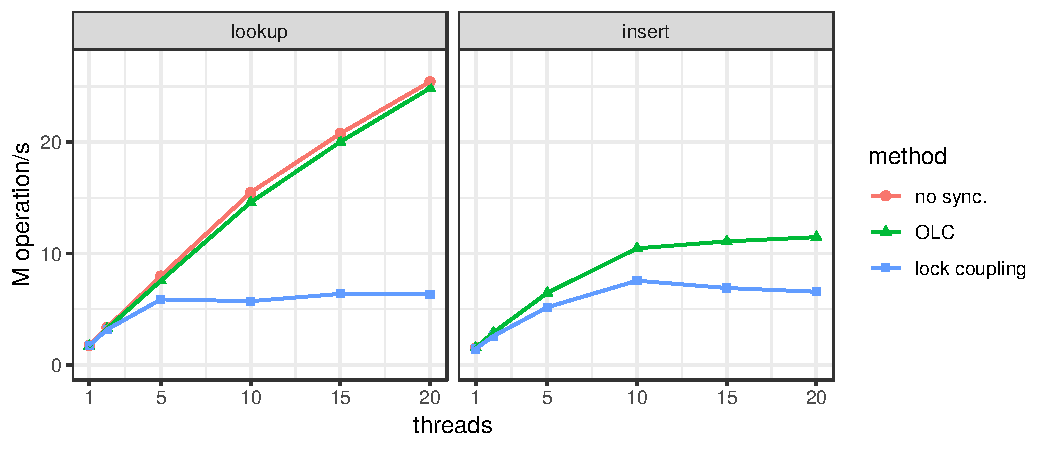
\includegraphics[width=\linewidth]{scale.pdf}
  \vspace{0.2cm}
  \caption{Scalability on 10-core system for B-tree operations (100M values).}
  \label{fig:scale}
\end{figure}

As Figure~\ref{fig:scale} shows, the results change dramatically once we use multiple threads.
For lookup, the scalability of OLC is near-linear up to 20 threads, even though the system has only 10 ``real cores''.
The OLC scalability for insert is also respectable (though not quite as linear because multi-threaded insertion approaches the memory bandwidth of our processor).
The figure also shows that the results of traditional lock coupling with read/write locks are significantly worse than OLC.
With 20 threads, lookup with OLC is 3.9$\times$ faster than traditional lock coupling.

\section{Summary}\label{sec:conc}

Optimistic Lock Coupling (OLC) is an effective synchronization method that combines the simplicity of traditional lock coupling with the superior scalability of lock-free approaches.
OLC is widely applicable and has already been successfully used to synchronize several data structures, including B-trees, binary search trees, and different trie variants.
These features make it highly attractive for modern database systems as well as performance-critical systems software in general.

\begin{thebibliography}{10}

\bibitem{DBLP:conf/spaa/BalmauGHZ16}
O.~Balmau, R.~Guerraoui, M.~Herlihy, and I.~Zablotchi.
\newblock Fast and robust memory reclamation for concurrent data structures.
\newblock In {\em SPAA}, 2016.

\bibitem{DBLP:journals/acta/BayerS77}
R.~Bayer and M.~Schkolnick.
\newblock Concurrency of operations on {B}-trees.
\newblock {\em Acta Informatica}, 9, 1977.

\bibitem{hot}
R.~Binna, E.~Zangerle, M.~Pichl, G.~Specht, and V.~Leis.
\newblock {HOT}: A height optimized trie index for main-memory database
  systems.
\newblock In {\em SIGMOD}, 2018.

\bibitem{DBLP:conf/ppopp/BronsonCCO10}
N.~G. Bronson, J.~Casper, H.~Chafi, and K.~Olukotun.
\newblock A practical concurrent binary search tree.
\newblock In {\em PPOPP}, 2010.

\bibitem{DBLP:conf/vldb/ChaHKK01}
S.~K. Cha, S.~Hwang, K.~Kim, and K.~Kwon.
\newblock Cache-conscious concurrency control of main-memory indexes on
  shared-memory multiprocessor systems.
\newblock In {\em VLDB}, 2001.

\bibitem{intel}
I.~Cutress.
\newblock {Intel} goes for 48-cores: {Cascade-AP} with multi-chip package
  coming soon.
\newblock
  \url{https://www.anandtech.com/show/13535/intel-goes-for-48cores-cascade-ap},
  2018 (accessed January, 2019).

\bibitem{DBLP:conf/cidr/FaleiroA17}
J.~M. Faleiro and D.~J. Abadi.
\newblock Latch-free synchronization in database systems: Silver bullet or
  fool's gold?
\newblock In {\em CIDR}, 2017.

\bibitem{DBLP:journals/ftdb/Graefe11}
G.~Graefe.
\newblock Modern {B}-tree techniques.
\newblock {\em Foundations and Trends in Databases}, 3(4), 2011.

\bibitem{DBLP:conf/hpca/KarnagelDRLLSL14}
T.~Karnagel, R.~Dementiev, R.~Rajwar, K.~Lai, T.~Legler, B.~Schlegel, and
  W.~Lehner.
\newblock Improving in-memory database index performance with
  {Intel}\({}^{\mbox{{\textregistered}}}\) transactional synchronization
  extensions.
\newblock In {\em HPCA}, 2014.

\bibitem{DBLP:journals/tods/LehmanY81}
P.~L. Lehman and S.~B. Yao.
\newblock Efficient locking for concurrent operations on {B}-trees.
\newblock {\em {ACM} Trans. Database Syst.}, 6(4), 1981.

\bibitem{leanstore}
V.~Leis, M.~Haubenschild, A.~Kemper, and T.~Neumann.
\newblock Leanstore: In-memory data management beyond main memory.
\newblock In {\em ICDE}, 2018.

\bibitem{art}
V.~Leis, A.~Kemper, and T.~Neumann.
\newblock The adaptive radix tree: {ARTful} indexing for main-memory databases.
\newblock In {\em ICDE}, 2013.

\bibitem{htmtkde}
V.~Leis, A.~Kemper, and T.~Neumann.
\newblock Scaling {HTM}-supported database transactions to many cores.
\newblock {\em {IEEE} Trans. Knowl. Data Eng.}, 28(2), 2016.

\bibitem{artsync}
V.~Leis, F.~Scheibner, A.~Kemper, and T.~Neumann.
\newblock The {ART} of practical synchronization.
\newblock In {\em DaMoN}, 2016.

\bibitem{DBLP:conf/icde/LevandoskiLS13a}
J.~J. Levandoski, D.~B. Lomet, and S.~Sengupta.
\newblock The {Bw}-tree: A {B}-tree for new hardware platforms.
\newblock In {\em ICDE}, 2013.

\bibitem{DBLP:journals/pvldb/MakreshanskiLS15}
D.~Makreshanski, J.~J. Levandoski, and R.~Stutsman.
\newblock To lock, swap, or elide: On the interplay of hardware transactional
  memory and lock-free indexing.
\newblock {\em {PVLDB}}, 8(11), 2015.

\bibitem{DBLP:dblp_conf/eurosys/MaoKM12}
Y.~Mao, E.~Kohler, and R.~T. Morris.
\newblock Cache craftiness for fast multicore key-value storage.
\newblock In {\em EuroSys}, 2012.

\bibitem{DBLP:journals/tpds/Michael04}
M.~M. Michael.
\newblock Hazard pointers: Safe memory reclamation for lock-free objects.
\newblock {\em {IEEE} Trans. Parallel Distrib. Syst.}, 15(6), 2004.

\bibitem{DBLP:journals/jacm/ShalevS06}
O.~Shalev and N.~Shavit.
\newblock Split-ordered lists: Lock-free extensible hash tables.
\newblock {\em J. {ACM}}, 53(3), 2006.

\bibitem{amd}
A.~Shilov.
\newblock {AMD} previews {EPYC} ‘{Rome}’ processor: Up to 64 {Zen} 2 cores.
\newblock
  \url{https://www.anandtech.com/show/13561/amd-previews-epyc-rome-processor-up-to-64-zen-2-cores},
  2018 (accessed January, 2019).

\bibitem{DBLP:conf/sosp/TuZKLM13}
S.~Tu, W.~Zheng, E.~Kohler, B.~Liskov, and S.~Madden.
\newblock Speedy transactions in multicore in-memory databases.
\newblock In {\em SOSP}, 2013.

\bibitem{buzzword}
Z.~Wang, A.~Pavlo, H.~Lim, V.~Leis, H.~Zhang, M.~Kaminsky, and D.~Andersen.
\newblock Building a {Bw}-tree takes more than just buzz words.
\newblock In {\em SIGMOD}, 2018.

\end{thebibliography}


%\bibliographystyle{abbrv}
%\bibliography{main}

\end{document}

\end{article}



\begin{article}
{On Benchmarking for Crowdsourcing and Future of Work Platforms}
{Ria Mae Borromeo, Lei Chen, Abhishek Dubey, Sudeepa Roy, Saravanan Thirumuruganathan}
\graphicspath{{submissions/Learning/}}
\pdfminorversion=5
\documentclass[11pt]{article}
\usepackage{deauthor,times,graphicx,caption,microtype}
\usepackage{hyperref}
\usepackage{listings}
\usepackage{booktabs}

\begin{document}

\title{Optimistic Lock Coupling: A Scalable and Efficient General-Purpose Synchronization Method}

\author{Viktor Leis, Michael Haubenschild\raisebox{0.9ex}{$\ast$}, Thomas Neumann\\ Technische Universit{\"a}t M{\"u}nchen \hspace{0.7cm} Tableau Software\raisebox{0.9ex}{$\ast$} \\ {\{leis,neumann\}{@}in.tum.de} \hspace{0.7cm} {mhaubenschild{@}tableau.com\raisebox{0.9ex}{$\ast$}}}

\maketitle

\begin{abstract}
As the number of cores on commodity processors continues to increase, scalability becomes more and more crucial for overall performance.
Scalable and efficient concurrent data structures are particularly important, as these are often the building blocks of parallel algorithms.
Unfortunately, traditional synchronization techniques based on fine-grained locking have been shown to be unscalable on modern multi-core CPUs.
Lock-free data structures, on the other hand, are extremely difficult to design and often incur significant overhead.

In this work, we make the case for Optimistic Lock Coupling as a practical alternative to both traditional locking and the lock-free approach.
We show that Optimistic Lock Coupling is highly scalable and almost as simple to implement as traditional lock coupling.
Another important advantage is that it is easily applicable to most tree-like data structures.
We therefore argue that Optimistic Lock Coupling, rather than a complex and error-prone custom synchronization protocol, should be the default choice for performance-critical data structures.
\end{abstract}

\section{Introduction}

% more and more cores
Today, Intel's commodity server processors have up to 28 cores and its upcoming microarchitecture will have up to 48 cores per socket~\cite{intel}.
Similarly, AMD currently stands at 32 cores and this number is expected to double in the next generation~\cite{amd}.
Since both platforms support simultaneous multithreading (also known as hyperthreading), affordable commodity servers (with up to two sockets) will soon routinely have between 100 and 200 hardware threads.

% data structure scalability is important
With such a high degree of hardware parallelism, efficient data processing crucially depends on how well concurrent data structures scale.
Internally, database systems use a plethora of data structures like table heaps, internal work queues, and, most importantly, index structures.
Any of these can easily become a scalability (and therefore overall performance) bottleneck on many-core CPUs.

% traditional synchronization: fine-grained locks, slow, cache invalidation
Traditionally, database systems synchronize internal data structures using fine-grained reader/writer locks\footnote{In this work, we focus on data structure synchronization rather than high-level transaction semantics and therefore use the term {\em lock} for what would typically be called {\em latch} in the database literature. We thus follow common computer science (rather than database) terminology.}.
Unfortunately, while fine-grained locking makes lock contention unlikely, it still results in bad scalability because lock acquisition and release require writing to shared memory.
Due to the way cache coherency is implemented on modern multi-core CPUs, these writes cause additional cache misses\footnote{The cache coherency protocol ensures that all copies of a cache line on other cores are invalidated before the write can proceed.} and the cache line containing the lock's internal data becomes a point of physical contention.
As a result, any frequently-accessed lock (e.g., the lock of the root node of a B-tree) severely limits scalability.

% lock-free bw-tree: no more latches, but indirections, extremely complex
Lock-free data structures like the Bw-tree~\cite{DBLP:conf/icde/LevandoskiLS13a} (a lock-free B-tree variant) or the Split-Ordered List~\cite{DBLP:journals/jacm/ShalevS06} (a lock-free hash table) do not acquire any locks and therefore generally scale much better than locking-based approaches (in particular for read-mostly workloads).
However, lock-free synchronization has other downsides:
First, it is very difficult and results in extremely complex and error-prone code (when compared to locking).
Second, because the functionality of atomic primitives provided by the hardware (e.g., atomically compare-and-swap 8 bytes) is limited, complex operations require additional indirections within the data structure.
For example, the Bw-tree requires an indirection table and the Split-Ordered List requires ``dummy nodes'', resulting in overhead due to additional cache misses.

% OLC for the win
In this paper we make the case for {\em Optimistic Lock Coupling (OLC)}, a synchronization method that combines some of the best properties of lock-based and lock-free synchronization.
OLC utilizes a special lock type that can be used in two modes:
The first mode is similar to a traditional mutex and excludes other threads by physically acquiring the underlying lock.
In the second mode, reads can proceed optimistically by validating a version counter that is embedded in the lock (similar to optimistic concurrency control).
The first mode is typically used by writers and the second mode by readers.
Besides this special lock type, OLC is based on the observation that optimistic lock validations can be interleaved/coupled---similar to the pair-wise interleaved lock acquisition of traditional lock coupling.
Hence, the name Optimistic Lock Coupling.

OLC has a number of desirable features:
\begin{itemize}
\item By reducing the number of writes to shared memory locations and thereby avoiding cache invalidations, it {\bf scales well} for most workloads.
\item In comparison to unsynchronized code, it requires few additional CPU instructions making it {\bf efficient}.
\item OLC is {\bf widely applicable} to different data structures. It has already been successfully used for synchronizing binary search trees~\cite{DBLP:conf/ppopp/BronsonCCO10}, tries~\cite{artsync}, trie/B-tree hybrids~\cite{DBLP:dblp_conf/eurosys/MaoKM12}, and B-trees~\cite{buzzword}.
\item In comparison to the lock-free paradigm, it is also {\bf easy to use} and requires few modifications to existing, single-threaded data structures.
\end{itemize}
Despite these positive features and its simplicity, OLC is not yet widely known.
The goal of this paper is therefore to popularize this simple idea and to make a case for it.
We argue that OLC deserves to be widely known.
It is a good default synchronization paradigm---more complex, data structure-specific protocols are seldom beneficial.

The rest of the paper is organized as follows.
Section~\ref{sec:related} discusses related work, tracing the history of OLC and its underlying ideas in the literature.
The core of the paper is Section~\ref{sec:olc}, which describes the ideas behind OLC and how it can be used to synchronize complex data structures.
In Section~\ref{sec:evaluation} we experimentally show that OLC has low overhead and scales well when used to synchronize an in-memory B-tree.
We summarize the paper in Section~\ref{sec:conc}.

\newpage
\section{Related Work}\label{sec:related}

Lock coupling has been proposed as a method for allowing concurrent operations on B-trees in 1977~\cite{DBLP:journals/acta/BayerS77}.
This traditional and still widely-used method, described in detail in Graefe's B-tree survey~\cite{DBLP:journals/ftdb/Graefe11}, is also called ``latch coupling'', ``hand-over-hand locking'', and ``crabbing''.
Because at most two locks are held at-a-time during tree traversal, this technique seemingly allows for a high degree of parallelism---in particular if read/write locks are used to enable inner nodes to be locked in shared mode.
However, as we show in Section~\ref{sec:evaluation}, on modern hardware lock acquisition (even in shared mode) results in suboptimal scalability.

An early alternative from 1981 is a B-tree variant called B-link tree~\cite{DBLP:journals/tods/LehmanY81}, which only holds a single lock at a time.
It is based on the observation that between the release of the parent lock and the acquisition of the child lock, the only ``dangerous'' thing that could have happened is the split of a child node (assuming one does not implement merge operations).
Thus, when a split happens, the key being searched might end up on a neighboring node to the right of the current child node.
A B-link tree traversal therefore detects this condition and, if needed, transparently proceeds to the neighboring node.
Releasing the parent lock early is highly beneficial when the child node needs to be fetched from disk.
For in-memory workloads, however, the B-link tree has the same scalability issues as lock coupling (it acquires just as many locks).

The next major advance, Optimistic Latch-Free Index Traversal (OLFIT)~\cite{DBLP:conf/vldb/ChaHKK01}, was proposed in 2001.
OLFIT introduced the idea of a combined lock/update counter, which we call {\em optimistic lock}. % , for lack of a better name,
Based on these per-node optimistic locks and the synchronization protocol of the B-link tree, OLFIT finally achieves good scalability on parallel processors.
The OLFIT protocol is fairly complex, as it requires both the non-trivial B-link protocol and optimistic locks.
Furthermore, like the B-link tree protocol, it does not support merging nodes, and is specific to B-trees (cannot easily be applied to other data structures).

In the following two decades, the growth of main-memory capacity led to much research into other data structures besides the venerable B-tree.
Particularly relevant for our discussion is Bronson et al.'s~\cite{DBLP:conf/ppopp/BronsonCCO10} concurrent binary search tree, which is based on optimistic version validation and has a sophisticated, data structure-specific synchronization protocol.
To the best of our knowledge, this 2010 paper is the first that, as part of its protocol, interleaves version validation across nodes---rather than validating each node separately like OLFIT.
In that paper, this idea is called ``hand-over-hand, optimistic validation'', while we prefer the term Optimistic Lock Coupling to highlight the close resemblance to traditional lock coupling.
Similarly, Mao et al.'s~\cite{DBLP:dblp_conf/eurosys/MaoKM12} Masstree (a concurrent hybrid trie/B-tree) is also based on the same ideas, but again uses them as part of a more complex protocol.

The Adaptive Radix Tree (ART)~\cite{art} is another recent in-memory data structure, which we proposed in 2013.
In contrast to the two data structures just mentioned, it was originally designed with single-threaded performance in mind without supporting concurrency.
To add support for concurrency, we initially started designing a custom protocol called Read-Optimized Write Exclusion (ROWEX)~\cite{artsync}, which turned out to be non-trivial and requires modifications of the underlying data structure\footnote{Note that ROWEX is already easier to apply to existing data structures than the lock-free approach. The difficulty depends on the data structure. Applying ROWEX is hard for B-trees with sorted keys and fairly easy for copy-on-write data structures like the Height Optimized Trie~\cite{hot}---with ART being somewhere in the middle.}.
However, fairly late in the project, we also realized, that OLC {\em alone} (rather than as part of a more complex protocol) is sufficient to synchronize ART.
No other changes to the data structure were necessary.
Both approaches were published and experimentally evaluated in a followup paper~\cite{artsync}, which shows that, despite its simplicity, OLC is efficient, scalable, and generally outperforms ROWEX.

Similar results were recently published regarding B-trees~\cite{buzzword}.
In this experimental study a simple OLC-based synchronization outperformed the Bw-tree~\cite{DBLP:conf/icde/LevandoskiLS13a}, a complex lock-free synchronization approach.
Another recent paper shows that for write-intensive workloads, locking often performs better than lock-free synchronization~\cite{DBLP:conf/cidr/FaleiroA17}.
These experiences indicate that OLC is a general-purpose synchronization paradigm and motivate the current paper.

%foster b-tree\cite{DBLP:journals/tods/GraefeKK12}
%Shasha theory~\cite{DBLP:journals/tods/ShashaG88}

\section{Optimistic Lock Coupling}\label{sec:olc}

% locks suck
The standard technique for inter-thread synchronization is mutual exclusion using fine-grained locks.
In a B-tree, for example, every node usually has its own associated lock, which is acquired before accessing that node.
The problem of locking on modern multi- and many-core processors is that lock acquisition and release require writing to the shared memory location that implements the lock.
This write causes exclusive ownership of the underlying cache line and invalidates copies of it on all other processor cores.
For hierarchical, tree-like data structures, the lock of the root node becomes a point of physical contention---even in read-only workloads and even when read/write locks are used.
Depending on the specific data structure, number of cores, cache coherency protocol implementation, cache topology, whether Non-Uniform Memory Access (NUMA) is used, locking can even result in multi-threaded performance that is worse than single-threaded execution.

% in b-trees this happens very much
The inherent pessimism of locking is particularly unfortunate for B-trees:
Despite the fact that logical modifications of the root node are very infrequent, every B-tree operation must lock the root node during tree traversal\footnote{To a lesser extent this obviously applies to all inner nodes, not just the root.}.
Even the vast majority of update operations (with the exception of splits and merges), only modify a single leaf node.
These observations indicate that a more optimistic approach, which does not require locking inner nodes, would be very beneficial for B-trees.

\subsection{Optimistic Locks}

% optimism to the rescue
As the name indicates, optimistic locks try to solve the scalability issues of traditional locks using an optimistic approach.
Instead of always physically acquiring locks, even for nodes that are unlikely to be modified simultaneously, after-the-fact validation is used to detect conflicts.
This is done by augmenting each lock with a version/update counter that is incremented on every modification.
Using this version counter, readers can optimistically proceed before validating that the version did not change to ensure that the read was safe.
If validation fails, the operation is restarted.

% details on opt locks
Using optimistic locks, a read-only node access (i.e., the majority of all operations in a B-tree) does not acquire the lock and does not increment the version counter.
Instead, it performs the following steps:
\begin{enumerate}
\item read lock version (restart if lock is not free)
\item access node
\item read the version again and validate that it has not changed in the meantime
\end{enumerate}
If the last step (the validation) fails, the operation has to be restarted.
Write operations, on the other hand, are more similar to traditional locking:
\begin{enumerate}
\item acquire lock (wait if necessary)
\item access/write to node
\item increment version and unlock node
\end{enumerate}
Writes can therefore protect a node from other writes.

% similar to locks
As we observed in an earlier paper~\cite{artsync}, because of similar semantics, optimistic locks can be hidden behind an API very similar to traditional read/write locks.
Both approaches have an exclusive lock mode, and acquiring a traditional lock in shared mode is analogous to optimistic version validation.
Furthermore, like with some implementations of traditional read/write locks, optimistic locks allow upgrading a shared lock to an exclusive lock.
Lock upgrades are, for example, used to avoid most B-tree update operations from having to lock inner nodes.
In our experience, the close resemblance of optimistic and traditional locks simplifies the reasoning about optimistic locks;
one can apply similar thinking as in traditional lock-based protocols.

\subsection{Lock Coupling with Optimistic Locks}

\begin{figure}
  \centering
  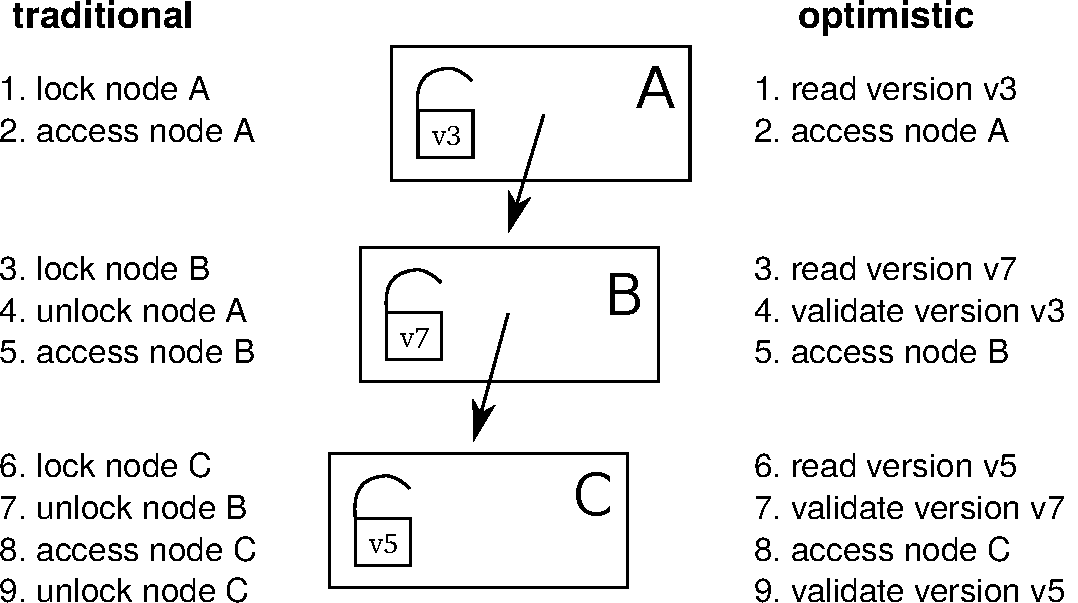
\includegraphics[width=0.65\linewidth]{olcall.pdf}
  \vspace{0.2cm}
  \caption{Comparison of a lookup operation in a 3-level tree using traditional lock coupling (left-hand side) vs.~optimistic lock coupling (right-hand side).}
  \label{fig:olc}
\end{figure}

The traditional and most common lock-based synchronization protocol for B-trees is lock coupling, which interleaves lock acquisitions while holding at most two locks at a time.
If, as we observed earlier, optimistic locks have similar semantics as traditional locks, it is natural to ask whether lock coupling can be combined with optimistic locks.
And indeed the answer is yes: One can almost mechanically translate traditional lock coupling code to optimistic lock coupling code.
This is illustrated in Figure~\ref{fig:olc}, which compares the traversal in a tree of height 3 using traditional and optimistic locks.
As the figure shows, the main difference is that locking is translated to reading the version and that unlocking becomes validation of the previously read version.
This simple change provides efficient lock-free tree traversal without the need to design a complex synchronization protocol.

It is important to emphasize the conceptual simplicity of OLC in comparison to data structures that use custom protocols like the Bw-tree~\cite{DBLP:conf/icde/LevandoskiLS13a}.
To implement lock-free access, the Bw-tree requires an indirection table, delta nodes, complex splitting and merging logic, retry logic, etc.
OLC, on the other hand, can directly be applied to B-trees mostly by adding the appropriate optimistic locking code and without modifying the node layout itself.
Therefore, OpenBw-Tree, an open source implementation of the Bw-tree, requires an order of magnitude more code than a B-tree based on OLC\footnote{Both implementations are available on GitHub: \url{https://github.com/wangziqi2016/index-microbench}}.
Given how difficult it is to develop, validate, and debug lock-free code, simplicity is obviously a major advantage.

\subsection{Correctness Aspects}

\begin{figure}
  % \centering
  %[basicstyle=\normalsize\ttfamily,showstringspaces=false,columns=fullflexible,breaklines=false,breakatwhitespace=true,numbers=none,numberstyle=\small,style=C,keepspaces=true]
\begin{lstlisting}[basicstyle=\ttfamily,language=C++,numbers=left,numberstyle=\small]
std::atomic<BTreeNode*> root;

// search for key in B+tree, returns payload in resultOut
bool lookup(Key key, Value& resultOut) {
   BTreeNode* node = root.load();
   uint64_t nodeVersion = node->readLockOrRestart();
   if (node != root.load()) // make sure the root is still the root
      restart();

   BTreeInner<Key>* parent = nullptr;
   uint64_t parentVersion = 0;

   while (node->isInner()) {
      auto inner = (BTreeInner*)node;

      // unlock parent and make current node the parent
      if (parent)
         parent->readUnlockOrRestart(parentVersion);
      parent = inner;
      parentVersion = nodeVersion;

      // search for next node
      node = inner->findChild(key);
      // validate 'inner' to ensure that 'node' pointer is valid
      inner->checkOrRestart(nodeVersion);
      // now it safe to dereference 'node' pointer (read its version)
      nodeVersion = node->readLockOrRestart();
   }

   // search in leaf and retrieve payload
   auto leaf = (BTreeLeaf*)node;
   bool success = leaf->findValue(key, resultOut);

   // unlock everything
   if (parent)
      parent->readUnlockOrRestart(parentVersion);
   node->readUnlockOrRestart(nodeVersion);

   return success;
}
\end{lstlisting}
  \vspace{0.2cm}
  \caption{B-tree lookup code using OLC. For simplicity, the restart logic is not shown.}
  \label{fig:lookup}
\end{figure}

So far, we have introduced the high-level ideas behind OLC and have stressed its similarity to traditional lock coupling.
Let us now discuss some cases where the close similarity between lock coupling and OLC breaks down.
To make this more concrete, we show the B-tree lookup code in Figure~\ref{fig:lookup}.
In the code, \texttt{readLockOrRestart} reads the lock version and \texttt{readUnlockOrRestart} validates that the read was correct.

One issue with OLC is that any pointer speculatively read from a node may point to invalid memory (if that node is modified concurrently).
Dereferencing such a pointer (e.g., to read its optimistic lock), may cause a segmentation fault or undefined behavior.
In the code shown in Figure~\ref{fig:lookup}, this problem is prevented by the extra check in line 25, which ensures that the read from the node containing the pointer was correct.
Without this additional validation, the code would in line 27 dereference the pointer speculatively read in line 23.
Note that the implementation of \texttt{checkOrRestart} is actually identical to \texttt{readUnlockOrRestart}.
We chose to give it a different name to highlight the fact that this extra check would not be necessary with read/write locks.

Another potential issue with optimistic locks is code that does not terminate.
Code that speculatively accesses a node, like an intra-node binary search, should be written in a way such that it always terminates---even in the presence of concurrent writes.
Otherwise, the validation code that detects the concurrent write will never run.
The binary search of a B-tree, for example, needs to be written in such a way that each comparison makes progress.
For some data structures that do not require loops in the traversal code (like ART) termination is trivially true.

\subsection{Implementation Details}

% implementation, efficiency
To implement an optimistic lock, one can combine the lock and the version counter into a single 64-bit\footnote{Even after subtracting one bit for the lock status, a back-of-the-envelope calculation can show that 63 bits are large enough to never overflow in practice.} word~\cite{artsync}.
A typical read operation will therefore merely consist of reading this version counter atomically.
In C++11 this can be implemented using the \texttt{std::atomic} type.

On x86, atomic reads are cheap because of x86's strong memory order guarantees.
No memory fences are required for sequentially-consistent loads, which are translated (by both GCC and clang) into standard \texttt{MOV} instructions.
Hence, the only effect of \texttt{std::atomic} for loads is preventing instruction re-ordering.
This makes version access and validation cheap.
Acquiring and releasing an optimistic lock in exclusive mode has comparable cost to a traditional lock:
A fairly expensive sequentially-consistent store is needed for acquiring a lock, while a standard \texttt{MOV} suffices for releasing it.
A simple sinlock-based implementation of optimistic locks can be found in the appendix of an earlier paper~\cite{artsync}.

OLC code must be able to handle restarts since validation or lock upgrade can fail due to concurrent writers.
Restarts can easily be implemented by wrapping the data structure operation in a loop (for simplicity not shown in Figure~\ref{fig:lookup}).
Such a loop also enables limiting the number of optimistic retry operations and falling back to pessimistic locking in cases of very heavy contention.
The ability to fall back to traditional locking is a major advantage of OLC in terms of robustness over lock-free approaches, which do not have this option.

In addition to the optimistic shared mode and the exclusive mode, optimistic locks also support a ``shared pessimistic'' mode, which physically acquires the lock in shared mode (allowing multiple concurrent readers but no writers).
This mode is useful for table (or range) scans that touch many tuples on a leaf page (which would otherwise easily abort).
Finally, let us mention that large range scans and table scans, should be broken up into several per-node traversals as is done in the LeanStore~\cite{leanstore} system.

Like all lock-free data structures, but unlike traditional locking and Hardware Transactional Memory~\cite{DBLP:conf/hpca/KarnagelDRLLSL14,DBLP:journals/pvldb/MakreshanskiLS15,htmtkde}, OLC requires care when deleting (and reusing) nodes.
The reason is that a deleting thread can never be sure that a node can be reclaimed because other threads might still be optimistically reading from that node.
Therefore, standard solutions like epoch-based reclamation~\cite{DBLP:conf/sosp/TuZKLM13}, hazard pointers~\cite{DBLP:journals/tpds/Michael04}, or optimized hazard pointers~\cite{DBLP:conf/spaa/BalmauGHZ16} need to be used.
These memory reclamation techniques are, however, largely orthogonal to the synchronization protocol itself.

%-lock-free is not a strong guarantee

\newpage
\section{Evaluation}\label{sec:evaluation}

Let us now experimentally evaluate the overhead and scalability of OLC.
For the experiments, we use an in-memory B+tree implemented in C++11 using templates, which is configured to use nodes of 4096 bytes, random 8 byte keys, and 8 byte payloads.
Based on this B-tree, we compare the following synchronization approaches:
\begin{itemize}
\item an OLC implementation\footnote{An almost identical OLC implementation is available on github: \url{https://github.com/wangziqi2016/index-microbench/tree/master/BTreeOLC}}
\item a variant based on traditional lock coupling and read/write locks
\item the unsynchronized B-tree, which obviously is only correct for read-only workloads but allows measuring the overhead of synchronization
\end{itemize}
Note that earlier work has compared the OLC implementation with a Bw-tree implementation~\cite{buzzword} and other state-of-the-art in-memory index structures.

We use a Haswell EP system with an Intel Xeon E5-2687W v3 CPU, which has 10 cores (20 ``Hyper-Threads'') and 25~MB of L3 cache.
The system is running Ubuntu 18.10 and we use GCC 8.2.0 to compile our code.
The CPU counters are obtained using the Linux perf API\footnote{We use the following convenience wrapper: \url{https://github.com/viktorleis/perfevent}}.

\begin{table}
  \caption{Performance and CPU counters for lookup and insert operations in a B-tree with 100M keys. We perform 100M operations and normalize the CPU counters by that number.}
  \label{tab:overhead}
  \centering
  \begin{tabular}{lrrrrrrr}\toprule
                    &         &        &        & instruc-  & L1     & L3     & branch \\
                    & threads & M op/s & cycles & tions & misses & misses & misses \\\midrule
lookup (no sync.)   & 1       & 1.72   & 2028   & 283     & 39.1   & 14.9   & 16.1   \\
lookup (OLC)        & 1       & 1.65   & 2107   & 370     & 43.9   & 15.1   & 16.7   \\
lookup (lock coup.) & 1       & 1.72   & 2078   & 365     & 42.3   & 16.9   & 15.7   \\\midrule
insert (no sync.)   & 1       & 1.51   & 2286   & 530     & 59.8   & 31.1   & 17.3   \\
insert (OLC)        & 1       & 1.50   & 2303   & 629     & 61.2   & 31.1   & 16.5   \\
insert (lock coup.) & 1       & 1.41   & 2473   & 644     & 61.0   & 31.0   & 17.2   \\\midrule
lookup (no sync.)   & 10      & 15.48  & 2058   & 283     & 38.6   & 15.5   & 16.0   \\
lookup (OLC)        & 10      & 14.60  & 2187   & 370     & 43.8   & 15.8   & 16.8   \\
lookup (lock coup.) & 10      & 5.71   & 5591   & 379     & 54.2   & 17.0   & 14.8   \\\midrule
insert (no sync.)   & 10      & -      & -      & -       & -      & -      & -      \\
insert (OLC)        & 10      & 10.46  & 2940   & 656     & 62.0   & 32.5   & 16.8   \\
insert (lock coup.) & 10      & 7.55   & 4161   & 667     & 75.0   & 28.6   & 16.2   \\
    \bottomrule
\end{tabular}
\end{table}

Table~\ref{tab:overhead} compares the performance and CPU counters for lookup and insert operations in a B-tree with 100M keys.
With {\em single-threaded} execution, we observe that all three approaches have very similar performance.
Adding traditional or optimistic locks to unsynchronized B-tree code results in up to 30\% of additional instructions without affecting single-threaded performance much.

\begin{figure}
  \centering
  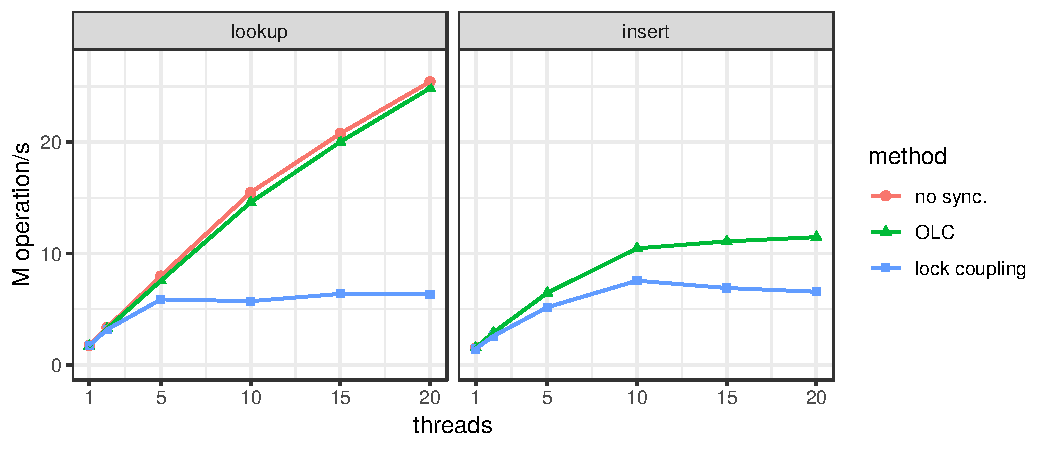
\includegraphics[width=\linewidth]{scale.pdf}
  \vspace{0.2cm}
  \caption{Scalability on 10-core system for B-tree operations (100M values).}
  \label{fig:scale}
\end{figure}

As Figure~\ref{fig:scale} shows, the results change dramatically once we use multiple threads.
For lookup, the scalability of OLC is near-linear up to 20 threads, even though the system has only 10 ``real cores''.
The OLC scalability for insert is also respectable (though not quite as linear because multi-threaded insertion approaches the memory bandwidth of our processor).
The figure also shows that the results of traditional lock coupling with read/write locks are significantly worse than OLC.
With 20 threads, lookup with OLC is 3.9$\times$ faster than traditional lock coupling.

\section{Summary}\label{sec:conc}

Optimistic Lock Coupling (OLC) is an effective synchronization method that combines the simplicity of traditional lock coupling with the superior scalability of lock-free approaches.
OLC is widely applicable and has already been successfully used to synchronize several data structures, including B-trees, binary search trees, and different trie variants.
These features make it highly attractive for modern database systems as well as performance-critical systems software in general.

\begin{thebibliography}{10}

\bibitem{DBLP:conf/spaa/BalmauGHZ16}
O.~Balmau, R.~Guerraoui, M.~Herlihy, and I.~Zablotchi.
\newblock Fast and robust memory reclamation for concurrent data structures.
\newblock In {\em SPAA}, 2016.

\bibitem{DBLP:journals/acta/BayerS77}
R.~Bayer and M.~Schkolnick.
\newblock Concurrency of operations on {B}-trees.
\newblock {\em Acta Informatica}, 9, 1977.

\bibitem{hot}
R.~Binna, E.~Zangerle, M.~Pichl, G.~Specht, and V.~Leis.
\newblock {HOT}: A height optimized trie index for main-memory database
  systems.
\newblock In {\em SIGMOD}, 2018.

\bibitem{DBLP:conf/ppopp/BronsonCCO10}
N.~G. Bronson, J.~Casper, H.~Chafi, and K.~Olukotun.
\newblock A practical concurrent binary search tree.
\newblock In {\em PPOPP}, 2010.

\bibitem{DBLP:conf/vldb/ChaHKK01}
S.~K. Cha, S.~Hwang, K.~Kim, and K.~Kwon.
\newblock Cache-conscious concurrency control of main-memory indexes on
  shared-memory multiprocessor systems.
\newblock In {\em VLDB}, 2001.

\bibitem{intel}
I.~Cutress.
\newblock {Intel} goes for 48-cores: {Cascade-AP} with multi-chip package
  coming soon.
\newblock
  \url{https://www.anandtech.com/show/13535/intel-goes-for-48cores-cascade-ap},
  2018 (accessed January, 2019).

\bibitem{DBLP:conf/cidr/FaleiroA17}
J.~M. Faleiro and D.~J. Abadi.
\newblock Latch-free synchronization in database systems: Silver bullet or
  fool's gold?
\newblock In {\em CIDR}, 2017.

\bibitem{DBLP:journals/ftdb/Graefe11}
G.~Graefe.
\newblock Modern {B}-tree techniques.
\newblock {\em Foundations and Trends in Databases}, 3(4), 2011.

\bibitem{DBLP:conf/hpca/KarnagelDRLLSL14}
T.~Karnagel, R.~Dementiev, R.~Rajwar, K.~Lai, T.~Legler, B.~Schlegel, and
  W.~Lehner.
\newblock Improving in-memory database index performance with
  {Intel}\({}^{\mbox{{\textregistered}}}\) transactional synchronization
  extensions.
\newblock In {\em HPCA}, 2014.

\bibitem{DBLP:journals/tods/LehmanY81}
P.~L. Lehman and S.~B. Yao.
\newblock Efficient locking for concurrent operations on {B}-trees.
\newblock {\em {ACM} Trans. Database Syst.}, 6(4), 1981.

\bibitem{leanstore}
V.~Leis, M.~Haubenschild, A.~Kemper, and T.~Neumann.
\newblock Leanstore: In-memory data management beyond main memory.
\newblock In {\em ICDE}, 2018.

\bibitem{art}
V.~Leis, A.~Kemper, and T.~Neumann.
\newblock The adaptive radix tree: {ARTful} indexing for main-memory databases.
\newblock In {\em ICDE}, 2013.

\bibitem{htmtkde}
V.~Leis, A.~Kemper, and T.~Neumann.
\newblock Scaling {HTM}-supported database transactions to many cores.
\newblock {\em {IEEE} Trans. Knowl. Data Eng.}, 28(2), 2016.

\bibitem{artsync}
V.~Leis, F.~Scheibner, A.~Kemper, and T.~Neumann.
\newblock The {ART} of practical synchronization.
\newblock In {\em DaMoN}, 2016.

\bibitem{DBLP:conf/icde/LevandoskiLS13a}
J.~J. Levandoski, D.~B. Lomet, and S.~Sengupta.
\newblock The {Bw}-tree: A {B}-tree for new hardware platforms.
\newblock In {\em ICDE}, 2013.

\bibitem{DBLP:journals/pvldb/MakreshanskiLS15}
D.~Makreshanski, J.~J. Levandoski, and R.~Stutsman.
\newblock To lock, swap, or elide: On the interplay of hardware transactional
  memory and lock-free indexing.
\newblock {\em {PVLDB}}, 8(11), 2015.

\bibitem{DBLP:dblp_conf/eurosys/MaoKM12}
Y.~Mao, E.~Kohler, and R.~T. Morris.
\newblock Cache craftiness for fast multicore key-value storage.
\newblock In {\em EuroSys}, 2012.

\bibitem{DBLP:journals/tpds/Michael04}
M.~M. Michael.
\newblock Hazard pointers: Safe memory reclamation for lock-free objects.
\newblock {\em {IEEE} Trans. Parallel Distrib. Syst.}, 15(6), 2004.

\bibitem{DBLP:journals/jacm/ShalevS06}
O.~Shalev and N.~Shavit.
\newblock Split-ordered lists: Lock-free extensible hash tables.
\newblock {\em J. {ACM}}, 53(3), 2006.

\bibitem{amd}
A.~Shilov.
\newblock {AMD} previews {EPYC} ‘{Rome}’ processor: Up to 64 {Zen} 2 cores.
\newblock
  \url{https://www.anandtech.com/show/13561/amd-previews-epyc-rome-processor-up-to-64-zen-2-cores},
  2018 (accessed January, 2019).

\bibitem{DBLP:conf/sosp/TuZKLM13}
S.~Tu, W.~Zheng, E.~Kohler, B.~Liskov, and S.~Madden.
\newblock Speedy transactions in multicore in-memory databases.
\newblock In {\em SOSP}, 2013.

\bibitem{buzzword}
Z.~Wang, A.~Pavlo, H.~Lim, V.~Leis, H.~Zhang, M.~Kaminsky, and D.~Andersen.
\newblock Building a {Bw}-tree takes more than just buzz words.
\newblock In {\em SIGMOD}, 2018.

\end{thebibliography}


%\bibliographystyle{abbrv}
%\bibliography{main}

\end{document}

\end{article}



\begin{article}
{Ethical Challenges in the Future of Work}
{Pierre Bourhis, Gianluca Demartini, Shady Elbassuoni, Emile Hoareau, H. Raghav Rao}
\graphicspath{{submissions/automl/}}
\pdfminorversion=5
\documentclass[11pt]{article}
\usepackage{deauthor,times,graphicx,caption,microtype}
\usepackage{hyperref}
\usepackage{listings}
\usepackage{booktabs}

\begin{document}

\title{Optimistic Lock Coupling: A Scalable and Efficient General-Purpose Synchronization Method}

\author{Viktor Leis, Michael Haubenschild\raisebox{0.9ex}{$\ast$}, Thomas Neumann\\ Technische Universit{\"a}t M{\"u}nchen \hspace{0.7cm} Tableau Software\raisebox{0.9ex}{$\ast$} \\ {\{leis,neumann\}{@}in.tum.de} \hspace{0.7cm} {mhaubenschild{@}tableau.com\raisebox{0.9ex}{$\ast$}}}

\maketitle

\begin{abstract}
As the number of cores on commodity processors continues to increase, scalability becomes more and more crucial for overall performance.
Scalable and efficient concurrent data structures are particularly important, as these are often the building blocks of parallel algorithms.
Unfortunately, traditional synchronization techniques based on fine-grained locking have been shown to be unscalable on modern multi-core CPUs.
Lock-free data structures, on the other hand, are extremely difficult to design and often incur significant overhead.

In this work, we make the case for Optimistic Lock Coupling as a practical alternative to both traditional locking and the lock-free approach.
We show that Optimistic Lock Coupling is highly scalable and almost as simple to implement as traditional lock coupling.
Another important advantage is that it is easily applicable to most tree-like data structures.
We therefore argue that Optimistic Lock Coupling, rather than a complex and error-prone custom synchronization protocol, should be the default choice for performance-critical data structures.
\end{abstract}

\section{Introduction}

% more and more cores
Today, Intel's commodity server processors have up to 28 cores and its upcoming microarchitecture will have up to 48 cores per socket~\cite{intel}.
Similarly, AMD currently stands at 32 cores and this number is expected to double in the next generation~\cite{amd}.
Since both platforms support simultaneous multithreading (also known as hyperthreading), affordable commodity servers (with up to two sockets) will soon routinely have between 100 and 200 hardware threads.

% data structure scalability is important
With such a high degree of hardware parallelism, efficient data processing crucially depends on how well concurrent data structures scale.
Internally, database systems use a plethora of data structures like table heaps, internal work queues, and, most importantly, index structures.
Any of these can easily become a scalability (and therefore overall performance) bottleneck on many-core CPUs.

% traditional synchronization: fine-grained locks, slow, cache invalidation
Traditionally, database systems synchronize internal data structures using fine-grained reader/writer locks\footnote{In this work, we focus on data structure synchronization rather than high-level transaction semantics and therefore use the term {\em lock} for what would typically be called {\em latch} in the database literature. We thus follow common computer science (rather than database) terminology.}.
Unfortunately, while fine-grained locking makes lock contention unlikely, it still results in bad scalability because lock acquisition and release require writing to shared memory.
Due to the way cache coherency is implemented on modern multi-core CPUs, these writes cause additional cache misses\footnote{The cache coherency protocol ensures that all copies of a cache line on other cores are invalidated before the write can proceed.} and the cache line containing the lock's internal data becomes a point of physical contention.
As a result, any frequently-accessed lock (e.g., the lock of the root node of a B-tree) severely limits scalability.

% lock-free bw-tree: no more latches, but indirections, extremely complex
Lock-free data structures like the Bw-tree~\cite{DBLP:conf/icde/LevandoskiLS13a} (a lock-free B-tree variant) or the Split-Ordered List~\cite{DBLP:journals/jacm/ShalevS06} (a lock-free hash table) do not acquire any locks and therefore generally scale much better than locking-based approaches (in particular for read-mostly workloads).
However, lock-free synchronization has other downsides:
First, it is very difficult and results in extremely complex and error-prone code (when compared to locking).
Second, because the functionality of atomic primitives provided by the hardware (e.g., atomically compare-and-swap 8 bytes) is limited, complex operations require additional indirections within the data structure.
For example, the Bw-tree requires an indirection table and the Split-Ordered List requires ``dummy nodes'', resulting in overhead due to additional cache misses.

% OLC for the win
In this paper we make the case for {\em Optimistic Lock Coupling (OLC)}, a synchronization method that combines some of the best properties of lock-based and lock-free synchronization.
OLC utilizes a special lock type that can be used in two modes:
The first mode is similar to a traditional mutex and excludes other threads by physically acquiring the underlying lock.
In the second mode, reads can proceed optimistically by validating a version counter that is embedded in the lock (similar to optimistic concurrency control).
The first mode is typically used by writers and the second mode by readers.
Besides this special lock type, OLC is based on the observation that optimistic lock validations can be interleaved/coupled---similar to the pair-wise interleaved lock acquisition of traditional lock coupling.
Hence, the name Optimistic Lock Coupling.

OLC has a number of desirable features:
\begin{itemize}
\item By reducing the number of writes to shared memory locations and thereby avoiding cache invalidations, it {\bf scales well} for most workloads.
\item In comparison to unsynchronized code, it requires few additional CPU instructions making it {\bf efficient}.
\item OLC is {\bf widely applicable} to different data structures. It has already been successfully used for synchronizing binary search trees~\cite{DBLP:conf/ppopp/BronsonCCO10}, tries~\cite{artsync}, trie/B-tree hybrids~\cite{DBLP:dblp_conf/eurosys/MaoKM12}, and B-trees~\cite{buzzword}.
\item In comparison to the lock-free paradigm, it is also {\bf easy to use} and requires few modifications to existing, single-threaded data structures.
\end{itemize}
Despite these positive features and its simplicity, OLC is not yet widely known.
The goal of this paper is therefore to popularize this simple idea and to make a case for it.
We argue that OLC deserves to be widely known.
It is a good default synchronization paradigm---more complex, data structure-specific protocols are seldom beneficial.

The rest of the paper is organized as follows.
Section~\ref{sec:related} discusses related work, tracing the history of OLC and its underlying ideas in the literature.
The core of the paper is Section~\ref{sec:olc}, which describes the ideas behind OLC and how it can be used to synchronize complex data structures.
In Section~\ref{sec:evaluation} we experimentally show that OLC has low overhead and scales well when used to synchronize an in-memory B-tree.
We summarize the paper in Section~\ref{sec:conc}.

\newpage
\section{Related Work}\label{sec:related}

Lock coupling has been proposed as a method for allowing concurrent operations on B-trees in 1977~\cite{DBLP:journals/acta/BayerS77}.
This traditional and still widely-used method, described in detail in Graefe's B-tree survey~\cite{DBLP:journals/ftdb/Graefe11}, is also called ``latch coupling'', ``hand-over-hand locking'', and ``crabbing''.
Because at most two locks are held at-a-time during tree traversal, this technique seemingly allows for a high degree of parallelism---in particular if read/write locks are used to enable inner nodes to be locked in shared mode.
However, as we show in Section~\ref{sec:evaluation}, on modern hardware lock acquisition (even in shared mode) results in suboptimal scalability.

An early alternative from 1981 is a B-tree variant called B-link tree~\cite{DBLP:journals/tods/LehmanY81}, which only holds a single lock at a time.
It is based on the observation that between the release of the parent lock and the acquisition of the child lock, the only ``dangerous'' thing that could have happened is the split of a child node (assuming one does not implement merge operations).
Thus, when a split happens, the key being searched might end up on a neighboring node to the right of the current child node.
A B-link tree traversal therefore detects this condition and, if needed, transparently proceeds to the neighboring node.
Releasing the parent lock early is highly beneficial when the child node needs to be fetched from disk.
For in-memory workloads, however, the B-link tree has the same scalability issues as lock coupling (it acquires just as many locks).

The next major advance, Optimistic Latch-Free Index Traversal (OLFIT)~\cite{DBLP:conf/vldb/ChaHKK01}, was proposed in 2001.
OLFIT introduced the idea of a combined lock/update counter, which we call {\em optimistic lock}. % , for lack of a better name,
Based on these per-node optimistic locks and the synchronization protocol of the B-link tree, OLFIT finally achieves good scalability on parallel processors.
The OLFIT protocol is fairly complex, as it requires both the non-trivial B-link protocol and optimistic locks.
Furthermore, like the B-link tree protocol, it does not support merging nodes, and is specific to B-trees (cannot easily be applied to other data structures).

In the following two decades, the growth of main-memory capacity led to much research into other data structures besides the venerable B-tree.
Particularly relevant for our discussion is Bronson et al.'s~\cite{DBLP:conf/ppopp/BronsonCCO10} concurrent binary search tree, which is based on optimistic version validation and has a sophisticated, data structure-specific synchronization protocol.
To the best of our knowledge, this 2010 paper is the first that, as part of its protocol, interleaves version validation across nodes---rather than validating each node separately like OLFIT.
In that paper, this idea is called ``hand-over-hand, optimistic validation'', while we prefer the term Optimistic Lock Coupling to highlight the close resemblance to traditional lock coupling.
Similarly, Mao et al.'s~\cite{DBLP:dblp_conf/eurosys/MaoKM12} Masstree (a concurrent hybrid trie/B-tree) is also based on the same ideas, but again uses them as part of a more complex protocol.

The Adaptive Radix Tree (ART)~\cite{art} is another recent in-memory data structure, which we proposed in 2013.
In contrast to the two data structures just mentioned, it was originally designed with single-threaded performance in mind without supporting concurrency.
To add support for concurrency, we initially started designing a custom protocol called Read-Optimized Write Exclusion (ROWEX)~\cite{artsync}, which turned out to be non-trivial and requires modifications of the underlying data structure\footnote{Note that ROWEX is already easier to apply to existing data structures than the lock-free approach. The difficulty depends on the data structure. Applying ROWEX is hard for B-trees with sorted keys and fairly easy for copy-on-write data structures like the Height Optimized Trie~\cite{hot}---with ART being somewhere in the middle.}.
However, fairly late in the project, we also realized, that OLC {\em alone} (rather than as part of a more complex protocol) is sufficient to synchronize ART.
No other changes to the data structure were necessary.
Both approaches were published and experimentally evaluated in a followup paper~\cite{artsync}, which shows that, despite its simplicity, OLC is efficient, scalable, and generally outperforms ROWEX.

Similar results were recently published regarding B-trees~\cite{buzzword}.
In this experimental study a simple OLC-based synchronization outperformed the Bw-tree~\cite{DBLP:conf/icde/LevandoskiLS13a}, a complex lock-free synchronization approach.
Another recent paper shows that for write-intensive workloads, locking often performs better than lock-free synchronization~\cite{DBLP:conf/cidr/FaleiroA17}.
These experiences indicate that OLC is a general-purpose synchronization paradigm and motivate the current paper.

%foster b-tree\cite{DBLP:journals/tods/GraefeKK12}
%Shasha theory~\cite{DBLP:journals/tods/ShashaG88}

\section{Optimistic Lock Coupling}\label{sec:olc}

% locks suck
The standard technique for inter-thread synchronization is mutual exclusion using fine-grained locks.
In a B-tree, for example, every node usually has its own associated lock, which is acquired before accessing that node.
The problem of locking on modern multi- and many-core processors is that lock acquisition and release require writing to the shared memory location that implements the lock.
This write causes exclusive ownership of the underlying cache line and invalidates copies of it on all other processor cores.
For hierarchical, tree-like data structures, the lock of the root node becomes a point of physical contention---even in read-only workloads and even when read/write locks are used.
Depending on the specific data structure, number of cores, cache coherency protocol implementation, cache topology, whether Non-Uniform Memory Access (NUMA) is used, locking can even result in multi-threaded performance that is worse than single-threaded execution.

% in b-trees this happens very much
The inherent pessimism of locking is particularly unfortunate for B-trees:
Despite the fact that logical modifications of the root node are very infrequent, every B-tree operation must lock the root node during tree traversal\footnote{To a lesser extent this obviously applies to all inner nodes, not just the root.}.
Even the vast majority of update operations (with the exception of splits and merges), only modify a single leaf node.
These observations indicate that a more optimistic approach, which does not require locking inner nodes, would be very beneficial for B-trees.

\subsection{Optimistic Locks}

% optimism to the rescue
As the name indicates, optimistic locks try to solve the scalability issues of traditional locks using an optimistic approach.
Instead of always physically acquiring locks, even for nodes that are unlikely to be modified simultaneously, after-the-fact validation is used to detect conflicts.
This is done by augmenting each lock with a version/update counter that is incremented on every modification.
Using this version counter, readers can optimistically proceed before validating that the version did not change to ensure that the read was safe.
If validation fails, the operation is restarted.

% details on opt locks
Using optimistic locks, a read-only node access (i.e., the majority of all operations in a B-tree) does not acquire the lock and does not increment the version counter.
Instead, it performs the following steps:
\begin{enumerate}
\item read lock version (restart if lock is not free)
\item access node
\item read the version again and validate that it has not changed in the meantime
\end{enumerate}
If the last step (the validation) fails, the operation has to be restarted.
Write operations, on the other hand, are more similar to traditional locking:
\begin{enumerate}
\item acquire lock (wait if necessary)
\item access/write to node
\item increment version and unlock node
\end{enumerate}
Writes can therefore protect a node from other writes.

% similar to locks
As we observed in an earlier paper~\cite{artsync}, because of similar semantics, optimistic locks can be hidden behind an API very similar to traditional read/write locks.
Both approaches have an exclusive lock mode, and acquiring a traditional lock in shared mode is analogous to optimistic version validation.
Furthermore, like with some implementations of traditional read/write locks, optimistic locks allow upgrading a shared lock to an exclusive lock.
Lock upgrades are, for example, used to avoid most B-tree update operations from having to lock inner nodes.
In our experience, the close resemblance of optimistic and traditional locks simplifies the reasoning about optimistic locks;
one can apply similar thinking as in traditional lock-based protocols.

\subsection{Lock Coupling with Optimistic Locks}

\begin{figure}
  \centering
  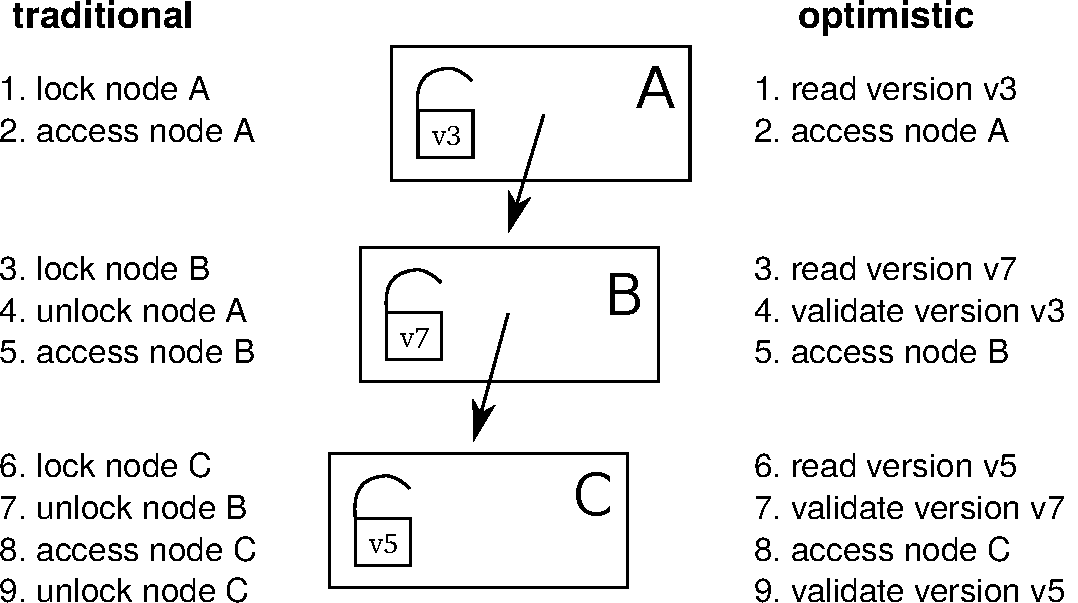
\includegraphics[width=0.65\linewidth]{olcall.pdf}
  \vspace{0.2cm}
  \caption{Comparison of a lookup operation in a 3-level tree using traditional lock coupling (left-hand side) vs.~optimistic lock coupling (right-hand side).}
  \label{fig:olc}
\end{figure}

The traditional and most common lock-based synchronization protocol for B-trees is lock coupling, which interleaves lock acquisitions while holding at most two locks at a time.
If, as we observed earlier, optimistic locks have similar semantics as traditional locks, it is natural to ask whether lock coupling can be combined with optimistic locks.
And indeed the answer is yes: One can almost mechanically translate traditional lock coupling code to optimistic lock coupling code.
This is illustrated in Figure~\ref{fig:olc}, which compares the traversal in a tree of height 3 using traditional and optimistic locks.
As the figure shows, the main difference is that locking is translated to reading the version and that unlocking becomes validation of the previously read version.
This simple change provides efficient lock-free tree traversal without the need to design a complex synchronization protocol.

It is important to emphasize the conceptual simplicity of OLC in comparison to data structures that use custom protocols like the Bw-tree~\cite{DBLP:conf/icde/LevandoskiLS13a}.
To implement lock-free access, the Bw-tree requires an indirection table, delta nodes, complex splitting and merging logic, retry logic, etc.
OLC, on the other hand, can directly be applied to B-trees mostly by adding the appropriate optimistic locking code and without modifying the node layout itself.
Therefore, OpenBw-Tree, an open source implementation of the Bw-tree, requires an order of magnitude more code than a B-tree based on OLC\footnote{Both implementations are available on GitHub: \url{https://github.com/wangziqi2016/index-microbench}}.
Given how difficult it is to develop, validate, and debug lock-free code, simplicity is obviously a major advantage.

\subsection{Correctness Aspects}

\begin{figure}
  % \centering
  %[basicstyle=\normalsize\ttfamily,showstringspaces=false,columns=fullflexible,breaklines=false,breakatwhitespace=true,numbers=none,numberstyle=\small,style=C,keepspaces=true]
\begin{lstlisting}[basicstyle=\ttfamily,language=C++,numbers=left,numberstyle=\small]
std::atomic<BTreeNode*> root;

// search for key in B+tree, returns payload in resultOut
bool lookup(Key key, Value& resultOut) {
   BTreeNode* node = root.load();
   uint64_t nodeVersion = node->readLockOrRestart();
   if (node != root.load()) // make sure the root is still the root
      restart();

   BTreeInner<Key>* parent = nullptr;
   uint64_t parentVersion = 0;

   while (node->isInner()) {
      auto inner = (BTreeInner*)node;

      // unlock parent and make current node the parent
      if (parent)
         parent->readUnlockOrRestart(parentVersion);
      parent = inner;
      parentVersion = nodeVersion;

      // search for next node
      node = inner->findChild(key);
      // validate 'inner' to ensure that 'node' pointer is valid
      inner->checkOrRestart(nodeVersion);
      // now it safe to dereference 'node' pointer (read its version)
      nodeVersion = node->readLockOrRestart();
   }

   // search in leaf and retrieve payload
   auto leaf = (BTreeLeaf*)node;
   bool success = leaf->findValue(key, resultOut);

   // unlock everything
   if (parent)
      parent->readUnlockOrRestart(parentVersion);
   node->readUnlockOrRestart(nodeVersion);

   return success;
}
\end{lstlisting}
  \vspace{0.2cm}
  \caption{B-tree lookup code using OLC. For simplicity, the restart logic is not shown.}
  \label{fig:lookup}
\end{figure}

So far, we have introduced the high-level ideas behind OLC and have stressed its similarity to traditional lock coupling.
Let us now discuss some cases where the close similarity between lock coupling and OLC breaks down.
To make this more concrete, we show the B-tree lookup code in Figure~\ref{fig:lookup}.
In the code, \texttt{readLockOrRestart} reads the lock version and \texttt{readUnlockOrRestart} validates that the read was correct.

One issue with OLC is that any pointer speculatively read from a node may point to invalid memory (if that node is modified concurrently).
Dereferencing such a pointer (e.g., to read its optimistic lock), may cause a segmentation fault or undefined behavior.
In the code shown in Figure~\ref{fig:lookup}, this problem is prevented by the extra check in line 25, which ensures that the read from the node containing the pointer was correct.
Without this additional validation, the code would in line 27 dereference the pointer speculatively read in line 23.
Note that the implementation of \texttt{checkOrRestart} is actually identical to \texttt{readUnlockOrRestart}.
We chose to give it a different name to highlight the fact that this extra check would not be necessary with read/write locks.

Another potential issue with optimistic locks is code that does not terminate.
Code that speculatively accesses a node, like an intra-node binary search, should be written in a way such that it always terminates---even in the presence of concurrent writes.
Otherwise, the validation code that detects the concurrent write will never run.
The binary search of a B-tree, for example, needs to be written in such a way that each comparison makes progress.
For some data structures that do not require loops in the traversal code (like ART) termination is trivially true.

\subsection{Implementation Details}

% implementation, efficiency
To implement an optimistic lock, one can combine the lock and the version counter into a single 64-bit\footnote{Even after subtracting one bit for the lock status, a back-of-the-envelope calculation can show that 63 bits are large enough to never overflow in practice.} word~\cite{artsync}.
A typical read operation will therefore merely consist of reading this version counter atomically.
In C++11 this can be implemented using the \texttt{std::atomic} type.

On x86, atomic reads are cheap because of x86's strong memory order guarantees.
No memory fences are required for sequentially-consistent loads, which are translated (by both GCC and clang) into standard \texttt{MOV} instructions.
Hence, the only effect of \texttt{std::atomic} for loads is preventing instruction re-ordering.
This makes version access and validation cheap.
Acquiring and releasing an optimistic lock in exclusive mode has comparable cost to a traditional lock:
A fairly expensive sequentially-consistent store is needed for acquiring a lock, while a standard \texttt{MOV} suffices for releasing it.
A simple sinlock-based implementation of optimistic locks can be found in the appendix of an earlier paper~\cite{artsync}.

OLC code must be able to handle restarts since validation or lock upgrade can fail due to concurrent writers.
Restarts can easily be implemented by wrapping the data structure operation in a loop (for simplicity not shown in Figure~\ref{fig:lookup}).
Such a loop also enables limiting the number of optimistic retry operations and falling back to pessimistic locking in cases of very heavy contention.
The ability to fall back to traditional locking is a major advantage of OLC in terms of robustness over lock-free approaches, which do not have this option.

In addition to the optimistic shared mode and the exclusive mode, optimistic locks also support a ``shared pessimistic'' mode, which physically acquires the lock in shared mode (allowing multiple concurrent readers but no writers).
This mode is useful for table (or range) scans that touch many tuples on a leaf page (which would otherwise easily abort).
Finally, let us mention that large range scans and table scans, should be broken up into several per-node traversals as is done in the LeanStore~\cite{leanstore} system.

Like all lock-free data structures, but unlike traditional locking and Hardware Transactional Memory~\cite{DBLP:conf/hpca/KarnagelDRLLSL14,DBLP:journals/pvldb/MakreshanskiLS15,htmtkde}, OLC requires care when deleting (and reusing) nodes.
The reason is that a deleting thread can never be sure that a node can be reclaimed because other threads might still be optimistically reading from that node.
Therefore, standard solutions like epoch-based reclamation~\cite{DBLP:conf/sosp/TuZKLM13}, hazard pointers~\cite{DBLP:journals/tpds/Michael04}, or optimized hazard pointers~\cite{DBLP:conf/spaa/BalmauGHZ16} need to be used.
These memory reclamation techniques are, however, largely orthogonal to the synchronization protocol itself.

%-lock-free is not a strong guarantee

\newpage
\section{Evaluation}\label{sec:evaluation}

Let us now experimentally evaluate the overhead and scalability of OLC.
For the experiments, we use an in-memory B+tree implemented in C++11 using templates, which is configured to use nodes of 4096 bytes, random 8 byte keys, and 8 byte payloads.
Based on this B-tree, we compare the following synchronization approaches:
\begin{itemize}
\item an OLC implementation\footnote{An almost identical OLC implementation is available on github: \url{https://github.com/wangziqi2016/index-microbench/tree/master/BTreeOLC}}
\item a variant based on traditional lock coupling and read/write locks
\item the unsynchronized B-tree, which obviously is only correct for read-only workloads but allows measuring the overhead of synchronization
\end{itemize}
Note that earlier work has compared the OLC implementation with a Bw-tree implementation~\cite{buzzword} and other state-of-the-art in-memory index structures.

We use a Haswell EP system with an Intel Xeon E5-2687W v3 CPU, which has 10 cores (20 ``Hyper-Threads'') and 25~MB of L3 cache.
The system is running Ubuntu 18.10 and we use GCC 8.2.0 to compile our code.
The CPU counters are obtained using the Linux perf API\footnote{We use the following convenience wrapper: \url{https://github.com/viktorleis/perfevent}}.

\begin{table}
  \caption{Performance and CPU counters for lookup and insert operations in a B-tree with 100M keys. We perform 100M operations and normalize the CPU counters by that number.}
  \label{tab:overhead}
  \centering
  \begin{tabular}{lrrrrrrr}\toprule
                    &         &        &        & instruc-  & L1     & L3     & branch \\
                    & threads & M op/s & cycles & tions & misses & misses & misses \\\midrule
lookup (no sync.)   & 1       & 1.72   & 2028   & 283     & 39.1   & 14.9   & 16.1   \\
lookup (OLC)        & 1       & 1.65   & 2107   & 370     & 43.9   & 15.1   & 16.7   \\
lookup (lock coup.) & 1       & 1.72   & 2078   & 365     & 42.3   & 16.9   & 15.7   \\\midrule
insert (no sync.)   & 1       & 1.51   & 2286   & 530     & 59.8   & 31.1   & 17.3   \\
insert (OLC)        & 1       & 1.50   & 2303   & 629     & 61.2   & 31.1   & 16.5   \\
insert (lock coup.) & 1       & 1.41   & 2473   & 644     & 61.0   & 31.0   & 17.2   \\\midrule
lookup (no sync.)   & 10      & 15.48  & 2058   & 283     & 38.6   & 15.5   & 16.0   \\
lookup (OLC)        & 10      & 14.60  & 2187   & 370     & 43.8   & 15.8   & 16.8   \\
lookup (lock coup.) & 10      & 5.71   & 5591   & 379     & 54.2   & 17.0   & 14.8   \\\midrule
insert (no sync.)   & 10      & -      & -      & -       & -      & -      & -      \\
insert (OLC)        & 10      & 10.46  & 2940   & 656     & 62.0   & 32.5   & 16.8   \\
insert (lock coup.) & 10      & 7.55   & 4161   & 667     & 75.0   & 28.6   & 16.2   \\
    \bottomrule
\end{tabular}
\end{table}

Table~\ref{tab:overhead} compares the performance and CPU counters for lookup and insert operations in a B-tree with 100M keys.
With {\em single-threaded} execution, we observe that all three approaches have very similar performance.
Adding traditional or optimistic locks to unsynchronized B-tree code results in up to 30\% of additional instructions without affecting single-threaded performance much.

\begin{figure}
  \centering
  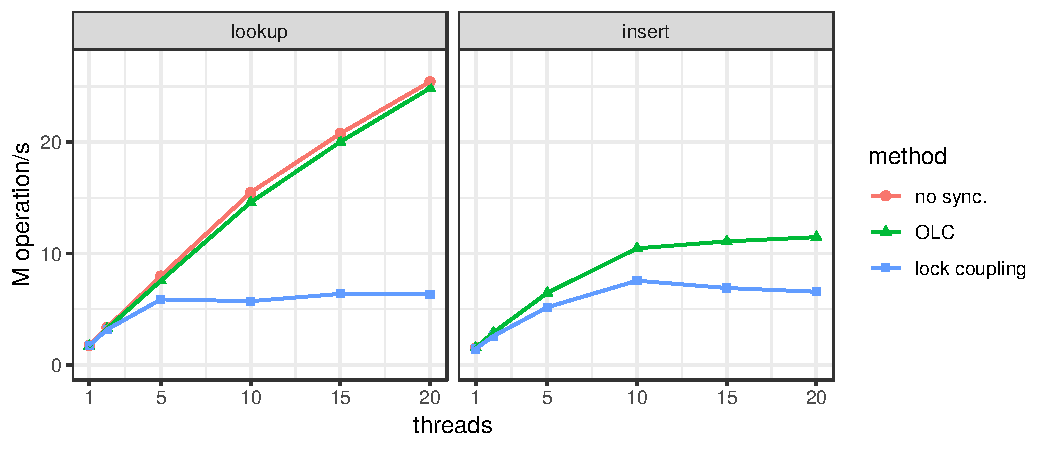
\includegraphics[width=\linewidth]{scale.pdf}
  \vspace{0.2cm}
  \caption{Scalability on 10-core system for B-tree operations (100M values).}
  \label{fig:scale}
\end{figure}

As Figure~\ref{fig:scale} shows, the results change dramatically once we use multiple threads.
For lookup, the scalability of OLC is near-linear up to 20 threads, even though the system has only 10 ``real cores''.
The OLC scalability for insert is also respectable (though not quite as linear because multi-threaded insertion approaches the memory bandwidth of our processor).
The figure also shows that the results of traditional lock coupling with read/write locks are significantly worse than OLC.
With 20 threads, lookup with OLC is 3.9$\times$ faster than traditional lock coupling.

\section{Summary}\label{sec:conc}

Optimistic Lock Coupling (OLC) is an effective synchronization method that combines the simplicity of traditional lock coupling with the superior scalability of lock-free approaches.
OLC is widely applicable and has already been successfully used to synchronize several data structures, including B-trees, binary search trees, and different trie variants.
These features make it highly attractive for modern database systems as well as performance-critical systems software in general.

\begin{thebibliography}{10}

\bibitem{DBLP:conf/spaa/BalmauGHZ16}
O.~Balmau, R.~Guerraoui, M.~Herlihy, and I.~Zablotchi.
\newblock Fast and robust memory reclamation for concurrent data structures.
\newblock In {\em SPAA}, 2016.

\bibitem{DBLP:journals/acta/BayerS77}
R.~Bayer and M.~Schkolnick.
\newblock Concurrency of operations on {B}-trees.
\newblock {\em Acta Informatica}, 9, 1977.

\bibitem{hot}
R.~Binna, E.~Zangerle, M.~Pichl, G.~Specht, and V.~Leis.
\newblock {HOT}: A height optimized trie index for main-memory database
  systems.
\newblock In {\em SIGMOD}, 2018.

\bibitem{DBLP:conf/ppopp/BronsonCCO10}
N.~G. Bronson, J.~Casper, H.~Chafi, and K.~Olukotun.
\newblock A practical concurrent binary search tree.
\newblock In {\em PPOPP}, 2010.

\bibitem{DBLP:conf/vldb/ChaHKK01}
S.~K. Cha, S.~Hwang, K.~Kim, and K.~Kwon.
\newblock Cache-conscious concurrency control of main-memory indexes on
  shared-memory multiprocessor systems.
\newblock In {\em VLDB}, 2001.

\bibitem{intel}
I.~Cutress.
\newblock {Intel} goes for 48-cores: {Cascade-AP} with multi-chip package
  coming soon.
\newblock
  \url{https://www.anandtech.com/show/13535/intel-goes-for-48cores-cascade-ap},
  2018 (accessed January, 2019).

\bibitem{DBLP:conf/cidr/FaleiroA17}
J.~M. Faleiro and D.~J. Abadi.
\newblock Latch-free synchronization in database systems: Silver bullet or
  fool's gold?
\newblock In {\em CIDR}, 2017.

\bibitem{DBLP:journals/ftdb/Graefe11}
G.~Graefe.
\newblock Modern {B}-tree techniques.
\newblock {\em Foundations and Trends in Databases}, 3(4), 2011.

\bibitem{DBLP:conf/hpca/KarnagelDRLLSL14}
T.~Karnagel, R.~Dementiev, R.~Rajwar, K.~Lai, T.~Legler, B.~Schlegel, and
  W.~Lehner.
\newblock Improving in-memory database index performance with
  {Intel}\({}^{\mbox{{\textregistered}}}\) transactional synchronization
  extensions.
\newblock In {\em HPCA}, 2014.

\bibitem{DBLP:journals/tods/LehmanY81}
P.~L. Lehman and S.~B. Yao.
\newblock Efficient locking for concurrent operations on {B}-trees.
\newblock {\em {ACM} Trans. Database Syst.}, 6(4), 1981.

\bibitem{leanstore}
V.~Leis, M.~Haubenschild, A.~Kemper, and T.~Neumann.
\newblock Leanstore: In-memory data management beyond main memory.
\newblock In {\em ICDE}, 2018.

\bibitem{art}
V.~Leis, A.~Kemper, and T.~Neumann.
\newblock The adaptive radix tree: {ARTful} indexing for main-memory databases.
\newblock In {\em ICDE}, 2013.

\bibitem{htmtkde}
V.~Leis, A.~Kemper, and T.~Neumann.
\newblock Scaling {HTM}-supported database transactions to many cores.
\newblock {\em {IEEE} Trans. Knowl. Data Eng.}, 28(2), 2016.

\bibitem{artsync}
V.~Leis, F.~Scheibner, A.~Kemper, and T.~Neumann.
\newblock The {ART} of practical synchronization.
\newblock In {\em DaMoN}, 2016.

\bibitem{DBLP:conf/icde/LevandoskiLS13a}
J.~J. Levandoski, D.~B. Lomet, and S.~Sengupta.
\newblock The {Bw}-tree: A {B}-tree for new hardware platforms.
\newblock In {\em ICDE}, 2013.

\bibitem{DBLP:journals/pvldb/MakreshanskiLS15}
D.~Makreshanski, J.~J. Levandoski, and R.~Stutsman.
\newblock To lock, swap, or elide: On the interplay of hardware transactional
  memory and lock-free indexing.
\newblock {\em {PVLDB}}, 8(11), 2015.

\bibitem{DBLP:dblp_conf/eurosys/MaoKM12}
Y.~Mao, E.~Kohler, and R.~T. Morris.
\newblock Cache craftiness for fast multicore key-value storage.
\newblock In {\em EuroSys}, 2012.

\bibitem{DBLP:journals/tpds/Michael04}
M.~M. Michael.
\newblock Hazard pointers: Safe memory reclamation for lock-free objects.
\newblock {\em {IEEE} Trans. Parallel Distrib. Syst.}, 15(6), 2004.

\bibitem{DBLP:journals/jacm/ShalevS06}
O.~Shalev and N.~Shavit.
\newblock Split-ordered lists: Lock-free extensible hash tables.
\newblock {\em J. {ACM}}, 53(3), 2006.

\bibitem{amd}
A.~Shilov.
\newblock {AMD} previews {EPYC} ‘{Rome}’ processor: Up to 64 {Zen} 2 cores.
\newblock
  \url{https://www.anandtech.com/show/13561/amd-previews-epyc-rome-processor-up-to-64-zen-2-cores},
  2018 (accessed January, 2019).

\bibitem{DBLP:conf/sosp/TuZKLM13}
S.~Tu, W.~Zheng, E.~Kohler, B.~Liskov, and S.~Madden.
\newblock Speedy transactions in multicore in-memory databases.
\newblock In {\em SOSP}, 2013.

\bibitem{buzzword}
Z.~Wang, A.~Pavlo, H.~Lim, V.~Leis, H.~Zhang, M.~Kaminsky, and D.~Andersen.
\newblock Building a {Bw}-tree takes more than just buzz words.
\newblock In {\em SIGMOD}, 2018.

\end{thebibliography}


%\bibliographystyle{abbrv}
%\bibliography{main}

\end{document}

\end{article}



\end{articlesection}

% put the news items below- there can be multiple news sections
% each with its own title
% news will usually have an author as well as a title, 
% e.g. TCDE elections
% news articles are in the same format as letters
% typically, news articles will be stored in a directory called "news"

%\begin{newssection}{News headline}

% insert news items here; news will typically have authors
% see the Sept. 2018 issue for an example

%\begin{news}{news item title}
%{author name}{author affiliation}
%\input{news/news-article.tex}
%\end{news}
%
%\newpage


%\end{newssection}



\begin{callsection}

%  This section will be empty for your version
%
%  Calls for papers section.  Use the callsection environment.
%  Each call for papers is contained in an call environment, where the single 
%  required options to \begin{call} is the name of the conference.
% typically calls are stored in a "calls" directory
%
%\begin{call}{name of conference}
%\centerline{\includegraphics[width=\textwidth, bb= 0 0 590 760]{calls/conference-name.pdf}}
%\end{call}
%\begin{call}{ICDE 2019 Conference}
%\centerline{
\includegraphics[width=\textwidth, bb= 0 0 610 790] {../Dec-2018/calls/icde19.pdf}} 
%\centerline{
\includegraphics[width=\textwidth, bb= 0 0 590 760] {calls/icde19.pdf}}
%\end{call}
\begin{call}{TCDE Membership Form}
%\centerline{\includegraphics[width=\textwidth, bb= 0 0 610 790]
\centerline{
\includegraphics[width=\textwidth, bb= 0 0 590 760] {../Dec-2018/calls/tcde.pdf}}
\end{call}

\end{callsection}

\end{bulletin}
\end{document}
